\subsubsection{Calculate the axle weights}
\label{section:calculating_axle_weights}
The axle weights used to calculate the influence lines are as in table \ref{table:axle_weights}. These are as discussed in chapter method something!!. The system setup described in section \ref{system_setup}, gives us three different locaions for measuring strain and so we have three diffferent influence lines generated by the BWIM program. When calculating the axle weights corresponding to each train, we will then have three different estimates of the axle weights.

\begin{figure}[h]
	\begin{subfigure}[t]{0.3\textwidth}
		% This file was created by matlab2tikz.
%
%The latest updates can be retrieved from
%  http://www.mathworks.com/matlabcentral/fileexchange/22022-matlab2tikz-matlab2tikz
%where you can also make suggestions and rate matlab2tikz.
%
\definecolor{mycolor1}{rgb}{0.00000,0.44700,0.74100}%
%
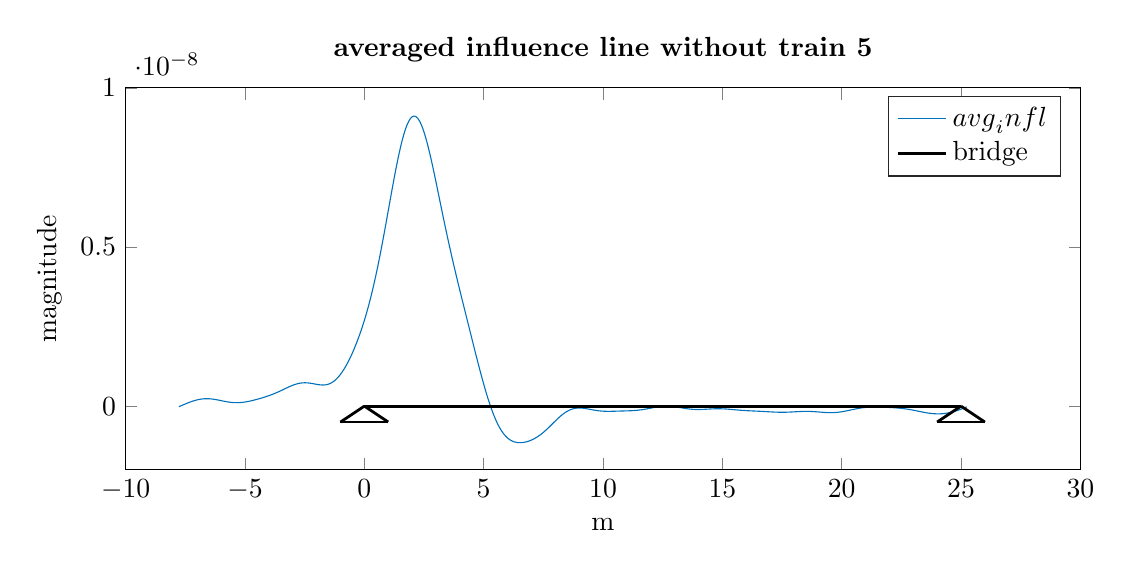
\begin{tikzpicture}
  
  \begin{axis}[%
    width=\textwidth,
    height=0.4\textwidth,
    at={(0\textwidth,0\textwidth)},
    scale only axis,
    xmin=-10,
    xmax=30,
    xlabel={m},
    ymin=-2e-09,
    ymax=1e-08,
    ylabel={magnitude},
    axis background/.style={fill=white},
    title style={font=\bfseries},
    title={averaged influence line without train 5},
    legend style={legend cell align=left,align=left,draw=white!15!black}
    ]
    \addplot [color=mycolor1,solid]
    table[row sep=crcr]{%
    -7.7680634765625	-1.76699119538898e-11\\
    -7.7479140625	-1.1284383338611e-11\\
    -7.7277646484375	-4.87819900584435e-12\\
    -7.707615234375	1.54404850015636e-12\\
    -7.6874658203125	7.97767654315349e-12\\
    -7.66731640625	1.44179146751862e-11\\
    -7.6471669921875	2.08599073029194e-11\\
    -7.627017578125	2.72987167527774e-11\\
    -7.6068681640625	3.37293267459539e-11\\
    -7.58671875	4.01466462927148e-11\\
    -7.5665693359375	4.65455140136728e-11\\
    -7.546419921875	5.29207028938366e-11\\
    -7.5262705078125	5.9266925473373e-11\\
    -7.50612109375	6.55788394770353e-11\\
    -7.4859716796875	7.18510538821963e-11\\
    -7.465822265625	7.80781354233632e-11\\
    -7.4456728515625	8.42546155289668e-11\\
    -7.4255234375	9.03749976840706e-11\\
    -7.4053740234375	9.64337652105339e-11\\
    -7.385224609375	1.02425389453994e-10\\
    -7.3650751953125	1.08344338364892e-10\\
    -7.34492578125	1.14185085458653e-10\\
    -7.3247763671875	1.19942119137981e-10\\
    -7.304626953125	1.25609952358179e-10\\
    -7.2844775390625	1.3118313261436e-10\\
    -7.264328125	1.36656252227405e-10\\
    -7.2441787109375	1.42023958903611e-10\\
    -7.224029296875	1.47280966541109e-10\\
    -7.2038798828125	1.52422066254337e-10\\
    -7.18373046875	1.57442137586179e-10\\
    -7.1635810546875	1.62336159875741e-10\\
    -7.143431640625	1.67099223748285e-10\\
    -7.1232822265625	1.7172654269244e-10\\
    -7.1031328125	1.76213464688511e-10\\
    -7.0829833984375	1.8055548385063e-10\\
    -7.062833984375	1.84748252044443e-10\\
    -7.0426845703125	1.88787590441181e-10\\
    -7.02253515625	1.92669500968227e-10\\
    -7.0023857421875	1.9639017761576e-10\\
    -6.982236328125	1.99946017558593e-10\\
    -6.9620869140625	2.03333632052103e-10\\
    -6.9419375	2.06549857061052e-10\\
    -6.9217880859375	2.09591763580154e-10\\
    -6.901638671875	2.12456667605511e-10\\
    -6.8814892578125	2.15142139716416e-10\\
    -6.86133984375	2.17646014227629e-10\\
    -6.8411904296875	2.19966397872951e-10\\
    -6.821041015625	2.22101677981865e-10\\
    -6.8008916015625	2.24050530112049e-10\\
    -6.7807421875	2.25811925101871e-10\\
    -6.7605927734375	2.27385135508324e-10\\
    -6.740443359375	2.28769741397466e-10\\
    -6.7202939453125	2.29965635456132e-10\\
    -6.70014453125	2.30973027395542e-10\\
    -6.6799951171875	2.31792447619482e-10\\
    -6.659845703125	2.32424750131816e-10\\
    -6.6396962890625	2.32871114660444e-10\\
    -6.619546875	2.33133047977155e-10\\
    -6.5993974609375	2.33212384395384e-10\\
    -6.579248046875	2.33111285430477e-10\\
    -6.5590986328125	2.32832238609815e-10\\
    -6.53894921875	2.32378055422923e-10\\
    -6.5187998046875	2.317518684046e-10\\
    -6.498650390625	2.30957127347037e-10\\
    -6.4785009765625	2.29997594639919e-10\\
    -6.4583515625	2.2887733974053e-10\\
    -6.4382021484375	2.27600732778989e-10\\
    -6.418052734375	2.26172437306833e-10\\
    -6.3979033203125	2.24597402200291e-10\\
    -6.37775390625	2.22880852732698e-10\\
    -6.3576044921875	2.21028280833591e-10\\
    -6.337455078125	2.19045434555109e-10\\
    -6.3173056640625	2.16938306769341e-10\\
    -6.29715625	2.14713123123255e-10\\
    -6.2770068359375	2.12376329280728e-10\\
    -6.256857421875	2.09934577484071e-10\\
    -6.2367080078125	2.07394712470171e-10\\
    -6.21655859375	2.0476375677902e-10\\
    -6.1964091796875	2.02048895494941e-10\\
    -6.176259765625	1.99257460463254e-10\\
    -6.1561103515625	1.96396914027384e-10\\
    -6.1359609375	1.93474832333563e-10\\
    -6.1158115234375	1.90498888252271e-10\\
    -6.095662109375	1.8747683396738e-10\\
    -6.0755126953125	1.84416483285607e-10\\
    -6.05536328125	1.81325693720388e-10\\
    -6.0352138671875	1.78212348405531e-10\\
    -6.015064453125	1.75084337895141e-10\\
    -5.9949150390625	1.71949541907181e-10\\
    -5.974765625	1.68815811068715e-10\\
    -5.9546162109375	1.65690948721396e-10\\
    -5.934466796875	1.62582692845987e-10\\
    -5.9143173828125	1.59498698164777e-10\\
    -5.89416796875	1.56446518480583e-10\\
    -5.8740185546875	1.5343358931063e-10\\
    -5.853869140625	1.50467210873004e-10\\
    -5.8337197265625	1.47554531482528e-10\\
    -5.8135703125	1.44702531411878e-10\\
    -5.7934208984375	1.41918007272476e-10\\
    -5.773271484375	1.39207556968217e-10\\
    -5.7531220703125	1.36577565273404e-10\\
    -5.73297265625	1.34034190084349e-10\\
    -5.7128232421875	1.31583349392025e-10\\
    -5.692673828125	1.2923070902083e-10\\
    -5.6725244140625	1.26981671176074e-10\\
    -5.652375	1.24841363840112e-10\\
    -5.6322255859375	1.22814631054238e-10\\
    -5.612076171875	1.20906024120459e-10\\
    -5.5919267578125	1.19119793754102e-10\\
    -5.57177734375	1.17459883214972e-10\\
    -5.5516279296875	1.15929922441313e-10\\
    -5.531478515625	1.14533223207335e-10\\
    -5.5113291015625	1.13272775321419e-10\\
    -5.4911796875	1.12151243878402e-10\\
    -5.4710302734375	1.11170967575509e-10\\
    -5.450880859375	1.10333958097692e-10\\
    -5.4307314453125	1.09641900574157e-10\\
    -5.41058203125	1.09096155103963e-10\\
    -5.3904326171875	1.08697759344574e-10\\
    -5.370283203125	1.08447432153297e-10\\
    -5.3501337890625	1.08345578267552e-10\\
    -5.329984375	1.08392294006006e-10\\
    -5.3098349609375	1.08587373968704e-10\\
    -5.289685546875	1.08930318710463e-10\\
    -5.2695361328125	1.09420343358085e-10\\
    -5.24938671875	1.10056387138203e-10\\
    -5.2292373046875	1.10837123779051e-10\\
    -5.209087890625	1.11760972745948e-10\\
    -5.1889384765625	1.12826111266986e-10\\
    -5.1687890625	1.14030487102196e-10\\
    -5.1486396484375	1.1537183200648e-10\\
    -5.128490234375	1.168476758337e-10\\
    -5.1083408203125	1.18455361226668e-10\\
    -5.08819140625	1.20192058835296e-10\\
    -5.0680419921875	1.22054783002888e-10\\
    -5.047892578125	1.2404040785852e-10\\
    -5.0277431640625	1.26145683751604e-10\\
    -5.00759375	1.28367253963149e-10\\
    -4.9874443359375	1.30701671626891e-10\\
    -4.967294921875	1.33145416792345e-10\\
    -4.9471455078125	1.35694913561001e-10\\
    -4.92699609375	1.38346547226317e-10\\
    -4.9068466796875	1.41096681347808e-10\\
    -4.886697265625	1.43941674689537e-10\\
    -4.8665478515625	1.46877897953482e-10\\
    -4.8463984375	1.4990175023881e-10\\
    -4.8262490234375	1.5300967515881e-10\\
    -4.806099609375	1.56198176548306e-10\\
    -4.7859501953125	1.59463833695698e-10\\
    -4.76580078125	1.62803316035318e-10\\
    -4.7456513671875	1.66213397237679e-10\\
    -4.725501953125	1.6969096863727e-10\\
    -4.7053525390625	1.73233051939915e-10\\
    -4.685203125	1.76836811154313e-10\\
    -4.6650537109375	1.80499563695218e-10\\
    -4.644904296875	1.84218790608764e-10\\
    -4.6247548828125	1.87992145873764e-10\\
    -4.60460546875	1.91817464736246e-10\\
    -4.5844560546875	1.95692771038234e-10\\
    -4.564306640625	1.99616283505587e-10\\
    -4.5441572265625	2.03586420963809e-10\\
    -4.5240078125	2.07601806454874e-10\\
    -4.5038583984375	2.11661270232478e-10\\
    -4.483708984375	2.15763851617576e-10\\
    -4.4635595703125	2.19908799700602e-10\\
    -4.44341015625	2.24095572881457e-10\\
    -4.4232607421875	2.28323837243041e-10\\
    -4.403111328125	2.325934637589e-10\\
    -4.3829619140625	2.36904524340386e-10\\
    -4.3628125	2.41257286733551e-10\\
    -4.3426630859375	2.45652208280834e-10\\
    -4.322513671875	2.50089928567435e-10\\
    -4.3023642578125	2.54571260977032e-10\\
    -4.28221484375	2.59097183186241e-10\\
    -4.2620654296875	2.63668826631873e-10\\
    -4.241916015625	2.68287464989571e-10\\
    -4.2217666015625	2.72954501706911e-10\\
    -4.2016171875	2.77671456638309e-10\\
    -4.1814677734375	2.82439951833302e-10\\
    -4.161318359375	2.87261696533735e-10\\
    -4.1411689453125	2.9213847143922e-10\\
    -4.12101953125	2.97072112303877e-10\\
    -4.1008701171875	3.02064492930761e-10\\
    -4.080720703125	3.07117507633543e-10\\
    -4.0605712890625	3.12233053237994e-10\\
    -4.040421875	3.17413010698471e-10\\
    -4.0202724609375	3.22659226407016e-10\\
    -4.000123046875	3.27973493274828e-10\\
    -3.9799736328125	3.33357531667691e-10\\
    -3.95982421875	3.3881297027847e-10\\
    -3.9396748046875	3.44341327021056e-10\\
    -3.919525390625	3.49943990030978e-10\\
    -3.8993759765625	3.55622198858561e-10\\
    -3.8792265625	3.61377025940706e-10\\
    -3.8590771484375	3.67209358437322e-10\\
    -3.838927734375	3.73119880518006e-10\\
    -3.8187783203125	3.79109056183839e-10\\
    -3.79862890625	3.85177112708037e-10\\
    -3.7784794921875	3.91324024777824e-10\\
    -3.758330078125	3.97549499418068e-10\\
    -3.7381806640625	4.03852961775193e-10\\
    -3.71803125	4.10233541837411e-10\\
    -3.6978818359375	4.16690062164618e-10\\
    -3.677732421875	4.23221026698212e-10\\
    -3.6575830078125	4.29824610717789e-10\\
    -3.63743359375	4.36498652007966e-10\\
    -3.6172841796875	4.43240643294692e-10\\
    -3.597134765625	4.50047726006217e-10\\
    -3.5769853515625	4.56916685409384e-10\\
    -3.5568359375	4.63843947167266e-10\\
    -3.5366865234375	4.7082557535922e-10\\
    -3.516537109375	4.77857271999286e-10\\
    -3.4963876953125	4.84934378083565e-10\\
    -3.47623828125	4.92051876191679e-10\\
    -3.4560888671875	4.99204394661771e-10\\
    -3.435939453125	5.0638621335272e-10\\
    -3.4157900390625	5.13591271001326e-10\\
    -3.395640625	5.20813174176236e-10\\
    -3.3754912109375	5.28045207824303e-10\\
    -3.355341796875	5.35280347398951e-10\\
    -3.3351923828125	5.42511272553977e-10\\
    -3.31504296875	5.49730382380069e-10\\
    -3.2948935546875	5.56929812155184e-10\\
    -3.274744140625	5.6410145157385e-10\\
    -3.2545947265625	5.71236964414426e-10\\
    -3.2344453125	5.78327809597419e-10\\
    -3.2142958984375	5.85365263582135e-10\\
    -3.194146484375	5.92340444043269e-10\\
    -3.1739970703125	5.99244334763471e-10\\
    -3.15384765625	6.06067811672625e-10\\
    -3.1336982421875	6.12801669959366e-10\\
    -3.113548828125	6.19436652175505e-10\\
    -3.0933994140625	6.25963477249274e-10\\
    -3.07325	6.32372870318924e-10\\
    -3.0531005859375	6.38655593294067e-10\\
    -3.032951171875	6.4480247604828e-10\\
    -3.0128017578125	6.50804448142986e-10\\
    -2.99265234375	6.5665257097945e-10\\
    -2.9725029296875	6.62338070272812e-10\\
    -2.952353515625	6.67852368739693e-10\\
    -2.9322041015625	6.73187118888707e-10\\
    -2.9120546875	6.78334235801535e-10\\
    -2.8919052734375	6.83285929790881e-10\\
    -2.871755859375	6.88034738820678e-10\\
    -2.8516064453125	6.92573560573411e-10\\
    -2.83145703125	6.96895684049329e-10\\
    -2.8113076171875	7.00994820582617e-10\\
    -2.791158203125	7.04865134160349e-10\\
    -2.7710087890625	7.08501270931218e-10\\
    -2.750859375	7.1189838779262e-10\\
    -2.7307099609375	7.15052179946674e-10\\
    -2.710560546875	7.17958907318207e-10\\
    -2.6904111328125	7.20615419730572e-10\\
    -2.67026171875	7.23019180738399e-10\\
    -2.6501123046875	7.25168290020064e-10\\
    -2.629962890625	7.27061504236652e-10\\
    -2.6098134765625	7.28698256268649e-10\\
    -2.5896640625	7.30078672746352e-10\\
    -2.5695146484375	7.3120358979511e-10\\
    -2.549365234375	7.32074566921997e-10\\
    -2.5292158203125	7.3269389897628e-10\\
    -2.50906640625	7.33064626122125e-10\\
    -2.4889169921875	7.33190541768361e-10\\
    -2.468767578125	7.33076198406721e-10\\
    -2.4486181640625	7.3272691131686e-10\\
    -2.42846875	7.32148760103486e-10\\
    -2.4083193359375	7.31348588038241e-10\\
    -2.388169921875	7.30333999186367e-10\\
    -2.3680205078125	7.29113353305766e-10\\
    -2.34787109375	7.27695758513759e-10\\
    -2.3277216796875	7.26091061724582e-10\\
    -2.307572265625	7.24309836868517e-10\\
    -2.2874228515625	7.223633709114e-10\\
    -2.2672734375	7.202636477011e-10\\
    -2.2471240234375	7.18023329675401e-10\\
    -2.226974609375	7.15655737473518e-10\\
    -2.2068251953125	7.13174827501138e-10\\
    -2.18667578125	7.10595167506501e-10\\
    -2.1665263671875	7.07931910232438e-10\\
    -2.146376953125	7.0520076521661e-10\\
    -2.1262275390625	7.02417968819217e-10\\
    -2.106078125	6.99600252564338e-10\\
    -2.0859287109375	6.96764809887666e-10\\
    -2.065779296875	6.93929261389691e-10\\
    -2.0456298828125	6.91111618699483e-10\\
    -2.02548046875	6.88330247059834e-10\\
    -2.0053310546875	6.85603826749951e-10\\
    -1.985181640625	6.82951313466826e-10\\
    -1.9650322265625	6.80391897790974e-10\\
    -1.9448828125	6.77944963866473e-10\\
    -1.9247333984375	6.75630047428873e-10\\
    -1.904583984375	6.73466793317942e-10\\
    -1.8844345703125	6.71474912614937e-10\\
    -1.86428515625	6.69674139546503e-10\\
    -1.8441357421875	6.68084188299123e-10\\
    -1.823986328125	6.66724709889403e-10\\
    -1.8038369140625	6.65615249236281e-10\\
    -1.7836875	6.64775202581641e-10\\
    -1.7635380859375	6.64223775405495e-10\\
    -1.743388671875	6.63979940981265e-10\\
    -1.7232392578125	6.64062399715364e-10\\
    -1.70308984375	6.64489539413491e-10\\
    -1.6829404296875	6.65279396613752e-10\\
    -1.662791015625	6.66449619123817e-10\\
    -1.6426416015625	6.68017429896008e-10\\
    -1.6224921875	6.69999592370283e-10\\
    -1.6023427734375	6.72412377410726e-10\\
    -1.582193359375	6.75271531956252e-10\\
    -1.5620439453125	6.7859224950091e-10\\
    -1.54189453125	6.82389142513322e-10\\
    -1.5217451171875	6.86676216898555e-10\\
    -1.501595703125	6.91466848599031e-10\\
    -1.4814462890625	6.96773762423976e-10\\
    -1.461296875	7.02609013189441e-10\\
    -1.4411474609375	7.08983969243086e-10\\
    -1.420998046875	7.1590929843973e-10\\
    -1.4008486328125	7.23394956625208e-10\\
    -1.38069921875	7.3145017867728e-10\\
    -1.3605498046875	7.40083472143341e-10\\
    -1.340400390625	7.4930261350542e-10\\
    -1.3202509765625	7.5911464709353e-10\\
    -1.3001015625	7.69525886658836e-10\\
    -1.2799521484375	7.80541919608362e-10\\
    -1.259802734375	7.92167613893202e-10\\
    -1.2396533203125	8.04407127532246e-10\\
    -1.21950390625	8.17263920743591e-10\\
    -1.1993544921875	8.30740770645907e-10\\
    -1.179205078125	8.44839788482168e-10\\
    -1.1590556640625	8.59562439308417e-10\\
    -1.13890625	8.74909564080574e-10\\
    -1.1187568359375	8.90881404062831e-10\\
    -1.098607421875	9.07477627471845e-10\\
    -1.0784580078125	9.24697358261868e-10\\
    -1.05830859375	9.42539206947155e-10\\
    -1.0381591796875	9.61001303349405e-10\\
    -1.018009765625	9.8008133114984e-10\\
    -0.9978603515625	9.99776564117609e-10\\
    -0.9777109375	1.02008390387879e-09\\
    -0.957561523437501	1.04099991908319e-09\\
    -0.937412109375001	1.06252088581946e-09\\
    -0.917262695312501	1.08464282912309e-09\\
    -0.89711328125	1.10736156541603e-09\\
    -0.8769638671875	1.13067274571159e-09\\
    -0.856814453125001	1.15457189941382e-09\\
    -0.836665039062501	1.17905447853647e-09\\
    -0.816515625000001	1.20411590216323e-09\\
    -0.7963662109375	1.22975160096813e-09\\
    -0.776216796875	1.25595706161276e-09\\
    -0.756067382812501	1.28272787083562e-09\\
    -0.735917968750001	1.31005975904748e-09\\
    -0.715768554687501	1.33794864324704e-09\\
    -0.695619140625	1.36639066907104e-09\\
    -0.6754697265625	1.39538225179417e-09\\
    -0.655320312500001	1.42492011609608e-09\\
    -0.635170898437501	1.4550013344148e-09\\
    -0.615021484375001	1.48562336370922e-09\\
    -0.5948720703125	1.51678408045697e-09\\
    -0.574722656250001	1.54848181371816e-09\\
    -0.554573242187501	1.58071537610085e-09\\
    -0.534423828125001	1.61348409246935e-09\\
    -0.5142744140625	1.64678782624311e-09\\
    -0.494125	1.68062700314045e-09\\
    -0.473975585937501	1.71500263222922e-09\\
    -0.453826171875001	1.74991632415409e-09\\
    -0.433676757812501	1.78537030641915e-09\\
    -0.41352734375	1.82136743561314e-09\\
    -0.3933779296875	1.85791120647476e-09\\
    -0.373228515625001	1.89500575770485e-09\\
    -0.353079101562501	1.93265587444332e-09\\
    -0.332929687500001	1.97086698733935e-09\\
    -0.3127802734375	2.00964516815436e-09\\
    -0.292630859375	2.04899712184933e-09\\
    -0.272481445312501	2.0889301751195e-09\\
    -0.252332031250001	2.12945226135181e-09\\
    -0.232182617187501	2.17057190199271e-09\\
    -0.212033203125	2.2122981843265e-09\\
    -0.1918837890625	2.25464073567716e-09\\
    -0.171734375000001	2.29760969405917e-09\\
    -0.151584960937501	2.34121567531569e-09\\
    -0.131435546875001	2.38546973679566e-09\\
    -0.1112861328125	2.43038333763342e-09\\
    -0.0911367187500005	2.47596829570816e-09\\
    -0.0709873046875007	2.5222367413721e-09\\
    -0.0508378906250009	2.56920106804961e-09\\
    -0.0306884765625002	2.61687387982117e-09\\
    -0.0105390625000004	2.66526793611827e-09\\
    0.00961035156249945	2.71439609366708e-09\\
    0.0297597656249993	2.76427124582995e-09\\
    0.0499091796874991	2.81490625950504e-09\\
    0.0700585937499998	2.86631390975459e-09\\
    0.0902080078124996	2.91850681234297e-09\\
    0.110357421874999	2.97149735437474e-09\\
    0.130506835937499	3.0252976232326e-09\\
    0.150656249999999	3.07991933402326e-09\\
    0.1708056640625	3.13537375574742e-09\\
    0.190955078125	3.19167163641739e-09\\
    0.211104492187499	3.24882312735251e-09\\
    0.231253906249999	3.30683770688845e-09\\
    0.251403320312499	3.36572410374199e-09\\
    0.271552734374999	3.42549022027726e-09\\
    0.291702148437499	3.48614305592315e-09\\
    0.3118515625	3.5476886309949e-09\\
    0.3320009765625	3.61013191117494e-09\\
    0.352150390625	3.67347673290944e-09\\
    0.3722998046875	3.73772572997782e-09\\
    0.39244921875	3.80288026149215e-09\\
    0.412598632812499	3.86894034158245e-09\\
    0.432748046874999	3.93590457102186e-09\\
    0.452897460937499	4.00377007104324e-09\\
    0.473046874999999	4.07253241959488e-09\\
    0.493196289062499	4.14218559027909e-09\\
    0.513345703125	4.21272189421171e-09\\
    0.5334951171875	4.28413192503523e-09\\
    0.55364453125	4.35640450731089e-09\\
    0.5737939453125	4.42952664850795e-09\\
    0.593943359374999	4.50348349479971e-09\\
    0.614092773437499	4.5782582908671e-09\\
    0.634242187499999	4.65383234390059e-09\\
    0.654391601562499	4.73018499198093e-09\\
    0.674541015624999	4.80729357700791e-09\\
    0.694690429687499	4.8851334223347e-09\\
    0.71483984375	4.96367781525289e-09\\
    0.7349892578125	5.04289799446044e-09\\
    0.755138671875	5.1227631426312e-09\\
    0.7752880859375	5.20324038419087e-09\\
    0.795437499999999	5.28429478838971e-09\\
    0.815586914062499	5.36588937774758e-09\\
    0.835736328124999	5.44798514193169e-09\\
    0.855885742187499	5.53054105711185e-09\\
    0.876035156249999	5.61351411082265e-09\\
    0.8961845703125	5.69685933234526e-09\\
    0.916333984375	5.78052982860624e-09\\
    0.9364833984375	5.86447682557387e-09\\
    0.9566328125	5.94864971511632e-09\\
    0.976782226562499	6.0329961072698e-09\\
    0.996931640624999	6.11746188784803e-09\\
    1.0170810546875	6.20199128130868e-09\\
    1.03723046875	6.28652691877577e-09\\
    1.0573798828125	6.37100991110137e-09\\
    1.077529296875	6.45537992683406e-09\\
    1.0976787109375	6.53957527494634e-09\\
    1.117828125	6.62353299215786e-09\\
    1.1379775390625	6.70718893467675e-09\\
    1.158126953125	6.79047787416708e-09\\
    1.1782763671875	6.87333359773646e-09\\
    1.19842578125	6.95568901172476e-09\\
    1.2185751953125	7.03747624906201e-09\\
    1.238724609375	7.11862677995145e-09\\
    1.2588740234375	7.19907152562234e-09\\
    1.2790234375	7.27874097488628e-09\\
    1.2991728515625	7.35756530322072e-09\\
    1.319322265625	7.43547449409405e-09\\
    1.3394716796875	7.51239846223829e-09\\
    1.35962109375	7.58826717856754e-09\\
    1.3797705078125	7.66301079643364e-09\\
    1.399919921875	7.73655977890456e-09\\
    1.4200693359375	7.80884502674582e-09\\
    1.44021875	7.87979800678141e-09\\
    1.4603681640625	7.94935088030718e-09\\
    1.480517578125	8.01743663122754e-09\\
    1.5006669921875	8.08398919358514e-09\\
    1.52081640625	8.14894357815268e-09\\
    1.5409658203125	8.21223599775674e-09\\
    1.561115234375	8.27380399100517e-09\\
    1.5812646484375	8.33358654409217e-09\\
    1.6014140625	8.39152421035867e-09\\
    1.6215634765625	8.44755922729027e-09\\
    1.641712890625	8.50163563064047e-09\\
    1.6618623046875	8.55369936537315e-09\\
    1.68201171875	8.60369839312593e-09\\
    1.7021611328125	8.65158279590395e-09\\
    1.722310546875	8.69730487572295e-09\\
    1.7424599609375	8.7408192499305e-09\\
    1.762609375	8.78208294194481e-09\\
    1.7827587890625	8.82105546716249e-09\\
    1.802908203125	8.85769891379877e-09\\
    1.8230576171875	8.89197801843683e-09\\
    1.84320703125	8.92386023607666e-09\\
    1.8633564453125	8.95331580448852e-09\\
    1.883505859375	8.98031780269069e-09\\
    1.9036552734375	9.00484220338732e-09\\
    1.9238046875	9.02686791921788e-09\\
    1.9439541015625	9.04637684268662e-09\\
    1.964103515625	9.06335387965733e-09\\
    1.9842529296875	9.07778697631613e-09\\
    2.00440234375	9.08966713952269e-09\\
    2.0245517578125	9.09898845048833e-09\\
    2.044701171875	9.10574807173766e-09\\
    2.0648505859375	9.10994624732857e-09\\
    2.085	9.11158629632424e-09\\
    2.1051494140625	9.11067459952878e-09\\
    2.125298828125	9.1072205795172e-09\\
    2.1454482421875	9.10123667400834e-09\\
    2.16559765625	9.09273830264803e-09\\
    2.1857470703125	9.08174382728759e-09\\
    2.205896484375	9.06827450586109e-09\\
    2.2260458984375	9.05235443998179e-09\\
    2.2461953125	9.03401051639614e-09\\
    2.2663447265625	9.01327234244997e-09\\
    2.286494140625	8.99017217573844e-09\\
    2.3066435546875	8.9647448481269e-09\\
    2.32679296875	8.93702768434533e-09\\
    2.3469423828125	8.90706041537397e-09\\
    2.367091796875	8.87488508685171e-09\\
    2.3872412109375	8.84054596275236e-09\\
    2.407390625	8.80408942458687e-09\\
    2.4275400390625	8.7655638664014e-09\\
    2.447689453125	8.72501958585232e-09\\
    2.4678388671875	8.68250867164993e-09\\
    2.48798828125	8.63808488767194e-09\\
    2.5081376953125	8.5918035540564e-09\\
    2.528287109375	8.54372142559184e-09\\
    2.5484365234375	8.49389656772878e-09\\
    2.5685859375	8.44238823054292e-09\\
    2.5887353515625	8.38925672098499e-09\\
    2.608884765625	8.33456327375633e-09\\
    2.6290341796875	8.27836992115201e-09\\
    2.64918359375	8.22073936221526e-09\\
    2.6693330078125	8.16173483154783e-09\\
    2.689482421875	8.10141996812079e-09\\
    2.7096318359375	8.03985868442913e-09\\
    2.72978125	7.97711503633134e-09\\
    2.7499306640625	7.91325309391205e-09\\
    2.770080078125	7.84833681370162e-09\\
    2.7902294921875	7.78242991258157e-09\\
    2.81037890625	7.71559574369845e-09\\
    2.8305283203125	7.64789717470211e-09\\
    2.850677734375	7.57939646861599e-09\\
    2.8708271484375	7.51015516763868e-09\\
    2.8909765625	7.44023398016597e-09\\
    2.9111259765625	7.36969267131242e-09\\
    2.931275390625	7.29858995720005e-09\\
    2.9514248046875	7.22698340326972e-09\\
    2.97157421875	7.15492932685812e-09\\
    2.9917236328125	7.08248270426972e-09\\
    3.011873046875	7.00969708255918e-09\\
    3.0320224609375	6.93662449622476e-09\\
    3.052171875	6.86331538899853e-09\\
    3.0723212890625	6.78981854090286e-09\\
    3.092470703125	6.71618100072727e-09\\
    3.1126201171875	6.64244802406256e-09\\
    3.13276953125	6.56866301701263e-09\\
    3.1529189453125	6.49486748568723e-09\\
    3.173068359375	6.42110099156113e-09\\
    3.1932177734375	6.34740111276824e-09\\
    3.2133671875	6.27380341138085e-09\\
    3.2335166015625	6.20034140670687e-09\\
    3.253666015625	6.12704655461991e-09\\
    3.2738154296875	6.05394823291934e-09\\
    3.29396484375	5.9810737326999e-09\\
    3.3141142578125	5.90844825569272e-09\\
    3.334263671875	5.83609491752255e-09\\
    3.3544130859375	5.76403475680872e-09\\
    3.3745625	5.69228675002075e-09\\
    3.3947119140625	5.62086783198302e-09\\
    3.414861328125	5.54979292190717e-09\\
    3.4350107421875	5.47907495481486e-09\\
    3.45516015625	5.40872491819926e-09\\
    3.4753095703125	5.33875189375826e-09\\
    3.495458984375	5.26916310401939e-09\\
    3.5156083984375	5.19996396366246e-09\\
    3.5357578125	5.13115813533371e-09\\
    3.5559072265625	5.06274758973341e-09\\
    3.576056640625	4.99473266974743e-09\\
    3.5962060546875	4.92711215838315e-09\\
    3.61635546875	4.85988335026049e-09\\
    3.6365048828125	4.79304212639996e-09\\
    3.656654296875	4.72658303204189e-09\\
    3.6768037109375	4.66049935722386e-09\\
    3.696953125	4.59478321983728e-09\\
    3.7171025390625	4.5294256508788e-09\\
    3.737251953125	4.46441668160791e-09\\
    3.7574013671875	4.39974543231884e-09\\
    3.77755078125	4.33540020243209e-09\\
    3.7977001953125	4.27136856160977e-09\\
    3.817849609375	4.20763744159814e-09\\
    3.8379990234375	4.14419322850101e-09\\
    3.8581484375	4.08102185518914e-09\\
    3.8782978515625	4.01810889355288e-09\\
    3.898447265625	3.95543964630816e-09\\
    3.9185966796875	3.89299923807041e-09\\
    3.93874609375	3.83077270541524e-09\\
    3.9588955078125	3.76874508565102e-09\\
    3.979044921875	3.70690150403445e-09\\
    3.9991943359375	3.64522725916805e-09\\
    4.01934375	3.58370790632632e-09\\
    4.0394931640625	3.52232933846622e-09\\
    4.059642578125	3.46107786468726e-09\\
    4.0797919921875	3.39994028591674e-09\\
    4.09994140625	3.3389039676065e-09\\
    4.1200908203125	3.27795690923897e-09\\
    4.140240234375	3.2170878104527e-09\\
    4.1603896484375	3.15628613360958e-09\\
    4.1805390625	3.09554216263957e-09\\
    4.2006884765625	3.0348470580118e-09\\
    4.220837890625	2.97419290769496e-09\\
    4.2409873046875	2.91357277398415e-09\\
    4.26113671875	2.8529807360857e-09\\
    4.2812861328125	2.79241192836621e-09\\
    4.301435546875	2.73186257418715e-09\\
    4.3215849609375	2.67133001526119e-09\\
    4.341734375	2.61081273648168e-09\\
    4.3618837890625	2.550310386192e-09\\
    4.382033203125	2.48982379187633e-09\\
    4.4021826171875	2.429354971269e-09\\
    4.42233203125	2.36890713889411e-09\\
    4.4424814453125	2.30848470806233e-09\\
    4.462630859375	2.2480932883662e-09\\
    4.4827802734375	2.18773967872978e-09\\
    4.5029296875	2.12743185608248e-09\\
    4.5230791015625	2.0671789597409e-09\\
    4.543228515625	2.00699127159556e-09\\
    4.5633779296875	1.9468801922125e-09\\
    4.58352734375	1.88685821297242e-09\\
    4.6036767578125	1.8269388843816e-09\\
    4.623826171875	1.76713678070054e-09\\
    4.6439755859375	1.70746746104718e-09\\
    4.664125	1.64794742714158e-09\\
    4.6842744140625	1.58859407786872e-09\\
    4.704423828125	1.5294256608451e-09\\
    4.7245732421875	1.47046122118283e-09\\
    4.74472265625	1.41172054765281e-09\\
    4.7648720703125	1.35322411645499e-09\\
    4.785021484375	1.29499303281028e-09\\
    4.8051708984375	1.23704897059349e-09\\
    4.8253203125	1.17941411023155e-09\\
    4.8454697265625	1.12211107509484e-09\\
    4.865619140625	1.06516286661247e-09\\
    4.8857685546875	1.00859279834448e-09\\
    4.90591796875	9.52424429245214e-10\\
    4.9260673828125	8.96681496352817e-10\\
    4.946216796875	8.41387847139362e-10\\
    4.9663662109375	7.86567371755271e-10\\
    4.986515625	7.32243935399724e-10\\
    5.0066650390625	6.78441311046238e-10\\
    5.026814453125	6.2518311274925e-10\\
    5.0469638671875	5.72492729753454e-10\\
    5.06711328125	5.20393261622827e-10\\
    5.0872626953125	4.6890745460083e-10\\
    5.107412109375	4.18057639407069e-10\\
    5.1275615234375	3.67865670668905e-10\\
    5.1477109375	3.18352868179044e-10\\
    5.1678603515625	2.69539960162183e-10\\
    5.188009765625	2.21447028725115e-10\\
    5.2081591796875	1.74093457655664e-10\\
    5.22830859375	1.27497882726209e-10\\
    5.2484580078125	8.16781446474882e-11\\
    5.268607421875	3.66512448079357e-11\\
    5.2887568359375	-7.56669607704597e-12\\
    5.30890625	-5.09604762926449e-11\\
    5.3290556640625	-9.35158483272798e-11\\
    5.349205078125	-1.35219550860283e-10\\
    5.3693544921875	-1.76059337456538e-10\\
    5.38950390625	-2.16024001902083e-10\\
    5.4096533203125	-2.55103400126927e-10\\
    5.429802734375	-2.93288468673646e-10\\
    5.4499521484375	-3.30571239682678e-10\\
    5.4701015625	-3.66944852377589e-10\\
    5.4902509765625	-4.02403561045906e-10\\
    5.510400390625	-4.36942739523293e-10\\
    5.5305498046875	-4.70558882200994e-10\\
    5.55069921875	-5.03249601588323e-10\\
    5.5708486328125	-5.3501362247375e-10\\
    5.590998046875	-5.65850772739525e-10\\
    5.6111474609375	-5.95761970896021e-10\\
    5.631296875	-6.2474921041275e-10\\
    5.6514462890625	-6.52815540933548e-10\\
    5.671595703125	-6.79965046473472e-10\\
    5.6917451171875	-7.06202820704648e-10\\
    5.71189453125	-7.31534939447468e-10\\
    5.7320439453125	-7.55968430492302e-10\\
    5.752193359375	-7.79511240885056e-10\\
    5.7723427734375	-8.02172201817583e-10\\
    5.7924921875	-8.2396099127106e-10\\
    5.8126416015625	-8.44888094566976e-10\\
    5.832791015625	-8.6496476298625e-10\\
    5.8529404296875	-8.84202970622365e-10\\
    5.87308984375	-9.02615369639012e-10\\
    5.8932392578125	-9.20215244106809e-10\\
    5.913388671875	-9.37016462596994e-10\\
    5.9335380859375	-9.5303342971274e-10\\
    5.9536875	-9.68281036740761e-10\\
    5.9738369140625	-9.82774611607253e-10\\
    5.993986328125	-9.96529868322952e-10\\
    6.0141357421875	-1.0095628561021e-09\\
    6.03428515625	-1.02188990833954e-09\\
    6.0544345703125	-1.0335275916288e-09\\
    6.074583984375	-1.04449265500231e-09\\
    6.0947333984375	-1.05480197957199e-09\\
    6.1148828125	-1.06447252874577e-09\\
    6.1350322265625	-1.07352129919129e-09\\
    6.155181640625	-1.08196527271419e-09\\
    6.1753310546875	-1.08982136921307e-09\\
    6.19548046875	-1.09710640086784e-09\\
    6.2156298828125	-1.10383702771247e-09\\
    6.235779296875	-1.11002971473616e-09\\
    6.2559287109375	-1.11570069065039e-09\\
    6.276078125	-1.12086590845181e-09\\
    6.2962275390625	-1.12554100790298e-09\\
    6.316376953125	-1.12974128004496e-09\\
    6.3365263671875	-1.13348163384708e-09\\
    6.35667578125	-1.13677656509051e-09\\
    6.3768251953125	-1.13964012757288e-09\\
    6.396974609375	-1.14208590671204e-09\\
    6.4171240234375	-1.14412699561739e-09\\
    6.4372734375	-1.1457759736873e-09\\
    6.4574228515625	-1.14704488778141e-09\\
    6.477572265625	-1.14794523600657e-09\\
    6.4977216796875	-1.14848795414488e-09\\
    6.51787109375	-1.14868340474258e-09\\
    6.5380205078125	-1.14854136886796e-09\\
    6.558169921875	-1.14807104053684e-09\\
    6.5783193359375	-1.14728102379397e-09\\
    6.59846875	-1.14617933242884e-09\\
    6.6186181640625	-1.14477339229474e-09\\
    6.638767578125	-1.14307004619047e-09\\
    6.6589169921875	-1.14107556125454e-09\\
    6.67906640625	-1.13879563881306e-09\\
    6.6992158203125	-1.13623542661325e-09\\
    6.719365234375	-1.13339953336657e-09\\
    6.7395146484375	-1.13029204551686e-09\\
    6.7596640625	-1.12691654614162e-09\\
    6.7798134765625	-1.12327613588673e-09\\
    6.799962890625	-1.11937345582845e-09\\
    6.8201123046875	-1.11521071214963e-09\\
    6.84026171875	-1.11078970251132e-09\\
    6.8604111328125	-1.10611184399541e-09\\
    6.880560546875	-1.10117820248854e-09\\
    6.9007099609375	-1.09598952337362e-09\\
    6.920859375	-1.09054626339063e-09\\
    6.9410087890625	-1.08484862352534e-09\\
    6.961158203125	-1.0788965827815e-09\\
    6.9813076171875	-1.07268993268979e-09\\
    7.00145703125	-1.06622831240485e-09\\
    7.0216064453125	-1.05951124424065e-09\\
    7.041755859375	-1.05253816949365e-09\\
    7.0619052734375	-1.04530848440328e-09\\
    7.0820546875	-1.03782157609937e-09\\
    7.1022041015625	-1.03007685838768e-09\\
    7.122353515625	-1.02207380722572e-09\\
    7.1425029296875	-1.01381199574342e-09\\
    7.16265234375	-1.00529112866597e-09\\
    7.1828017578125	-9.96511075998815e-10\\
    7.202951171875	-9.87471905839074e-10\\
    7.2231005859375	-9.78173916181141e-10\\
    7.24325	-9.68617665589356e-10\\
    7.2633994140625	-9.58804002615339e-10\\
    7.283548828125	-9.48734093843201e-10\\
    7.3036982421875	-9.38409450451694e-10\\
    7.32384765625	-9.27831953188628e-10\\
    7.3439970703125	-9.17003875659471e-10\\
    7.364146484375	-9.05927905839027e-10\\
    7.3842958984375	-8.94607165722309e-10\\
    7.4044453125	-8.83045229038253e-10\\
    7.4245947265625	-8.71246136957676e-10\\
    7.444744140625	-8.59214411734872e-10\\
    7.4648935546875	-8.46955068230374e-10\\
    7.48504296875	-8.34473623270768e-10\\
    7.5051923828125	-8.21776102809838e-10\\
    7.525341796875	-8.08869046863873e-10\\
    7.5454912109375	-7.9575951220254e-10\\
    7.565640625	-7.82455072785353e-10\\
    7.5857900390625	-7.68963817942347e-10\\
    7.605939453125	-7.55294348306159e-10\\
    7.6260888671875	-7.4145576951119e-10\\
    7.64623828125	-7.27457683683962e-10\\
    7.6663876953125	-7.13310178756997e-10\\
    7.686537109375	-6.99023815646705e-10\\
    7.7066865234375	-6.84609613343659e-10\\
    7.7268359375	-6.70079031971358e-10\\
    7.7469853515625	-6.55443953877014e-10\\
    7.767134765625	-6.40716662825111e-10\\
    7.7872841796875	-6.25909821371378e-10\\
    7.80743359375	-6.11036446501366e-10\\
    7.8275830078125	-5.96109883624095e-10\\
    7.847732421875	-5.81143779017058e-10\\
    7.8678818359375	-5.66152050824404e-10\\
    7.88803125	-5.51148858715181e-10\\
    7.9081806640625	-5.36148572313183e-10\\
    7.928330078125	-5.21165738514212e-10\\
    7.9484794921875	-5.06215047810327e-10\\
    7.96862890625	-4.91311299743998e-10\\
    7.9887783203125	-4.76469367617949e-10\\
    8.008927734375	-4.61704162588855e-10\\
    8.0290771484375	-4.4703059727498e-10\\
    8.0492265625	-4.32463549009241e-10\\
    8.0693759765625	-4.18017822870133e-10\\
    8.089525390625	-4.03708114623388e-10\\
    8.1096748046875	-3.89548973707173e-10\\
    8.12982421875	-3.75554766393116e-10\\
    8.1499736328125	-3.61739639254422e-10\\
    8.170123046875	-3.4811748307084e-10\\
    8.1902724609375	-3.34701897298273e-10\\
    8.210421875	-3.21506155228424e-10\\
    8.2305712890625	-3.08543169960956e-10\\
    8.250720703125	-2.95825461307381e-10\\
    8.2708701171875	-2.83365123742124e-10\\
    8.29101953125	-2.71173795512105e-10\\
    8.3111689453125	-2.59262629011647e-10\\
    8.331318359375	-2.47642262524612e-10\\
    8.3514677734375	-2.3632279343046e-10\\
    8.3716171875	-2.25313752965326e-10\\
    8.3917666015625	-2.14624082623336e-10\\
    8.411916015625	-2.04262112277243e-10\\
    8.4320654296875	-1.9423554009103e-10\\
    8.45221484375	-1.84551414290454e-10\\
    8.4723642578125	-1.75216116850687e-10\\
    8.492513671875	-1.6623534915312e-10\\
    8.5126630859375	-1.57614119656205e-10\\
    8.5328125	-1.49356733617904e-10\\
    8.5529619140625	-1.41466784899834e-10\\
    8.573111328125	-1.33947149875728e-10\\
    8.5932607421875	-1.2679998345927e-10\\
    8.61341015625	-1.20026717258776e-10\\
    8.6335595703125	-1.13628059858652e-10\\
    8.653708984375	-1.07603999220023e-10\\
    8.6738583984375	-1.01953807185481e-10\\
    8.6940078125	-9.66760460655229e-11\\
    8.7141572265625	-9.17685772770062e-11\\
    8.734306640625	-8.72285719968473e-11\\
    8.7544560546875	-8.30525237872626e-11\\
    8.77460546875	-7.92362631420886e-11\\
    8.7947548828125	-7.57749738972283e-11\\
    8.814904296875	-7.26632114419734e-11\\
    8.8350537109375	-6.98949226619272e-11\\
    8.855203125	-6.74634675385414e-11\\
    8.8753525390625	-6.53616423248255e-11\\
    8.895501953125	-6.35817042116951e-11\\
    8.9156513671875	-6.21153973946343e-11\\
    8.93580078125	-6.09539804459546e-11\\
    8.9559501953125	-6.00882548938466e-11\\
    8.976099609375	-5.95085949057941e-11\\
    8.9962490234375	-5.92049779705963e-11\\
    9.0163984375	-5.916701647041e-11\\
    9.0365478515625	-5.93839900317365e-11\\
    9.056697265625	-5.98448785422274e-11\\
    9.0768466796875	-6.05383957185783e-11\\
    9.09699609375	-6.14530231095622e-11\\
    9.1171455078125	-6.25770444174939e-11\\
    9.137294921875	-6.38985800210694e-11\\
    9.1574443359375	-6.54056215826205e-11\\
    9.17759375	-6.70860666233152e-11\\
    9.1977431640625	-6.89277529507945e-11\\
    9.217892578125	-7.0918492825047e-11\\
    9.2380419921875	-7.30461067501117e-11\\
    9.25819140625	-7.52984567813207e-11\\
    9.2783408203125	-7.76634792403497e-11\\
    9.298490234375	-8.01292167332586e-11\\
    9.3186396484375	-8.26838493699767e-11\\
    9.3387890625	-8.53157250873261e-11\\
    9.3589384765625	-8.80133889816329e-11\\
    9.379087890625	-9.07656115612639e-11\\
    9.3992373046875	-9.35614158339923e-11\\
    9.41938671875	-9.63901031489801e-11\\
    9.4395361328125	-9.92412777182661e-11\\
    9.459685546875	-1.0210486974802e-10\\
    9.4798349609375	-1.04971157115415e-10\\
    9.499984375	-1.07830785532726e-10\\
    9.5201337890625	-1.10674787146254e-10\\
    9.540283203125	-1.13494597523743e-10\\
    9.5604326171875	-1.16282070990222e-10\\
    9.58058203125	-1.1902949427852e-10\\
    9.6007314453125	-1.21729598467149e-10\\
    9.620880859375	-1.24375569184684e-10\\
    9.6410302734375	-1.2696105506632e-10\\
    9.6611796875	-1.29480174454759e-10\\
    9.6813291015625	-1.31927520344096e-10\\
    9.701478515625	-1.34298163571824e-10\\
    9.7216279296875	-1.36587654270453e-10\\
    9.74177734375	-1.38792021596547e-10\\
    9.7619267578125	-1.4090777176117e-10\\
    9.782076171875	-1.4293188439177e-10\\
    9.8022255859375	-1.4486180726143e-10\\
    9.822375	-1.4669544942716e-10\\
    9.8425244140625	-1.48431172824359e-10\\
    9.862673828125	-1.50067782369951e-10\\
    9.8828232421875	-1.5160451463172e-10\\
    9.90297265625	-1.53041025126187e-10\\
    9.9231220703125	-1.54377374311935e-10\\
    9.943271484375	-1.55614012349526e-10\\
    9.9634208984375	-1.56751762703108e-10\\
    9.9835703125	-1.57791804662489e-10\\
    10.0037197265625	-1.58735654867723e-10\\
    10.023869140625	-1.59585147921295e-10\\
    10.0440185546875	-1.60342416175579e-10\\
    10.06416796875	-1.61009868785579e-10\\
    10.0843173828125	-1.61590170118862e-10\\
    10.104466796875	-1.62086217616174e-10\\
    10.1246162109375	-1.62501119197425e-10\\
    10.144765625	-1.62838170308547e-10\\
    10.1649150390625	-1.63100830705232e-10\\
    10.185064453125	-1.63292701069568e-10\\
    10.2052138671875	-1.63417499555401e-10\\
    10.22536328125	-1.63479038357537e-10\\
    10.2455126953125	-1.63481200398929e-10\\
    10.265662109375	-1.63427916228634e-10\\
    10.2858115234375	-1.633231412216e-10\\
    10.3059609375	-1.63170833169332e-10\\
    10.3261103515625	-1.62974930348071e-10\\
    10.346259765625	-1.62739330148487e-10\\
    10.3664091796875	-1.62467868347829e-10\\
    10.38655859375	-1.62164299102246e-10\\
    10.4067080078125	-1.61832275733392e-10\\
    10.426857421875	-1.61475332379615e-10\\
    10.4470068359375	-1.61096866577961e-10\\
    10.46715625	-1.60700122838913e-10\\
    10.4873056640625	-1.6028817727129e-10\\
    10.507455078125	-1.59863923309981e-10\\
    10.5276044921875	-1.5943005859439e-10\\
    10.54775390625	-1.58989073040345e-10\\
    10.5679033203125	-1.5854323814312e-10\\
    10.588052734375	-1.58094597543925e-10\\
    10.6082021484375	-1.57644958886822e-10\\
    10.6283515625	-1.57195886987634e-10\\
    10.6485009765625	-1.56748698330862e-10\\
    10.668650390625	-1.56304456905169e-10\\
    10.6887998046875	-1.55863971382409e-10\\
    10.70894921875	-1.55427793639714e-10\\
    10.7290986328125	-1.54996218618636e-10\\
    10.749248046875	-1.54569285509975e-10\\
    10.7693974609375	-1.54146780247529e-10\\
    10.789546875	-1.53728239288805e-10\\
    10.8096962890625	-1.53312954655596e-10\\
    10.829845703125	-1.52899980202313e-10\\
    10.8499951171875	-1.52488139075192e-10\\
    10.87014453125	-1.52076032320773e-10\\
    10.8902939453125	-1.51662048597636e-10\\
    10.910443359375	-1.51244374941078e-10\\
    10.9305927734375	-1.50821008526424e-10\\
    10.9507421875	-1.50389769372813e-10\\
    10.9708916015625	-1.49948313925803e-10\\
    10.991041015625	-1.49494149453831e-10\\
    11.0111904296875	-1.49024649190537e-10\\
    11.03133984375	-1.48537068152277e-10\\
    11.0514892578125	-1.48028559557691e-10\\
    11.071638671875	-1.4749619177406e-10\\
    11.0917880859375	-1.46936965713403e-10\\
    11.1119375	-1.46347832599722e-10\\
    11.1320869140625	-1.45725712027628e-10\\
    11.152236328125	-1.45067510231756e-10\\
    11.1723857421875	-1.44370138485778e-10\\
    11.19253515625	-1.43630531549674e-10\\
    11.2126845703125	-1.4284566608397e-10\\
    11.232833984375	-1.42012578950164e-10\\
    11.2529833984375	-1.41128385317236e-10\\
    11.2731328125	-1.40190296495258e-10\\
    11.2932822265625	-1.39195637418491e-10\\
    11.313431640625	-1.38141863702031e-10\\
    11.3335810546875	-1.37026578198039e-10\\
    11.35373046875	-1.35847546979871e-10\\
    11.3738798828125	-1.34602714684945e-10\\
    11.394029296875	-1.33290219150011e-10\\
    11.4141787109375	-1.31908405275516e-10\\
    11.434328125	-1.30455838059086e-10\\
    11.4544775390625	-1.28931314741658e-10\\
    11.474626953125	-1.27333876013536e-10\\
    11.4947763671875	-1.25662816231563e-10\\
    11.51492578125	-1.23917692602756e-10\\
    11.5350751953125	-1.22098333293983e-10\\
    11.555224609375	-1.20204844431713e-10\\
    11.5753740234375	-1.18237615960414e-10\\
    11.5955234375	-1.16197326332861e-10\\
    11.6156728515625	-1.14084946010309e-10\\
    11.635822265625	-1.1190173975542e-10\\
    11.6559716796875	-1.09649267705599e-10\\
    11.67612109375	-1.07329385219413e-10\\
    11.6962705078125	-1.04944241493638e-10\\
    11.716419921875	-1.02496276953434e-10\\
    11.7365693359375	-9.99882194230582e-11\\
    11.75671875	-9.74230790893949e-11\\
    11.7768681640625	-9.4804142275369e-11\\
    11.797017578125	-9.21349640450614e-11\\
    11.8171669921875	-8.94193596669669e-11\\
    11.83731640625	-8.66613949663415e-11\\
    11.8574658203125	-8.38653756019926e-11\\
    11.877615234375	-8.10358353070782e-11\\
    11.8977646484375	-7.81775231375766e-11\\
    11.9179140625	-7.52953897759638e-11\\
    11.9380634765625	-7.23945729413408e-11\\
    11.958212890625	-6.94803819607539e-11\\
    11.9783623046875	-6.65582815597052e-11\\
    11.99851171875	-6.36338749329017e-11\\
    12.0186611328125	-6.07128861590832e-11\\
    12.038810546875	-5.78011420263107e-11\\
    12.0589599609375	-5.49045533363697e-11\\
    12.079109375	-5.20290957589622e-11\\
    12.0992587890625	-4.91807903080891e-11\\
    12.119408203125	-4.63656835144547e-11\\
    12.1395576171875	-4.35898273689148e-11\\
    12.15970703125	-4.08592591128219e-11\\
    12.1798564453125	-3.81799809517313e-11\\
    12.200005859375	-3.55579397691658e-11\\
    12.2201552734375	-3.29990069171575e-11\\
    12.2403046875	-3.05089581599463e-11\\
    12.2604541015625	-2.80934538466146e-11\\
    12.280603515625	-2.57580193875422e-11\\
    12.3007529296875	-2.35080261083768e-11\\
    12.32090234375	-2.1348672553768e-11\\
    12.3410517578125	-1.92849663113517e-11\\
    12.361201171875	-1.73217064244922e-11\\
    12.3813505859375	-1.54634664600076e-11\\
    12.4015	-1.37145782946235e-11\\
    12.4216494140625	-1.20791166811125e-11\\
    12.441798828125	-1.05608846521371e-11\\
    12.4619482421875	-9.16339981660625e-12\\
    12.48209765625	-7.88988159996565e-12\\
    12.5022470703125	-6.74323947626596e-12\\
    12.522396484375	-5.72606223609117e-12\\
    12.5425458984375	-4.8406083305127e-12\\
    12.5626953125	-4.08879732719637e-12\\
    12.5828447265625	-3.47220251056248e-12\\
    12.602994140625	-2.99204465363414e-12\\
    12.6231435546875	-2.64918698480523e-12\\
    12.64329296875	-2.44413136827066e-12\\
    12.6634423828125	-2.37701571233936e-12\\
    12.683591796875	-2.44761261528459e-12\\
    12.7037412109375	-2.65532925374794e-12\\
    12.723890625	-2.99920851412832e-12\\
    12.7440400390625	-3.47793136278559e-12\\
    12.764189453125	-4.08982044627994e-12\\
    12.7843388671875	-4.83284490837439e-12\\
    12.80448828125	-5.70462640602654e-12\\
    12.8246376953125	-6.70244630220455e-12\\
    12.844787109375	-7.8232540090896e-12\\
    12.8649365234375	-9.06367645098721e-12\\
    12.8850859375	-1.04200286122503e-11\\
    12.9052353515625	-1.18883251315742e-11\\
    12.925384765625	-1.34642929002408e-11\\
    12.9455341796875	-1.51433846183276e-11\\
    12.96568359375	-1.69207932594336e-11\\
    12.9858330078125	-1.87914673912925e-11\\
    13.005982421875	-2.07501272965942e-11\\
    13.0261318359375	-2.2791281835562e-11\\
    13.04628125	-2.49092459892244e-11\\
    13.0664306640625	-2.70981590200376e-11\\
    13.086580078125	-2.93520031843574e-11\\
    13.1067294921875	-3.16646229294614e-11\\
    13.12687890625	-3.4029744506216e-11\\
    13.1470283203125	-3.64409959271705e-11\\
    13.167177734375	-3.88919271987846e-11\\
    13.1873271484375	-4.13760307557306e-11\\
    13.2074765625	-4.38867620246732e-11\\
    13.2276259765625	-4.64175600447024e-11\\
    13.247775390625	-4.89618680716076e-11\\
    13.2679248046875	-5.15131540934836e-11\\
    13.28807421875	-5.4064931185752e-11\\
    13.3082236328125	-5.6610777634463e-11\\
    13.328373046875	-5.9144356757901e-11\\
    13.3485224609375	-6.1659436357805e-11\\
    13.368671875	-6.41499077331949e-11\\
    13.3888212890625	-6.66098041915516e-11\\
    13.408970703125	-6.9033318994279e-11\\
    13.4291201171875	-7.14148226755971e-11\\
    13.44926953125	-7.37488796766088e-11\\
    13.4694189453125	-7.60302642389839e-11\\
    13.489568359375	-7.82539755056414e-11\\
    13.5097177734375	-8.04152517789386e-11\\
    13.5298671875	-8.25095838901372e-11\\
    13.5500166015625	-8.45327276373985e-11\\
    13.570166015625	-8.64807152530932e-11\\
    13.5903154296875	-8.83498658650161e-11\\
    13.61046484375	-9.01367949198221e-11\\
    13.6306142578125	-9.18384225410641e-11\\
    13.650763671875	-9.3451980798118e-11\\
    13.6709130859375	-9.49750198664494e-11\\
    13.6910625	-9.64054130638201e-11\\
    13.7112119140625	-9.77413607511488e-11\\
    13.731361328125	-9.89813930910767e-11\\
    13.7515107421875	-1.00124371661357e-10\\
    13.77166015625	-1.01169489924511e-10\\
    13.7918095703125	-1.02116272559309e-10\\
    13.811958984375	-1.02964573663807e-10\\
    13.8321083984375	-1.03714573843715e-10\\
    13.8522578125	-1.04366776203929e-10\\
    13.8724072265625	-1.04922001264949e-10\\
    13.892556640625	-1.05381380829733e-10\\
    13.9127060546875	-1.05746350830262e-10\\
    13.93285546875	-1.06018643186632e-10\\
    13.9530048828125	-1.06200276714983e-10\\
    13.973154296875	-1.06293547123783e-10\\
    13.9933037109375	-1.06301016141163e-10\\
    14.013453125	-1.06225499818906e-10\\
    14.0336025390625	-1.06070056061451e-10\\
    14.053751953125	-1.05837971430826e-10\\
    14.0739013671875	-1.05532747280766e-10\\
    14.09405078125	-1.05158085275423e-10\\
    14.1142001953125	-1.04717872349962e-10\\
    14.134349609375	-1.04216165172066e-10\\
    14.1544990234375	-1.03657174164742e-10\\
    14.1746484375	-1.03045247152162e-10\\
    14.1947978515625	-1.02384852691132e-10\\
    14.214947265625	-1.01680563151567e-10\\
    14.2350966796875	-1.00937037609862e-10\\
    14.25524609375	-1.00159004619228e-10\\
    14.2753955078125	-9.93512449211437e-11\\
    14.295544921875	-9.85185741617312e-11\\
    14.3156943359375	-9.76658256764777e-11\\
    14.33584375	-9.67978334059422e-11\\
    14.3559931640625	-9.59194150041106e-11\\
    14.376142578125	-9.5035355199962e-11\\
    14.3962919921875	-9.41503894712933e-11\\
    14.41644140625	-9.32691880882838e-11\\
    14.4365908203125	-9.23963405824576e-11\\
    14.456740234375	-9.15363406945849e-11\\
    14.4768896484375	-9.06935718529366e-11\\
    14.4970390625	-8.98722932307878e-11\\
    14.5171884765625	-8.90766264295885e-11\\
    14.537337890625	-8.83105428313599e-11\\
    14.5574873046875	-8.75778516610618e-11\\
    14.57763671875	-8.68821887966088e-11\\
    14.5977861328125	-8.62270063610579e-11\\
    14.617935546875	-8.56155631281722e-11\\
    14.6380849609375	-8.50509157693201e-11\\
    14.658234375	-8.45359109660015e-11\\
    14.6783837890625	-8.40731784089965e-11\\
    14.698533203125	-8.36651247013708e-11\\
    14.7186826171875	-8.33139281789936e-11\\
    14.73883203125	-8.30215346586233e-11\\
    14.7589814453125	-8.27896541198259e-11\\
    14.779130859375	-8.26197583234369e-11\\
    14.7992802734375	-8.25130793655033e-11\\
    14.8194296875	-8.2470609162123e-11\\
    14.8395791015625	-8.24930998569131e-11\\
    14.859728515625	-8.25810651393658e-11\\
    14.8798779296875	-8.2734782458863e-11\\
    14.90002734375	-8.29542961157472e-11\\
    14.9201767578125	-8.3239421207552e-11\\
    14.940326171875	-8.35897484053657e-11\\
    14.9604755859375	-8.40046495321609e-11\\
    14.980625	-8.44832839120815e-11\\
    15.0007744140625	-8.50246054568744e-11\\
    15.020923828125	-8.56273704529901e-11\\
    15.0410732421875	-8.62901460104427e-11\\
    15.06122265625	-8.70113191322491e-11\\
    15.0813720703125	-8.7789106361099e-11\\
    15.101521484375	-8.86215639579716e-11\\
    15.1216708984375	-8.9506598565788e-11\\
    15.1418203125	-9.04419783094869e-11\\
    15.1619697265625	-9.14253442827221e-11\\
    15.182119140625	-9.24542223701929e-11\\
    15.2022685546875	-9.35260353536575e-11\\
    15.22241796875	-9.46381152491262e-11\\
    15.2425673828125	-9.5787715822085e-11\\
    15.262716796875	-9.69720252274271e-11\\
    15.2828662109375	-9.81881787207183e-11\\
    15.303015625	-9.94332713875537e-11\\
    15.3231650390625	-1.00704370838181e-10\\
    15.343314453125	-1.0199852981509e-10\\
    15.3634638671875	-1.03312798662182e-10\\
    15.38361328125	-1.04644237605013e-10\\
    15.4037626953125	-1.0598992879289e-10\\
    15.423912109375	-1.07346988054933e-10\\
    15.4440615234375	-1.08712576323872e-10\\
    15.4642109375	-1.10083910682993e-10\\
    15.4843603515625	-1.11458274993731e-10\\
    15.504509765625	-1.12833030063293e-10\\
    15.5246591796875	-1.14205623314177e-10\\
    15.54480859375	-1.15573597919615e-10\\
    15.5649580078125	-1.16934601371654e-10\\
    15.585107421875	-1.18286393451137e-10\\
    15.6052568359375	-1.19626853571613e-10\\
    15.62540625	-1.20953987472121e-10\\
    15.6455556640625	-1.22265933236597e-10\\
    15.665705078125	-1.23560966620825e-10\\
    15.6858544921875	-1.24837505670792e-10\\
    15.70600390625	-1.26094114619501e-10\\
    15.7261533203125	-1.27329507052454e-10\\
    15.746302734375	-1.28542548335172e-10\\
    15.7664521484375	-1.29732257299305e-10\\
    15.7866015625	-1.30897807187132e-10\\
    15.8067509765625	-1.32038525857357e-10\\
    15.826900390625	-1.33153895258295e-10\\
    15.8470498046875	-1.34243550177625e-10\\
    15.86719921875	-1.35307276280937e-10\\
    15.8873486328125	-1.363450074543e-10\\
    15.907498046875	-1.3735682246898e-10\\
    15.9276474609375	-1.38342940989177e-10\\
    15.947796875	-1.39303718946549e-10\\
    15.9679462890625	-1.40239643307635e-10\\
    15.988095703125	-1.41151326263011e-10\\
    16.0082451171875	-1.42039498869188e-10\\
    16.02839453125	-1.42905004176584e-10\\
    16.0485439453125	-1.43748789878863e-10\\
    16.068693359375	-1.44571900520915e-10\\
    16.0888427734375	-1.45375469304431e-10\\
    16.1089921875	-1.46160709531614e-10\\
    16.1291416015625	-1.46928905728962e-10\\
    16.149291015625	-1.47681404494217e-10\\
    16.1694404296875	-1.48419605110656e-10\\
    16.18958984375	-1.49144949973683e-10\\
    16.2097392578125	-1.49858914875306e-10\\
    16.229888671875	-1.50562999192577e-10\\
    16.2500380859375	-1.51258716026224e-10\\
    16.2701875	-1.51947582335877e-10\\
    16.2903369140625	-1.52631109117968e-10\\
    16.310486328125	-1.5331079167221e-10\\
    16.3306357421875	-1.53988100001918e-10\\
    16.35078515625	-1.54664469392694e-10\\
    16.3709345703125	-1.5534129121315e-10\\
    16.391083984375	-1.56019903980187e-10\\
    16.4112333984375	-1.56701584730088e-10\\
    16.4313828125	-1.57387540735199e-10\\
    16.4515322265625	-1.58078901604424e-10\\
    16.471681640625	-1.58776711803897e-10\\
    16.4918310546875	-1.59481923632332e-10\\
    16.51198046875	-1.60195390683442e-10\\
    16.5321298828125	-1.60917861825618e-10\\
    16.552279296875	-1.61649975726779e-10\\
    16.5724287109375	-1.62392255949742e-10\\
    16.592578125	-1.63145106641054e-10\\
    16.6127275390625	-1.63908808833486e-10\\
    16.632876953125	-1.64683517379672e-10\\
    16.6530263671875	-1.65469258531642e-10\\
    16.67317578125	-1.66265928178053e-10\\
    16.6933251953125	-1.67073290748094e-10\\
    16.713474609375	-1.67890978788042e-10\\
    16.7336240234375	-1.68718493213505e-10\\
    16.7537734375	-1.69555204237444e-10\\
    16.7739228515625	-1.70400352971014e-10\\
    16.794072265625	-1.71253053691372e-10\\
    16.8142216796875	-1.72112296767652e-10\\
    16.83437109375	-1.72976952233357e-10\\
    16.8545205078125	-1.73845773990661e-10\\
    16.874669921875	-1.74717404629217e-10\\
    16.8948193359375	-1.75590380839464e-10\\
    16.91496875	-1.7646313939771e-10\\
    16.9351181640625	-1.77334023697749e-10\\
    16.955267578125	-1.78201290801414e-10\\
    16.9754169921875	-1.79063118978017e-10\\
    16.99556640625	-1.79917615700565e-10\\
    17.0157158203125	-1.80762826064499e-10\\
    17.035865234375	-1.81596741592847e-10\\
    17.0560146484375	-1.82417309389858e-10\\
    17.0761640625	-1.83222441603616e-10\\
    17.0963134765625	-1.84010025156697e-10\\
    17.116462890625	-1.84777931702607e-10\\
    17.1366123046875	-1.855240277647e-10\\
    17.15676171875	-1.86246185013293e-10\\
    17.1769111328125	-1.86942290636044e-10\\
    17.197060546875	-1.87610257755982e-10\\
    17.2172099609375	-1.8824803585137e-10\\
    17.237359375	-1.88853621131264e-10\\
    17.2575087890625	-1.89425066820752e-10\\
    17.277658203125	-1.89960493310051e-10\\
    17.2978076171875	-1.90458098121964e-10\\
    17.31795703125	-1.9091616565292e-10\\
    17.3381064453125	-1.91333076643487e-10\\
    17.358255859375	-1.91707317335248e-10\\
    17.3784052734375	-1.92037488272106e-10\\
    17.3985546875	-1.92322312705319e-10\\
    17.4187041015625	-1.92560644563142e-10\\
    17.438853515625	-1.92751475947545e-10\\
    17.4590029296875	-1.92893944122285e-10\\
    17.47915234375	-1.92987337958626e-10\\
    17.4993017578125	-1.93031103807019e-10\\
    17.519451171875	-1.93024850765378e-10\\
    17.5396005859375	-1.92968355316869e-10\\
    17.55975	-1.92861565312687e-10\\
    17.5798994140625	-1.92704603277803e-10\\
    17.600048828125	-1.92497769020426e-10\\
    17.6201982421875	-1.92241541528618e-10\\
    17.64034765625	-1.91936580140394e-10\\
    17.6604970703125	-1.91583724976529e-10\\
    17.680646484375	-1.91183996628238e-10\\
    17.7007958984375	-1.90738595094915e-10\\
    17.7209453125	-1.90248897970124e-10\\
    17.7410947265625	-1.89716457877097e-10\\
    17.761244140625	-1.89142999158009e-10\\
    17.7813935546875	-1.88530413824379e-10\\
    17.80154296875	-1.87880756778913e-10\\
    17.8216923828125	-1.87196240322145e-10\\
    17.841841796875	-1.86479227960121e-10\\
    17.8619912109375	-1.85732227532287e-10\\
    17.882140625	-1.84957883681563e-10\\
    17.9022900390625	-1.84158969691283e-10\\
    17.922439453125	-1.83338378716375e-10\\
    17.9425888671875	-1.82499114438697e-10\\
    17.96273828125	-1.81644281178826e-10\\
    17.9828876953125	-1.8077707349901e-10\\
    18.003037109375	-1.7990076533409e-10\\
    18.0231865234375	-1.790186986893e-10\\
    18.0433359375	-1.78134271945732e-10\\
    18.0634853515625	-1.77250927816021e-10\\
    18.083634765625	-1.76372140994363e-10\\
    18.1037841796875	-1.75501405546411e-10\\
    18.12393359375	-1.74642222085849e-10\\
    18.1440830078125	-1.73798084785475e-10\\
    18.164232421875	-1.72972468271547e-10\\
    18.1843818359375	-1.72168814450805e-10\\
    18.20453125	-1.71390519320092e-10\\
    18.2246806640625	-1.70640919808825e-10\\
    18.244830078125	-1.69923280704671e-10\\
    18.2649794921875	-1.69240781712688e-10\\
    18.28512890625	-1.68596504697959e-10\\
    18.3052783203125	-1.67993421161233e-10\\
    18.325427734375	-1.6743437999647e-10\\
    18.3455771484375	-1.66922095578292e-10\\
    18.3657265625	-1.6645913622636e-10\\
    18.3858759765625	-1.6604791309242e-10\\
    18.406025390625	-1.65690669514408e-10\\
    18.4261748046875	-1.65389470880382e-10\\
    18.44632421875	-1.65146195043378e-10\\
    18.4664736328125	-1.64962523326294e-10\\
    18.486623046875	-1.64839932153935e-10\\
    18.5067724609375	-1.6477968534709e-10\\
    18.526921875	-1.64782827111184e-10\\
    18.5470712890625	-1.64850175749599e-10\\
    18.567220703125	-1.6498231812913e-10\\
    18.5873701171875	-1.65179604922362e-10\\
    18.60751953125	-1.65442146648952e-10\\
    18.6276689453125	-1.65769810534886e-10\\
    18.647818359375	-1.66162218205836e-10\\
    18.6679677734375	-1.66618744227686e-10\\
    18.6881171875	-1.67138515504215e-10\\
    18.7082666015625	-1.67720411538761e-10\\
    18.728416015625	-1.68363065563561e-10\\
    18.7485654296875	-1.69064866537221e-10\\
    18.76871484375	-1.69823962007625e-10\\
    18.7888642578125	-1.70638261834339e-10\\
    18.809013671875	-1.7150544276145e-10\\
    18.8291630859375	-1.72422953828579e-10\\
    18.8493125	-1.73388022604715e-10\\
    18.8694619140625	-1.74397662226486e-10\\
    18.889611328125	-1.75448679219442e-10\\
    18.9097607421875	-1.76537682078043e-10\\
    18.92991015625	-1.77661090577205e-10\\
    18.9500595703125	-1.78815145785517e-10\\
    18.970208984375	-1.79995920747622e-10\\
    18.9903583984375	-1.81199331800732e-10\\
    19.0105078125	-1.824211504879e-10\\
    19.0306572265625	-1.8365701602837e-10\\
    19.050806640625	-1.84902448303292e-10\\
    19.0709560546875	-1.86152861313069e-10\\
    19.09110546875	-1.87403577060888e-10\\
    19.1112548828125	-1.88649839815288e-10\\
    19.131404296875	-1.89886830703252e-10\\
    19.1515537109375	-1.91109682583956e-10\\
    19.171703125	-1.92313495152289e-10\\
    19.1918525390625	-1.93493350220321e-10\\
    19.212001953125	-1.94644327124191e-10\\
    19.2321513671875	-1.95761518203385e-10\\
    19.25230078125	-1.96840044299031e-10\\
    19.2724501953125	-1.97875070217751e-10\\
    19.292599609375	-1.98861820107627e-10\\
    19.3127490234375	-1.99795592693161e-10\\
    19.3328984375	-2.00671776316546e-10\\
    19.3530478515625	-2.01485863733219e-10\\
    19.373197265625	-2.02233466610541e-10\\
    19.3933466796875	-2.02910329679459e-10\\
    19.41349609375	-2.03512344490237e-10\\
    19.4336455078125	-2.04035562724753e-10\\
    19.453794921875	-2.04476209019422e-10\\
    19.4739443359375	-2.0483069325454e-10\\
    19.49409375	-2.05095622267766e-10\\
    19.5142431640625	-2.05267810951505e-10\\
    19.534392578125	-2.05344292696159e-10\\
    19.5545419921875	-2.05322329143554e-10\\
    19.57469140625	-2.05199419217324e-10\\
    19.5948408203125	-2.04973307399622e-10\\
    19.614990234375	-2.04641991226227e-10\\
    19.6351396484375	-2.04203727974912e-10\\
    19.6552890625	-2.03657040524836e-10\\
    19.6754384765625	-2.03000722367674e-10\\
    19.695587890625	-2.02233841754246e-10\\
    19.7157373046875	-2.01355744963498e-10\\
    19.73588671875	-2.00366058683792e-10\\
    19.7560361328125	-1.99264691499673e-10\\
    19.776185546875	-1.98051834480424e-10\\
    19.7963349609375	-1.96727960869935e-10\\
    19.816484375	-1.95293824880613e-10\\
    19.8366337890625	-1.93750459597199e-10\\
    19.856783203125	-1.92099173999545e-10\\
    19.8769326171875	-1.90341549116489e-10\\
    19.89708203125	-1.88479433326037e-10\\
    19.9172314453125	-1.86514936820042e-10\\
    19.937380859375	-1.84450425254523e-10\\
    19.9575302734375	-1.82288512609567e-10\\
    19.9776796875	-1.80032053285539e-10\\
    19.9978291015625	-1.77684133464956e-10\\
    20.017978515625	-1.75248061771893e-10\\
    20.0381279296875	-1.72727359263225e-10\\
    20.05827734375	-1.70125748788253e-10\\
    20.0784267578125	-1.67447143755412e-10\\
    20.098576171875	-1.64695636346758e-10\\
    20.1187255859375	-1.61875485222722e-10\\
    20.138875	-1.58991102761334e-10\\
    20.1590244140625	-1.56047041877608e-10\\
    20.179173828125	-1.53047982470088e-10\\
    20.1993232421875	-1.49998717542756e-10\\
    20.21947265625	-1.46904139051436e-10\\
    20.2396220703125	-1.43769223524638e-10\\
    20.259771484375	-1.40599017509391e-10\\
    20.2799208984375	-1.37398622893033e-10\\
    20.3000703125	-1.34173182152136e-10\\
    20.3202197265625	-1.30927863579803e-10\\
    20.340369140625	-1.27667846542422e-10\\
    20.3605185546875	-1.24398306816611e-10\\
    20.38066796875	-1.21124402056574e-10\\
    20.4008173828125	-1.17851257441383e-10\\
    20.420966796875	-1.145839515508e-10\\
    20.4411162109375	-1.11327502517216e-10\\
    20.461265625	-1.08086854500014e-10\\
    20.4814150390625	-1.04866864527292e-10\\
    20.501564453125	-1.01672289748304e-10\\
    20.5217138671875	-9.8507775138263e-11\\
    20.54186328125	-9.53778416952828e-11\\
    20.5620126953125	-9.2286875167247e-11\\
    20.582162109375	-8.92391153442359e-11\\
    20.6023115234375	-8.62386459499019e-11\\
    20.6224609375	-8.32893851627976e-11\\
    20.6426103515625	-8.03950767962016e-11\\
    20.662759765625	-7.75592821623823e-11\\
    20.6829091796875	-7.47853726446253e-11\\
    20.70305859375	-7.20765229975699e-11\\
    20.7232080078125	-6.9435705393651e-11\\
    20.743357421875	-6.6865684230545e-11\\
    20.7635068359375	-6.43690117116656e-11\\
    20.78365625	-6.19480242088109e-11\\
    20.8038056640625	-5.96048394131197e-11\\
    20.823955078125	-5.73413542775488e-11\\
    20.8441044921875	-5.51592437511328e-11\\
    20.86425390625	-5.30599603023434e-11\\
    20.8844033203125	-5.10447342259619e-11\\
    20.904552734375	-4.91145747249984e-11\\
    20.9247021484375	-4.72702717563633e-11\\
    20.9448515625	-4.55123986262201e-11\\
    20.9650009765625	-4.38413153182444e-11\\
    20.985150390625	-4.22571725353954e-11\\
    21.0052998046875	-4.0759916433243e-11\\
    21.02544921875	-3.93492940204778e-11\\
    21.0455986328125	-3.80248591998631e-11\\
    21.065748046875	-3.67859794206843e-11\\
    21.0858974609375	-3.56318429116349e-11\\
    21.106046875	-3.45614664611034e-11\\
    21.1261962890625	-3.35737037099966e-11\\
    21.146345703125	-3.26672539205235e-11\\
    21.1664951171875	-3.18406711828331e-11\\
    21.18664453125	-3.10923740199845e-11\\
    21.2067939453125	-3.04206553505129e-11\\
    21.226943359375	-2.98236927667702e-11\\
    21.2470927734375	-2.9299559086306e-11\\
    21.2672421875	-2.88462331328336e-11\\
    21.2873916015625	-2.8461610702729e-11\\
    21.307541015625	-2.81435156726445e-11\\
    21.3276904296875	-2.78897112035651e-11\\
    21.34783984375	-2.76979109966059e-11\\
    21.3679892578125	-2.75657905559488e-11\\
    21.388138671875	-2.74909984146295e-11\\
    21.4082880859375	-2.74711672793114e-11\\
    21.4284375	-2.75039250508485e-11\\
    21.4485869140625	-2.75869056781885e-11\\
    21.468736328125	-2.77177598041428e-11\\
    21.4888857421875	-2.78941651626294e-11\\
    21.50903515625	-2.81138366882531e-11\\
    21.5291845703125	-2.83745363004934e-11\\
    21.549333984375	-2.86740823262762e-11\\
    21.5694833984375	-2.90103585263853e-11\\
    21.5896328125	-2.93813226929615e-11\\
    21.6097822265625	-2.97850147872186e-11\\
    21.629931640625	-3.02195645885328e-11\\
    21.6500810546875	-3.06831988281702e-11\\
    21.67023046875	-3.11742477831176e-11\\
    21.6903798828125	-3.16911513077581e-11\\
    21.710529296875	-3.22324642835068e-11\\
    21.7306787109375	-3.27968614689226e-11\\
    21.750828125	-3.33831417352991e-11\\
    21.7709775390625	-3.39902316752484e-11\\
    21.791126953125	-3.46171885743404e-11\\
    21.8112763671875	-3.52632027384372e-11\\
    21.83142578125	-3.59275991719463e-11\\
    21.8515751953125	-3.66098386048005e-11\\
    21.871724609375	-3.73095178685644e-11\\
    21.8918740234375	-3.80263696246204e-11\\
    21.9120234375	-3.8760261449931e-11\\
    21.9321728515625	-3.95111942883673e-11\\
    21.952322265625	-4.02793002780523e-11\\
    21.9724716796875	-4.10648399675588e-11\\
    21.99262109375	-4.18681989361349e-11\\
    22.0127705078125	-4.26898838353832e-11\\
    22.032919921875	-4.35305178720014e-11\\
    22.0530693359375	-4.43908357532644e-11\\
    22.07321875	-4.52716781189182e-11\\
    22.0933681640625	-4.61739854850407e-11\\
    22.113517578125	-4.70987917271775e-11\\
    22.1336669921875	-4.80472171317202e-11\\
    22.15381640625	-4.90204610460116e-11\\
    22.1739658203125	-5.00197941590533e-11\\
    22.194115234375	-5.10465504459615e-11\\
    22.2142646484375	-5.21021188104172e-11\\
    22.2344140625	-5.31879344603471e-11\\
    22.2545634765625	-5.43054700529055e-11\\
    22.274712890625	-5.54562266454951e-11\\
    22.2948623046875	-5.66417244901135e-11\\
    22.31501171875	-5.7863493708691e-11\\
    22.3351611328125	-5.91230648873112e-11\\
    22.355310546875	-6.04219596272894e-11\\
    22.3754599609375	-6.17616810910199e-11\\
    22.395609375	-6.31437045802617e-11\\
    22.4157587890625	-6.45694681841923e-11\\
    22.435908203125	-6.60403635340225e-11\\
    22.4560576171875	-6.75577267003144e-11\\
    22.47620703125	-6.91228292683622e-11\\
    22.4963564453125	-7.07368696260489e-11\\
    22.516505859375	-7.24009644975385e-11\\
    22.5366552734375	-7.41161407549875e-11\\
    22.5568046875	-7.58833275391431e-11\\
    22.5769541015625	-7.77033487182838e-11\\
    22.597103515625	-7.95769157134376e-11\\
    22.6172529296875	-8.15046207161807e-11\\
    22.63740234375	-8.34869303236171e-11\\
    22.6575517578125	-8.5524179613324e-11\\
    22.677701171875	-8.76165666791766e-11\\
    22.6978505859375	-8.97641476470235e-11\\
    22.718	-9.19668321871632e-11\\
    22.7381494140625	-9.42243795385294e-11\\
    22.758298828125	-9.65363950573726e-11\\
    22.7784482421875	-9.89023273011076e-11\\
    22.79859765625	-1.01321465655814e-10\\
    22.8187470703125	-1.03792938513722e-10\\
    22.838896484375	-1.063157120048e-10\\
    22.8590458984375	-1.0888858928442e-10\\
    22.8791953125	-1.1151021037685e-10\\
    22.8993447265625	-1.14179052572224e-10\\
    22.919494140625	-1.16893431372485e-10\\
    22.9396435546875	-1.19651501979701e-10\\
    22.95979296875	-1.22451261318151e-10\\
    22.9799423828125	-1.25290550579549e-10\\
    23.000091796875	-1.28167058278869e-10\\
    23.0202412109375	-1.31078323806378e-10\\
    23.040390625	-1.34021741459689e-10\\
    23.0605400390625	-1.36994564937959e-10\\
    23.080689453125	-1.3999391227875e-10\\
    23.1008388671875	-1.43016771216538e-10\\
    23.12098828125	-1.46060004940476e-10\\
    23.1411376953125	-1.49120358227683e-10\\
    23.161287109375	-1.52194463927145e-10\\
    23.1814365234375	-1.55278849768243e-10\\
    23.2015859375	-1.58369945466952e-10\\
    23.2217353515625	-1.61464090101919e-10\\
    23.241884765625	-1.64557539731918e-10\\
    23.2620341796875	-1.67646475225588e-10\\
    23.28218359375	-1.707270102739e-10\\
    23.3023330078125	-1.73795199555476e-10\\
    23.322482421875	-1.76847047024673e-10\\
    23.3426318359375	-1.79878514292271e-10\\
    23.36278125	-1.82885529068683e-10\\
    23.3829306640625	-1.85863993639751e-10\\
    23.403080078125	-1.88809793345539e-10\\
    23.4232294921875	-1.91718805032934e-10\\
    23.44337890625	-1.94586905453445e-10\\
    23.4635283203125	-1.97409979578233e-10\\
    23.483677734375	-2.00183928803214e-10\\
    23.5038271484375	-2.02904679017925e-10\\
    23.5239765625	-2.05568188512891e-10\\
    23.5441259765625	-2.08170455701265e-10\\
    23.564275390625	-2.10707526631747e-10\\
    23.5844248046875	-2.13175502271009e-10\\
    23.60457421875	-2.15570545535251e-10\\
    23.6247236328125	-2.17888888051895e-10\\
    23.644873046875	-2.20126836633945e-10\\
    23.6650224609375	-2.22280779451069e-10\\
    23.685171875	-2.24347191883067e-10\\
    23.7053212890625	-2.26322642043047e-10\\
    23.725470703125	-2.28203795959272e-10\\
    23.7456201171875	-2.29987422406403e-10\\
    23.76576953125	-2.31670397378547e-10\\
    23.7859189453125	-2.33249708198287e-10\\
    23.806068359375	-2.34722457257593e-10\\
    23.8262177734375	-2.36085865388282e-10\\
    23.8463671875	-2.3733727486139e-10\\
    23.8665166015625	-2.38474152016547e-10\\
    23.886666015625	-2.39494089524132e-10\\
    23.9068154296875	-2.40394808284585e-10\\
    23.92696484375	-2.41174158970925e-10\\
    23.9471142578125	-2.41830123221986e-10\\
    23.967263671875	-2.42360814495455e-10\\
    23.9874130859375	-2.42764478591159e-10\\
    24.0075625	-2.43039493856443e-10\\
    24.0277119140625	-2.43184371086742e-10\\
    24.047861328125	-2.43197753135646e-10\\
    24.0680107421875	-2.43078414249881e-10\\
    24.08816015625	-2.42825259145616e-10\\
    24.1083095703125	-2.42437321843451e-10\\
    24.128458984375	-2.41913764280236e-10\\
    24.1486083984375	-2.41253874716609e-10\\
    24.1687578125	-2.40457065959703e-10\\
    24.1889072265625	-2.39522873421022e-10\\
    24.209056640625	-2.38450953029804e-10\\
    24.2292060546875	-2.3724107902252e-10\\
    24.24935546875	-2.35893141629255e-10\\
    24.2695048828125	-2.34407144677808e-10\\
    24.289654296875	-2.32783203136211e-10\\
    24.3098037109375	-2.3102154061425e-10\\
    24.329953125	-2.29122486844199e-10\\
    24.3501025390625	-2.27086475160602e-10\\
    24.370251953125	-2.24914039998419e-10\\
    24.3904013671875	-2.22605814428202e-10\\
    24.41055078125	-2.20162527746241e-10\\
    24.4307001953125	-2.17585003136813e-10\\
    24.450849609375	-2.14874155422714e-10\\
    24.4709990234375	-2.12030988919256e-10\\
    24.4911484375	-2.09056595405815e-10\\
    24.5112978515625	-2.0595215222783e-10\\
    24.531447265625	-2.02718920540913e-10\\
    24.5515966796875	-1.99358243707412e-10\\
    24.57174609375	-1.9587154585438e-10\\
    24.5918955078125	-1.92260330600507e-10\\
    24.612044921875	-1.88526179958058e-10\\
    24.6321943359375	-1.84670753414377e-10\\
    24.65234375	-1.80695787195962e-10\\
    24.6724931640625	-1.76603093716551e-10\\
    24.692642578125	-1.72394561209085e-10\\
    24.7127919921875	-1.68072153539816e-10\\
    24.73294140625	-1.63637910201261e-10\\
    24.7530908203125	-1.59093946479103e-10\\
    24.773240234375	-1.54442453786613e-10\\
    24.7933896484375	-1.49685700158597e-10\\
    24.8135390625	-1.44826030895418e-10\\
    24.8336884765625	-1.3986586934616e-10\\
    24.853837890625	-1.34807717818587e-10\\
    24.8739873046875	-1.29654158602244e-10\\
    24.89413671875	-1.24407855089704e-10\\
    24.9142861328125	-1.19071552979815e-10\\
    24.934435546875	-1.13648081545611e-10\\
    24.9545849609375	-1.08140354948541e-10\\
    24.974734375	-1.02551373579701e-10\\
    24.9948837890625	-9.68842254078898e-11\\
    25.015033203125	-9.114208731353e-11\\
    25.0351826171875	-8.53282263869054e-11\\
    25.05533203125	-7.94460011685488e-11\\
    25.0754814453125	-7.34988628092357e-11\\
    25.095630859375	-6.74903561267193e-11\\
    25.1157802734375	-6.14241205361575e-11\\
    25.1359296875	-5.53038908311056e-11\\
    25.1560791015625	-4.91334977920375e-11\\
    25.176228515625	-4.29168685995189e-11\\
    25.1963779296875	-3.66580270294898e-11\\
    25.21652734375	-3.03610934085577e-11\\
    25.2366767578125	-2.40302843077475e-11\\
    };
    \addlegendentry{$\text{avg}_\text{i}\text{nfl}$};

    \addplot [color=black,solid,line width=1.0pt]
    table[row sep=crcr]{%
    0	0\\
    1	-5e-10\\
    };
    \addlegendentry{bridge};

    \addplot [color=black,solid,line width=1.0pt,forget plot]
    table[row sep=crcr]{%
    0	0\\
    -1	-5e-10\\
    };
    \addplot [color=black,solid,line width=1.0pt,forget plot]
    table[row sep=crcr]{%
    -1	-5e-10\\
    1	-5e-10\\
    };
    \addplot [color=black,solid,line width=1.0pt,forget plot]
    table[row sep=crcr]{%
    25	0\\
    26	-5e-10\\
    };
    \addplot [color=black,solid,line width=1.0pt,forget plot]
    table[row sep=crcr]{%
    25	0\\
    24	-5e-10\\
    };
    \addplot [color=black,solid,line width=1.0pt,forget plot]
    table[row sep=crcr]{%
    24	-5e-10\\
    26	-5e-10\\
    };
    \addplot [color=black,solid,line width=1.0pt,forget plot]
    table[row sep=crcr]{%
    0	0\\
    25	0\\
    };
  \end{axis}
  \end{tikzpicture}%

		\caption{sensor 1}
		\label{fig:sensor1}
	\end{subfigure}
	\begin{subfigure}[t]{0.3\textwidth}
		% This file was created by matlab2tikz.
%
%The latest updates can be retrieved from
%  http://www.mathworks.com/matlabcentral/fileexchange/22022-matlab2tikz-matlab2tikz
%where you can also make suggestions and rate matlab2tikz.
%
\definecolor{mycolor1}{rgb}{0.00000,0.44700,0.74100}%
%
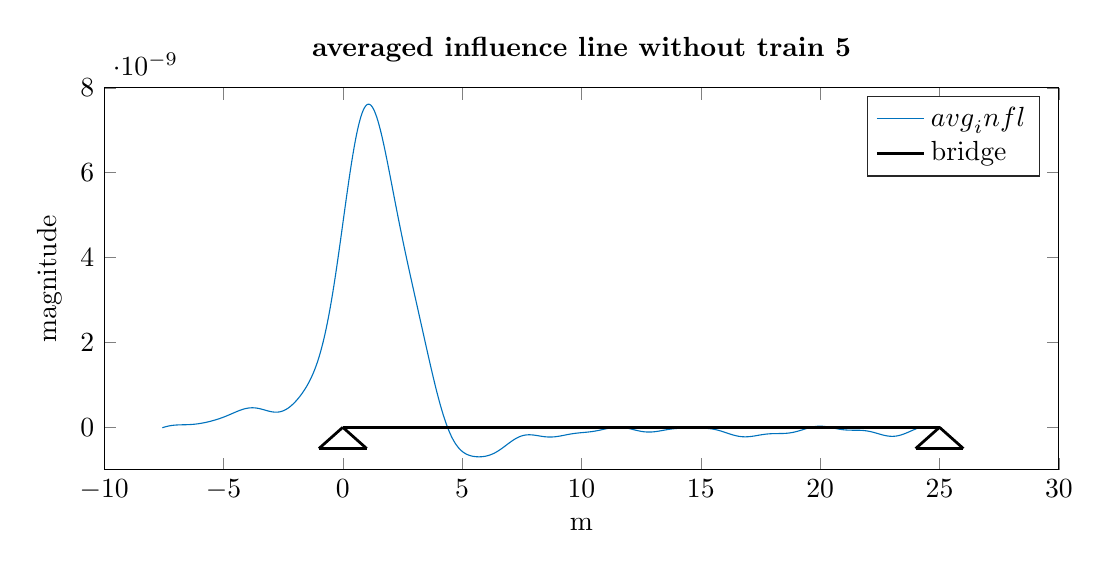
\begin{tikzpicture}

  \begin{axis}[%
    width=\textwidth,
    height=0.4\textwidth,
    at={(0\textwidth,0\textwidth)},
    scale only axis,
    xmin=-10,
    xmax=30,
    xlabel={m},
    ymin=-1e-09,
    ymax=8e-09,
    ylabel={magnitude},
    axis background/.style={fill=white},
    title style={font=\bfseries},
    title={averaged influence line without train 5},
    legend style={legend cell align=left,align=left,draw=white!15!black}
    ]
    \addplot [color=mycolor1,solid]
    table[row sep=crcr]{%
    -7.5590986328125	-1.05355238244679e-11\\
    -7.53894921875	-6.64431757543627e-12\\
    -7.5187998046875	-2.86604271449226e-12\\
    -7.498650390625	7.96300412797682e-13\\
    -7.4785009765625	4.34009158348904e-12\\
    -7.4583515625	7.76309263424537e-12\\
    -7.4382021484375	1.10634481474079e-11\\
    -7.418052734375	1.42396848975327e-11\\
    -7.3979033203125	1.72907100742176e-11\\
    -7.37775390625	2.02158083012966e-11\\
    -7.3576044921875	2.30146374767347e-11\\
    -7.337455078125	2.56872234616078e-11\\
    -7.3173056640625	2.82339536505167e-11\\
    -7.29715625	3.06555694595921e-11\\
    -7.2770068359375	3.29531577718901e-11\\
    -7.256857421875	3.51281413834564e-11\\
    -7.2367080078125	3.71822684965885e-11\\
    -7.21655859375	3.91176013099789e-11\\
    -7.1964091796875	4.09365037582139e-11\\
    -7.176259765625	4.26416284558281e-11\\
    -7.1561103515625	4.42359029035145e-11\\
    -7.1359609375	4.57225150162796e-11\\
    -7.1158115234375	4.71048980352867e-11\\
    -7.095662109375	4.83867148868444e-11\\
    -7.0755126953125	4.9571842053404e-11\\
    -7.05536328125	5.06643530226424e-11\\
    -7.0352138671875	5.16685013816142e-11\\
    -7.015064453125	5.25887036236027e-11\\
    -6.9949150390625	5.34295217356911e-11\\
    -6.974765625	5.41956456351945e-11\\
    -6.9546162109375	5.4891875522936e-11\\
    -6.934466796875	5.55231042209372e-11\\
    -6.9143173828125	5.60942995614179e-11\\
    -6.89416796875	5.6610486893069e-11\\
    -6.8740185546875	5.70767317693558e-11\\
    -6.853869140625	5.74981228821977e-11\\
    -6.8337197265625	5.78797553026579e-11\\
    -6.8135703125	5.82267140884081e-11\\
    -6.7934208984375	5.85440583155477e-11\\
    -6.773271484375	5.8836805590043e-11\\
    -6.7531220703125	5.91099170914767e-11\\
    -6.73297265625	5.93682831990584e-11\\
    -6.7128232421875	5.96167097468747e-11\\
    -6.692673828125	5.98599049523288e-11\\
    -6.6725244140625	6.0102467058368e-11\\
    -6.652375	6.03488727267689e-11\\
    -6.6322255859375	6.06034662161691e-11\\
    -6.612076171875	6.08704493749145e-11\\
    -6.5919267578125	6.11538724750327e-11\\
    -6.57177734375	6.1457625909809e-11\\
    -6.5516279296875	6.17854327735669e-11\\
    -6.531478515625	6.21408423382733e-11\\
    -6.5113291015625	6.25272244376424e-11\\
    -6.4911796875	6.29477647653621e-11\\
    -6.4710302734375	6.34054610901186e-11\\
    -6.450880859375	6.39031203860414e-11\\
    -6.4307314453125	6.44433568732847e-11\\
    -6.41058203125	6.50285909595006e-11\\
    -6.3904326171875	6.56610490691329e-11\\
    -6.370283203125	6.63427643436761e-11\\
    -6.3501337890625	6.70755781923579e-11\\
    -6.329984375	6.78611426691363e-11\\
    -6.3098349609375	6.87009236484345e-11\\
    -6.289685546875	6.95962047687529e-11\\
    -6.2695361328125	7.05480921100888e-11\\
    -6.24938671875	7.15575195681301e-11\\
    -6.2292373046875	7.26252548853409e-11\\
    -6.209087890625	7.37519062964242e-11\\
    -6.1889384765625	7.49379297431899e-11\\
    -6.1687890625	7.61836366116477e-11\\
    -6.1486396484375	7.74892019420825e-11\\
    -6.128490234375	7.88546730611204e-11\\
    -6.1083408203125	8.02799785831826e-11\\
    -6.08819140625	8.17649377274251e-11\\
    -6.0680419921875	8.33092698951829e-11\\
    -6.047892578125	8.49126044520595e-11\\
    -6.0277431640625	8.65744906582739e-11\\
    -6.00759375	8.82944076904943e-11\\
    -5.9874443359375	9.00717746983333e-11\\
    -5.967294921875	9.19059608388535e-11\\
    -5.9471455078125	9.37962952328444e-11\\
    -5.92699609375	9.57420767873425e-11\\
    -5.9068466796875	9.77425838297605e-11\\
    -5.886697265625	9.97970835001926e-11\\
    -5.8665478515625	1.01904840849867e-10\\
    -5.8463984375	1.04065127595371e-10\\
    -5.8262490234375	1.06277230480131e-10\\
    -5.806099609375	1.08540459196762e-10\\
    -5.7859501953125	1.10854153826173e-10\\
    -5.76580078125	1.13217691751831e-10\\
    -5.7456513671875	1.15630494010312e-10\\
    -5.725501953125	1.18092031042088e-10\\
    -5.7053525390625	1.2060182780961e-10\\
    -5.685203125	1.231594682529e-10\\
    -5.6650537109375	1.25764599056215e-10\\
    -5.644904296875	1.28416932702835e-10\\
    -5.6247548828125	1.31116249798588e-10\\
    -5.60460546875	1.33862400648394e-10\\
    -5.5844560546875	1.36655306073911e-10\\
    -5.564306640625	1.39494957464147e-10\\
    -5.5441572265625	1.42381416054795e-10\\
    -5.5240078125	1.45314811435989e-10\\
    -5.5038583984375	1.48295339292034e-10\\
    -5.483708984375	1.5132325838068e-10\\
    -5.4635595703125	1.54398886763338e-10\\
    -5.44341015625	1.57522597301563e-10\\
    -5.4232607421875	1.6069481243894e-10\\
    -5.403111328125	1.63915998291264e-10\\
    -5.3829619140625	1.67186658071583e-10\\
    -5.3628125	1.70507324880249e-10\\
    -5.3426630859375	1.73878553893586e-10\\
    -5.322513671875	1.77300913988106e-10\\
    -5.3023642578125	1.80774978840389e-10\\
    -5.28221484375	1.84301317545786e-10\\
    -5.2620654296875	1.87880484801907e-10\\
    -5.241916015625	1.91513010705586e-10\\
    -5.2217666015625	1.95199390214417e-10\\
    -5.2016171875	1.98940072326243e-10\\
    -5.1814677734375	2.02735449032004e-10\\
    -5.161318359375	2.06585844099145e-10\\
    -5.1411689453125	2.10491501744343e-10\\
    -5.12101953125	2.14452575255632e-10\\
    -5.1008701171875	2.1846911562504e-10\\
    -5.080720703125	2.2254106025366e-10\\
    -5.0605712890625	2.26668221791593e-10\\
    -5.040421875	2.30850277175437e-10\\
    -5.0202724609375	2.35086756926018e-10\\
    -5.000123046875	2.39377034768695e-10\\
    -4.9799736328125	2.43720317638046e-10\\
    -4.95982421875	2.48115636127871e-10\\
    -4.9396748046875	2.52561835446306e-10\\
    -4.919525390625	2.57057566934453e-10\\
    -4.8993759765625	2.61601280205265e-10\\
    -4.8792265625	2.66191215957471e-10\\
    -4.8590771484375	2.70825399517146e-10\\
    -4.838927734375	2.75501635157071e-10\\
    -4.8187783203125	2.80217501241367e-10\\
    -4.79862890625	2.84970346239935e-10\\
    -4.7784794921875	2.89757285654089e-10\\
    -4.758330078125	2.94575199891445e-10\\
    -4.7381806640625	2.99420733124516e-10\\
    -4.71803125	3.04290293163761e-10\\
    -4.6978818359375	3.0918005237189e-10\\
    -4.677732421875	3.1408594964214e-10\\
    -4.6575830078125	3.19003693459053e-10\\
    -4.63743359375	3.23928766055868e-10\\
    -4.6172841796875	3.28856428678241e-10\\
    -4.597134765625	3.33781727959401e-10\\
    -4.5769853515625	3.38699503407248e-10\\
    -4.5568359375	3.43604395999181e-10\\
    -4.5366865234375	3.48490857875723e-10\\
    -4.516537109375	3.53353163119275e-10\\
    -4.4963876953125	3.58185419599532e-10\\
    -4.47623828125	3.62981581862416e-10\\
    -4.4560888671875	3.67735465034622e-10\\
    -4.435939453125	3.72440759711284e-10\\
    -4.4157900390625	3.77091047789657e-10\\
    -4.395640625	3.8167981920727e-10\\
    -4.3754912109375	3.86200489538629e-10\\
    -4.355341796875	3.90646418400333e-10\\
    -4.3351923828125	3.95010928610378e-10\\
    -4.31504296875	3.99287326043532e-10\\
    -4.2948935546875	4.03468920120935e-10\\
    -4.274744140625	4.07549044868564e-10\\
    -4.2545947265625	4.11521080475885e-10\\
    -4.2344453125	4.15378475282987e-10\\
    -4.2142958984375	4.1911476812163e-10\\
    -4.194146484375	4.2272361093312e-10\\
    -4.1739970703125	4.26198791583622e-10\\
    -4.15384765625	4.29534256795549e-10\\
    -4.1336982421875	4.32724135111936e-10\\
    -4.113548828125	4.35762759809372e-10\\
    -4.0933994140625	4.38644691673935e-10\\
    -4.07325	4.41364741553883e-10\\
    -4.0531005859375	4.43917992602377e-10\\
    -4.032951171875	4.46299822123499e-10\\
    -4.0128017578125	4.4850592293502e-10\\
    -3.99265234375	4.50532324162015e-10\\
    -3.9725029296875	4.52375411376348e-10\\
    -3.952353515625	4.54031945998333e-10\\
    -3.9322041015625	4.55499083878517e-10\\
    -3.9120546875	4.56774392979473e-10\\
    -3.8919052734375	4.57855870079826e-10\\
    -3.871755859375	4.58741956425322e-10\\
    -3.8516064453125	4.59431552254753e-10\\
    -3.83145703125	4.59924030131768e-10\\
    -3.8113076171875	4.60219247017222e-10\\
    -3.791158203125	4.60317555020547e-10\\
    -3.7710087890625	4.60219810772814e-10\\
    -3.750859375	4.59927383368551e-10\\
    -3.7307099609375	4.59442160828083e-10\\
    -3.710560546875	4.58766555037081e-10\\
    -3.6904111328125	4.57903505125159e-10\\
    -3.67026171875	4.5685647925067e-10\\
    -3.6501123046875	4.55629474764511e-10\\
    -3.629962890625	4.54227016731315e-10\\
    -3.6098134765625	4.52654154792411e-10\\
    -3.5896640625	4.50916458360853e-10\\
    -3.5695146484375	4.49020010144957e-10\\
    -3.549365234375	4.46971398002992e-10\\
    -3.5292158203125	4.44777705137899e-10\\
    -3.50906640625	4.42446498647262e-10\\
    -3.4889169921875	4.39985816450021e-10\\
    -3.468767578125	4.37404152617803e-10\\
    -3.4486181640625	4.34710441144959e-10\\
    -3.42846875	4.31914038197706e-10\\
    -3.4083193359375	4.29024702888861e-10\\
    -3.388169921875	4.2605257663077e-10\\
    -3.3680205078125	4.23008161124931e-10\\
    -3.34787109375	4.1990229505261e-10\\
    -3.3277216796875	4.16746129536361e-10\\
    -3.307572265625	4.13551102447769e-10\\
    -3.2874228515625	4.10328911641962e-10\\
    -3.2672734375	4.07091487204371e-10\\
    -3.2471240234375	4.03850962799941e-10\\
    -3.226974609375	4.00619646219411e-10\\
    -3.2068251953125	3.97409989221427e-10\\
    -3.18667578125	3.94234556773004e-10\\
    -3.1665263671875	3.91105995794396e-10\\
    -3.146376953125	3.88037003517498e-10\\
    -3.1262275390625	3.85040295569665e-10\\
    -3.106078125	3.82128573897229e-10\\
    -3.0859287109375	3.7931449464492e-10\\
    -3.065779296875	3.76610636109008e-10\\
    -3.0456298828125	3.74029466883106e-10\\
    -3.02548046875	3.71583314316318e-10\\
    -3.0053310546875	3.69284333403663e-10\\
    -2.985181640625	3.67144476228625e-10\\
    -2.9650322265625	3.65175462077017e-10\\
    -2.9448828125	3.63388748340352e-10\\
    -2.9247333984375	3.61795502325406e-10\\
    -2.904583984375	3.60406574084728e-10\\
    -2.8844345703125	3.59232470380475e-10\\
    -2.86428515625	3.58283329891114e-10\\
    -2.8441357421875	3.57568899767296e-10\\
    -2.823986328125	3.57098513639494e-10\\
    -2.8038369140625	3.56881071175901e-10\\
    -2.7836875	3.56925019284555e-10\\
    -2.7635380859375	3.57238335048754e-10\\
    -2.743388671875	3.57828510479482e-10\\
    -2.7232392578125	3.58702539162927e-10\\
    -2.70308984375	3.59866904875112e-10\\
    -2.6829404296875	3.61327572229292e-10\\
    -2.662791015625	3.63089979415093e-10\\
    -2.6426416015625	3.65159033081362e-10\\
    -2.6224921875	3.67539105407426e-10\\
    -2.6023427734375	3.70234033399987e-10\\
    -2.582193359375	3.73247120445051e-10\\
    -2.5620439453125	3.76581140136395e-10\\
    -2.54189453125	3.80238342393937e-10\\
    -2.5217451171875	3.84220461877037e-10\\
    -2.501595703125	3.88528728689426e-10\\
    -2.4814462890625	3.93163881363871e-10\\
    -2.461296875	3.98126182106178e-10\\
    -2.4411474609375	4.03415434269475e-10\\
    -2.420998046875	4.09031002021127e-10\\
    -2.4008486328125	4.14971832156023e-10\\
    -2.38069921875	4.21236478001445e-10\\
    -2.3605498046875	4.27823125350244e-10\\
    -2.340400390625	4.34729620350746e-10\\
    -2.3202509765625	4.41953499273554e-10\\
    -2.3001015625	4.49492020067447e-10\\
    -2.2799521484375	4.57342195608714e-10\\
    -2.259802734375	4.65500828540685e-10\\
    -2.2396533203125	4.73964547592928e-10\\
    -2.21950390625	4.82729845262509e-10\\
    -2.1993544921875	4.91793116733046e-10\\
    -2.179205078125	5.01150699900895e-10\\
    -2.1590556640625	5.10798916371851e-10\\
    -2.13890625	5.20734113286116e-10\\
    -2.1187568359375	5.30952705824173e-10\\
    -2.098607421875	5.41451220241424e-10\\
    -2.0784580078125	5.52226337275245e-10\\
    -2.05830859375	5.63274935764298e-10\\
    -2.0381591796875	5.7459413631672e-10\\
    -2.018009765625	5.86181344860992e-10\\
    -1.9978603515625	5.98034295911173e-10\\
    -1.9777109375	6.10151095376436e-10\\
    -1.9575615234375	6.22530262743814e-10\\
    -1.937412109375	6.35170772462483e-10\\
    -1.9172626953125	6.48072094358013e-10\\
    -1.89711328125	6.61234232905607e-10\\
    -1.8769638671875	6.74657765192628e-10\\
    -1.856814453125	6.8834387740249e-10\\
    -1.8366650390625	7.02294399654458e-10\\
    -1.816515625	7.16511839036844e-10\\
    -1.7963662109375	7.3099941067476e-10\\
    -1.776216796875	7.45761066677706e-10\\
    -1.7560673828125	7.6080152281706e-10\\
    -1.73591796875	7.76126282788839e-10\\
    -1.7157685546875	7.91741659923008e-10\\
    -1.695619140625	8.07654796206972e-10\\
    -1.6754697265625	8.23873678497891e-10\\
    -1.6553203125	8.40407151805859e-10\\
    -1.6351708984375	8.57264929537944e-10\\
    -1.615021484375	8.74457600601497e-10\\
    -1.5948720703125	8.91996633273958e-10\\
    -1.57472265625	9.09894375755699e-10\\
    -1.5545732421875	9.2816405333207e-10\\
    -1.534423828125	9.46819762080853e-10\\
    -1.5142744140625	9.65876459071714e-10\\
    -1.494125	9.85349949014905e-10\\
    -1.4739755859375	1.0052568673274e-09\\
    -1.453826171875	1.02561465959589e-09\\
    -1.4336767578125	1.04644155742737e-09\\
    -1.41352734375	1.0677565506898e-09\\
    -1.3933779296875	1.08957935615678e-09\\
    -1.373228515625	1.11193038258228e-09\\
    -1.3530791015625	1.13483069224302e-09\\
    -1.3329296875	1.15830195899842e-09\\
    -1.3127802734375	1.18236642292937e-09\\
    -1.292630859375	1.20704684162957e-09\\
    -1.2724814453125	1.23236643823432e-09\\
    -1.25233203125	1.25834884628366e-09\\
    -1.2321826171875	1.28501805152811e-09\\
    -1.212033203125	1.31239833079646e-09\\
    -1.1918837890625	1.34051418805609e-09\\
    -1.171734375	1.36939028780713e-09\\
    -1.1515849609375	1.39905138596196e-09\\
    -1.131435546875	1.42952225837191e-09\\
    -1.1112861328125	1.46082762717236e-09\\
    -1.09113671875	1.49299208512694e-09\\
    -1.0709873046875	1.52604001816026e-09\\
    -1.050837890625	1.55999552627674e-09\\
    -1.0306884765625	1.59488234307114e-09\\
    -1.0105390625	1.63072375404342e-09\\
    -0.9903896484375	1.66754251393735e-09\\
    -0.970240234374999	1.70536076332824e-09\\
    -0.950090820312499	1.74419994469066e-09\\
    -0.929941406249999	1.78408071818175e-09\\
    -0.9097919921875	1.82502287737987e-09\\
    -0.889642578124999	1.86704526522164e-09\\
    -0.869493164062499	1.91016569038337e-09\\
    -0.849343749999999	1.95440084435456e-09\\
    -0.829194335937499	1.99976621945261e-09\\
    -0.809044921875	2.04627602802837e-09\\
    -0.788895507812499	2.09394312311187e-09\\
    -0.768746093749999	2.1427789207466e-09\\
    -0.748596679687499	2.19279332425889e-09\\
    -0.728447265624999	2.24399465070655e-09\\
    -0.7082978515625	2.29638955974762e-09\\
    -0.688148437499999	2.34998298516582e-09\\
    -0.667999023437499	2.40477806928498e-09\\
    -0.647849609374999	2.46077610049868e-09\\
    -0.627700195312499	2.51797645413548e-09\\
    -0.60755078125	2.57637653687293e-09\\
    -0.587401367187499	2.63597173490601e-09\\
    -0.567251953124999	2.69675536606721e-09\\
    -0.547102539062499	2.75871863608651e-09\\
    -0.526953124999999	2.82185059916987e-09\\
    -0.5068037109375	2.88613812306452e-09\\
    -0.486654296874999	2.95156585876858e-09\\
    -0.466504882812499	3.0181162150311e-09\\
    -0.446355468749999	3.08576933777657e-09\\
    -0.4262060546875	3.15450309457572e-09\\
    -0.406056640625	3.22429306427139e-09\\
    -0.385907226562499	3.29511253185496e-09\\
    -0.365757812499999	3.36693248867517e-09\\
    -0.345608398437499	3.43972163804699e-09\\
    -0.325458984375	3.51344640631411e-09\\
    -0.305309570312499	3.58807095940353e-09\\
    -0.285160156249999	3.66355722489642e-09\\
    -0.265010742187499	3.7398649196239e-09\\
    -0.244861328124999	3.81695158278154e-09\\
    -0.2247119140625	3.8947726145409e-09\\
    -0.204562499999999	3.97328132012131e-09\\
    -0.184413085937499	4.05242895926954e-09\\
    -0.164263671874999	4.13216480107994e-09\\
    -0.144114257812499	4.21243618407228e-09\\
    -0.12396484375	4.29318858142967e-09\\
    -0.103815429687499	4.37436567128368e-09\\
    -0.0836660156249991	4.45590941191976e-09\\
    -0.0635166015624993	4.53776012176093e-09\\
    -0.0433671874999995	4.61985656397431e-09\\
    -0.0232177734374996	4.70213603553091e-09\\
    -0.00306835937499894	4.78453446053613e-09\\
    0.0170810546875009	4.86698648763519e-09\\
    0.0372304687500007	4.94942559128578e-09\\
    0.0573798828125005	5.03178417667789e-09\\
    0.0775292968750003	5.11399368807e-09\\
    0.097678710937501	5.19598472029957e-09\\
    0.117828125000001	5.27768713321618e-09\\
    0.137977539062501	5.35903016877597e-09\\
    0.158126953125	5.43994257052741e-09\\
    0.178276367187501	5.52035270521051e-09\\
    0.198425781250001	5.60018868618414e-09\\
    0.218575195312501	5.67937849838999e-09\\
    0.238724609375001	5.75785012455568e-09\\
    0.2588740234375	5.83553167233488e-09\\
    0.279023437500001	5.91235150207825e-09\\
    0.299172851562501	5.98823835492586e-09\\
    0.319322265625001	6.06312148090923e-09\\
    0.339471679687501	6.13693076675009e-09\\
    0.35962109375	6.20959686304194e-09\\
    0.379770507812501	6.28105131050112e-09\\
    0.399919921875001	6.35122666497517e-09\\
    0.420069335937501	6.42005662089843e-09\\
    0.440218750000001	6.48747613288759e-09\\
    0.4603681640625	6.55342153517402e-09\\
    0.480517578125	6.61783065857418e-09\\
    0.5006669921875	6.68064294470509e-09\\
    0.520816406250002	6.74179955715811e-09\\
    0.540965820312501	6.80124348935175e-09\\
    0.561115234375001	6.85891966879182e-09\\
    0.581264648437501	6.91477505747653e-09\\
    0.601414062500001	6.9687587481933e-09\\
    0.621563476562501	7.02082205646462e-09\\
    0.641712890625	7.07091860791103e-09\\
    0.6618623046875	7.1190044208112e-09\\
    0.68201171875	7.16503798365133e-09\\
    0.7021611328125	7.20898032746885e-09\\
    0.722310546875002	7.25079509280899e-09\\
    0.742459960937501	7.29044859112706e-09\\
    0.762609375000001	7.32790986048311e-09\\
    0.782758789062501	7.36315071539137e-09\\
    0.802908203125001	7.39614579070164e-09\\
    0.823057617187501	7.42687257940581e-09\\
    0.84320703125	7.45531146427855e-09\\
    0.8633564453125	7.48144574327771e-09\\
    0.883505859375	7.50526164864616e-09\\
    0.9036552734375	7.5267483596739e-09\\
    0.923804687500001	7.54589800909572e-09\\
    0.943954101562501	7.56270568311665e-09\\
    0.964103515625001	7.5771694150747e-09\\
    0.984252929687501	7.58929017276662e-09\\
    1.00440234375	7.59907183947992e-09\\
    1.0245517578125	7.60652118879055e-09\\
    1.044701171875	7.61164785320242e-09\\
    1.0648505859375	7.61446428672129e-09\\
    1.085	7.61498572147124e-09\\
    1.1051494140625	7.6132301184782e-09\\
    1.125298828125	7.6092181127598e-09\\
    1.1454482421875	7.60297295287616e-09\\
    1.16559765625	7.59452043511053e-09\\
    1.1857470703125	7.58388883246286e-09\\
    1.205896484375	7.57110881865261e-09\\
    1.2260458984375	7.55621338734029e-09\\
    1.2461953125	7.53923776678937e-09\\
    1.2663447265625	7.52021933020179e-09\\
    1.286494140625	7.49919750197146e-09\\
    1.3066435546875	7.47621366011023e-09\\
    1.32679296875	7.45131103511045e-09\\
    1.3469423828125	7.42453460551685e-09\\
    1.367091796875	7.39593099048861e-09\\
    1.3872412109375	7.36554833963957e-09\\
    1.407390625	7.33343622045073e-09\\
    1.4275400390625	7.29964550355487e-09\\
    1.447689453125	7.26422824619755e-09\\
    1.4678388671875	7.22723757418255e-09\\
    1.48798828125	7.18872756261257e-09\\
    1.5081376953125	7.14875311573809e-09\\
    1.528287109375	7.10736984622816e-09\\
    1.5484365234375	7.06463395417714e-09\\
    1.5685859375	7.02060210616064e-09\\
    1.5887353515625	6.97533131465222e-09\\
    1.608884765625	6.92887881810988e-09\\
    1.6290341796875	6.88130196203801e-09\\
    1.64918359375	6.83265808132606e-09\\
    1.6693330078125	6.78300438416027e-09\\
    1.689482421875	6.73239783779856e-09\\
    1.7096318359375	6.68089505649217e-09\\
    1.72978125	6.62855219182982e-09\\
    1.7499306640625	6.57542482577212e-09\\
    1.770080078125	6.52156786663451e-09\\
    1.7902294921875	6.46703544826757e-09\\
    1.81037890625	6.41188083267295e-09\\
    1.8305283203125	6.35615631628187e-09\\
    1.850677734375	6.29991314011187e-09\\
    1.8708271484375	6.24320140400466e-09\\
    1.8909765625	6.18606998513549e-09\\
    1.9111259765625	6.12856646097108e-09\\
    1.931275390625	6.07073703683911e-09\\
    1.9514248046875	6.01262647825845e-09\\
    1.97157421875	5.95427804816453e-09\\
    1.9917236328125	5.89573344914949e-09\\
    2.011873046875	5.83703277082143e-09\\
    2.0320224609375	5.77821444237211e-09\\
    2.052171875	5.7193151904263e-09\\
    2.0723212890625	5.66037000223096e-09\\
    2.092470703125	5.60141209422604e-09\\
    2.1126201171875	5.54247288602342e-09\\
    2.13276953125	5.48358197980427e-09\\
    2.1529189453125	5.42476714512972e-09\\
    2.173068359375	5.36605430914387e-09\\
    2.1932177734375	5.30746755213278e-09\\
    2.2133671875	5.24902910838785e-09\\
    2.2335166015625	5.19075937230681e-09\\
    2.253666015625	5.13267690965105e-09\\
    2.2738154296875	5.07479847386325e-09\\
    2.29396484375	5.01713902733569e-09\\
    2.3141142578125	4.95971176750549e-09\\
    2.334263671875	4.90252815764033e-09\\
    2.3544130859375	4.84559796216524e-09\\
    2.3745625	4.78892928636904e-09\\
    2.3947119140625	4.73252862031733e-09\\
    2.414861328125	4.6764008867881e-09\\
    2.4350107421875	4.62054949303557e-09\\
    2.45516015625	4.56497638617826e-09\\
    2.4753095703125	4.50968211199815e-09\\
    2.495458984375	4.45466587692966e-09\\
    2.5156083984375	4.39992561300955e-09\\
    2.5357578125	4.34545804555193e-09\\
    2.5559072265625	4.29125876330661e-09\\
    2.576056640625	4.23732229085386e-09\\
    2.5962060546875	4.18364216298375e-09\\
    2.61635546875	4.13021100080521e-09\\
    2.6365048828125	4.07702058932642e-09\\
    2.656654296875	4.02406195624657e-09\\
    2.6768037109375	3.97132545169753e-09\\
    2.696953125	3.91880082867366e-09\\
    2.7171025390625	3.86647732388829e-09\\
    2.737251953125	3.81434373879673e-09\\
    2.7574013671875	3.76238852052749e-09\\
    2.77755078125	3.71059984246628e-09\\
    2.7977001953125	3.65896568424093e-09\\
    2.817849609375	3.60747391085946e-09\\
    2.8379990234375	3.55611235075898e-09\\
    2.8581484375	3.50486887252836e-09\\
    2.8782978515625	3.45373146007454e-09\\
    2.898447265625	3.40268828600914e-09\\
    2.9185966796875	3.35172778303997e-09\\
    2.93874609375	3.30083871316036e-09\\
    2.9588955078125	3.2500102344384e-09\\
    2.979044921875	3.19923196521724e-09\\
    2.9991943359375	3.14849404554835e-09\\
    3.01934375	3.09778719568945e-09\\
    3.0394931640625	3.04710277151041e-09\\
    3.059642578125	2.99643281666132e-09\\
    3.0797919921875	2.94577011136921e-09\\
    3.09994140625	2.89510821774138e-09\\
    3.1200908203125	2.84444152146642e-09\\
    3.140240234375	2.79376526981585e-09\\
    3.1603896484375	2.74307560586297e-09\\
    3.1805390625	2.69236959884773e-09\\
    3.2006884765625	2.64164527063025e-09\\
    3.220837890625	2.59090161818836e-09\\
    3.2409873046875	2.54013863212808e-09\\
    3.26113671875	2.48935731118892e-09\\
    3.2812861328125	2.43855967273943e-09\\
    3.301435546875	2.38774875927122e-09\\
    3.3215849609375	2.33692864091278e-09\\
    3.341734375	2.28610441399719e-09\\
    3.3618837890625	2.23528219573056e-09\\
    3.382033203125	2.18446911501999e-09\\
    3.4021826171875	2.13367329953229e-09\\
    3.42233203125	2.08290385906616e-09\\
    3.4424814453125	2.03217086533196e-09\\
    3.462630859375	1.98148532824408e-09\\
    3.4827802734375	1.93085916884157e-09\\
    3.5029296875	1.88030518896259e-09\\
    3.5230791015625	1.82983703780783e-09\\
    3.543228515625	1.77946917553715e-09\\
    3.5633779296875	1.72921683405221e-09\\
    3.58352734375	1.67909597512556e-09\\
    3.6036767578125	1.62912324604422e-09\\
    3.623826171875	1.57931593294244e-09\\
    3.6439755859375	1.52969191200433e-09\\
    3.664125	1.48026959872255e-09\\
    3.6842744140625	1.43106789540399e-09\\
    3.704423828125	1.38210613711759e-09\\
    3.7245732421875	1.33340403628275e-09\\
    3.74472265625	1.28498162609944e-09\\
    3.7648720703125	1.23685920302356e-09\\
    3.785021484375	1.18905726849199e-09\\
    3.8051708984375	1.14159647010268e-09\\
    3.8253203125	1.09449754245516e-09\\
    3.8454697265625	1.04778124785603e-09\\
    3.865619140625	1.0014683170926e-09\\
    3.8857685546875	9.55579390475888e-10\\
    3.90591796875	9.10134959351497e-10\\
    3.9260673828125	8.65155308273366e-10\\
    3.946216796875	8.20660458031666e-10\\
    3.9663662109375	7.76670109721348e-10\\
    3.986515625	7.33203590032774e-10\\
    4.0066650390625	6.90279797940077e-10\\
    4.026814453125	6.47917152956648e-10\\
    4.0469638671875	6.06133545120347e-10\\
    4.06711328125	5.64946286863715e-10\\
    4.0872626953125	5.24372066916737e-10\\
    4.107412109375	4.84426906381505e-10\\
    4.1275615234375	4.45126117109526e-10\\
    4.1477109375	4.06484262503454e-10\\
    4.1678603515625	3.68515120855736e-10\\
    4.188009765625	3.31231651327011e-10\\
    4.2081591796875	2.94645962657235e-10\\
    4.22830859375	2.58769284692404e-10\\
    4.2484580078125	2.23611942799372e-10\\
    4.268607421875	1.89183335230835e-10\\
    4.2887568359375	1.55491913491887e-10\\
    4.30890625	1.22545165748894e-10\\
    4.3290556640625	9.03496033106592e-11\\
    4.349205078125	5.89107502010597e-11\\
    4.3693544921875	2.82331358316446e-11\\
    4.38950390625	-1.67970922809045e-12\\
    4.4096533203125	-3.08252543955456e-11\\
    4.429802734375	-5.92019671583242e-11\\
    4.4499521484375	-8.68093081296009e-11\\
    4.4701015625	-1.1364772311928e-10\\
    4.4902509765625	-1.39718632274548e-10\\
    4.510400390625	-1.65024416353047e-10\\
    4.5305498046875	-1.89568400201184e-10\\
    4.55069921875	-2.13354833519137e-10\\
    4.5708486328125	-2.36388869002718e-10\\
    4.590998046875	-2.58676537960537e-10\\
    4.6111474609375	-2.80224723512767e-10\\
    4.631296875	-3.01041131485243e-10\\
    4.6514462890625	-3.21134259119571e-10\\
    4.671595703125	-3.40513361726479e-10\\
    4.6917451171875	-3.59188417415611e-10\\
    4.71189453125	-3.77170090040456e-10\\
    4.7320439453125	-3.94469690502129e-10\\
    4.752193359375	-4.11099136560102e-10\\
    4.7723427734375	-4.27070911301896e-10\\
    4.7924921875	-4.42398020427066e-10\\
    4.8126416015625	-4.57093948503564e-10\\
    4.832791015625	-4.71172614356759e-10\\
    4.8529404296875	-4.84648325752976e-10\\
    4.87308984375	-4.97535733540484e-10\\
    4.8932392578125	-5.09849785411271e-10\\
    4.913388671875	-5.21605679446859e-10\\
    4.9335380859375	-5.32818817610673e-10\\
    4.9536875	-5.43504759348267e-10\\
    4.9738369140625	-5.53679175454842e-10\\
    4.993986328125	-5.6335780236717e-10\\
    5.0141357421875	-5.72556397034107e-10\\
    5.03428515625	-5.81290692516479e-10\\
    5.0544345703125	-5.89576354463202e-10\\
    5.074583984375	-5.97428938606054e-10\\
    5.0947333984375	-6.04863849410685e-10\\
    5.1148828125	-6.11896300016086e-10\\
    5.1350322265625	-6.18541273588978e-10\\
    5.155181640625	-6.24813486213453e-10\\
    5.1753310546875	-6.30727351429615e-10\\
    5.19548046875	-6.36296946528121e-10\\
    5.2156298828125	-6.41535980700247e-10\\
    5.235779296875	-6.46457765135631e-10\\
    5.2559287109375	-6.51075185152018e-10\\
    5.276078125	-6.55400674433312e-10\\
    5.2962275390625	-6.59446191443981e-10\\
    5.316376953125	-6.63223198079438e-10\\
    5.3365263671875	-6.66742640603461e-10\\
    5.35667578125	-6.70014932914957e-10\\
    5.3768251953125	-6.73049942177667e-10\\
    5.396974609375	-6.75856976837491e-10\\
    5.4171240234375	-6.78444777043314e-10\\
    5.4372734375	-6.80821507478287e-10\\
    5.4574228515625	-6.82994752599753e-10\\
    5.477572265625	-6.84971514277226e-10\\
    5.4977216796875	-6.8675821180919e-10\\
    5.51787109375	-6.88360684290961e-10\\
    5.5380205078125	-6.89784195297498e-10\\
    5.558169921875	-6.91033439836888e-10\\
    5.5783193359375	-6.92112553522257e-10\\
    5.59846875	-6.93025123902159e-10\\
    5.6186181640625	-6.93774203882071e-10\\
    5.638767578125	-6.94362327162441e-10\\
    5.6589169921875	-6.94791525611942e-10\\
    5.67906640625	-6.95063348488079e-10\\
    5.6992158203125	-6.95178883411195e-10\\
    5.719365234375	-6.95138778992136e-10\\
    5.7395146484375	-6.94943269008541e-10\\
    5.7596640625	-6.94592198019788e-10\\
    5.7798134765625	-6.94085048306074e-10\\
    5.799962890625	-6.93420968013165e-10\\
    5.8201123046875	-6.92598800380649e-10\\
    5.84026171875	-6.91617113928482e-10\\
    5.8604111328125	-6.90474233473928e-10\\
    5.880560546875	-6.89168271848834e-10\\
    5.9007099609375	-6.8769716218551e-10\\
    5.920859375	-6.86058690638282e-10\\
    5.9410087890625	-6.84250529407122e-10\\
    5.961158203125	-6.82270269929483e-10\\
    5.9813076171875	-6.80115456106864e-10\\
    6.00145703125	-6.77783617433275e-10\\
    6.0216064453125	-6.75272301894121e-10\\
    6.041755859375	-6.72579108505704e-10\\
    6.0619052734375	-6.69701719367733e-10\\
    6.0820546875	-6.66637931103876e-10\\
    6.1022041015625	-6.63385685568484e-10\\
    6.122353515625	-6.59943099701117e-10\\
    6.1425029296875	-6.56308494414417e-10\\
    6.16265234375	-6.52480422405222e-10\\
    6.1828017578125	-6.48457694783498e-10\\
    6.202951171875	-6.44239406418706e-10\\
    6.2231005859375	-6.39824959908675e-10\\
    6.24325	-6.35214088081715e-10\\
    6.2633994140625	-6.30406874948739e-10\\
    6.283548828125	-6.25403775028474e-10\\
    6.3036982421875	-6.20205630975317e-10\\
    6.32384765625	-6.1481368944621e-10\\
    6.3439970703125	-6.09229615149845e-10\\
    6.364146484375	-6.03455503028598e-10\\
    6.3842958984375	-5.97493888530941e-10\\
    6.4044453125	-5.91347755939391e-10\\
    6.4245947265625	-5.85020544726597e-10\\
    6.444744140625	-5.78516153919678e-10\\
    6.4648935546875	-5.71838944460507e-10\\
    6.48504296875	-5.6499373955723e-10\\
    6.5051923828125	-5.57985823029882e-10\\
    6.525341796875	-5.50820935660457e-10\\
    6.5454912109375	-5.4350526956526e-10\\
    6.565640625	-5.36045460614699e-10\\
    6.5857900390625	-5.28448578932898e-10\\
    6.605939453125	-5.20722117516569e-10\\
    6.6260888671875	-5.12873979019476e-10\\
    6.64623828125	-5.04912460755509e-10\\
    6.6663876953125	-4.96846237979836e-10\\
    6.686537109375	-4.88684345513825e-10\\
    6.7066865234375	-4.80436157785367e-10\\
    6.7268359375	-4.72111367361892e-10\\
    6.7469853515625	-4.637199620587e-10\\
    6.767134765625	-4.55272200710272e-10\\
    6.7872841796875	-4.46778587696889e-10\\
    6.80743359375	-4.38249846323215e-10\\
    6.8275830078125	-4.29696891149429e-10\\
    6.847732421875	-4.2113079937909e-10\\
    6.8678818359375	-4.12562781411032e-10\\
    6.88803125	-4.04004150665413e-10\\
    6.9081806640625	-3.95466292796309e-10\\
    6.928330078125	-3.86960634405251e-10\\
    6.9484794921875	-3.78498611371533e-10\\
    6.96862890625	-3.70091636916236e-10\\
    6.9887783203125	-3.61751069517535e-10\\
    7.008927734375	-3.53488180795052e-10\\
    7.0290771484375	-3.45314123480822e-10\\
    7.0492265625	-3.37239899593758e-10\\
    7.0693759765625	-3.29276328933448e-10\\
    7.089525390625	-3.21434018007615e-10\\
    7.1096748046875	-3.13723329505666e-10\\
    7.12982421875	-3.06154352428461e-10\\
    7.1499736328125	-2.9873687298171e-10\\
    7.170123046875	-2.91480346337371e-10\\
    7.1902724609375	-2.84393869363928e-10\\
    7.210421875	-2.77486154422671e-10\\
    7.2305712890625	-2.70765504322926e-10\\
    7.250720703125	-2.64239788524763e-10\\
    7.2708701171875	-2.57916420672906e-10\\
    7.29101953125	-2.51802337540561e-10\\
    7.3111689453125	-2.45903979456513e-10\\
    7.331318359375	-2.40227272283349e-10\\
    7.3514677734375	-2.34777611008809e-10\\
    7.3716171875	-2.29559845006324e-10\\
    7.3917666015625	-2.24578265014626e-10\\
    7.411916015625	-2.19836591879969e-10\\
    7.4320654296875	-2.15337967098072e-10\\
    7.45221484375	-2.11084945186295e-10\\
    7.4723642578125	-2.07079487909949e-10\\
    7.492513671875	-2.03322960379867e-10\\
    7.5126630859375	-1.99816129031698e-10\\
    7.5328125	-1.96559161490531e-10\\
    7.5529619140625	-1.93551628317789e-10\\
    7.573111328125	-1.90792506630578e-10\\
    7.5932607421875	-1.88280185577049e-10\\
    7.61341015625	-1.86012473644756e-10\\
    7.6335595703125	-1.83986607772554e-10\\
    7.653708984375	-1.82199264230253e-10\\
    7.6738583984375	-1.80646571224078e-10\\
    7.6940078125	-1.79324123179997e-10\\
    7.7141572265625	-1.782269966512e-10\\
    7.734306640625	-1.77349767790395e-10\\
    7.7544560546875	-1.7668653132232e-10\\
    7.77460546875	-1.76230920946702e-10\\
    7.7947548828125	-1.75976131097159e-10\\
    7.814904296875	-1.75914939976974e-10\\
    7.8350537109375	-1.76039733788461e-10\\
    7.855203125	-1.76342532068759e-10\\
    7.8753525390625	-1.76815014041301e-10\\
    7.895501953125	-1.77448545888982e-10\\
    7.9156513671875	-1.78234208852208e-10\\
    7.93580078125	-1.79162828052421e-10\\
    7.9559501953125	-1.80225001939654e-10\\
    7.976099609375	-1.81411132260808e-10\\
    7.9962490234375	-1.82711454444016e-10\\
    8.0163984375	-1.84116068293427e-10\\
    8.0365478515625	-1.85614968888141e-10\\
    8.056697265625	-1.87198077578788e-10\\
    8.0768466796875	-1.88855272975378e-10\\
    8.09699609375	-1.90576421820645e-10\\
    8.1171455078125	-1.92351409643945e-10\\
    8.137294921875	-1.94170171092128e-10\\
    8.1574443359375	-1.96022719835433e-10\\
    8.17759375	-1.97899177948476e-10\\
    8.1977431640625	-1.99789804668785e-10\\
    8.217892578125	-2.0168502443805e-10\\
    8.2380419921875	-2.03575454134287e-10\\
    8.25819140625	-2.05451929406509e-10\\
    8.2783408203125	-2.07305530027135e-10\\
    8.298490234375	-2.0912760418133e-10\\
    8.3186396484375	-2.10909791616745e-10\\
    8.3387890625	-2.12644045581521e-10\\
    8.3589384765625	-2.14322653483279e-10\\
    8.379087890625	-2.15938256206639e-10\\
    8.3992373046875	-2.17483866032067e-10\\
    8.41938671875	-2.1895288310412e-10\\
    8.4395361328125	-2.20339110402695e-10\\
    8.459685546875	-2.21636767176517e-10\\
    8.4798349609375	-2.22840500803859e-10\\
    8.499984375	-2.23945397051349e-10\\
    8.5201337890625	-2.24946988707676e-10\\
    8.540283203125	-2.25841262574977e-10\\
    8.5604326171875	-2.2662466480671e-10\\
    8.58058203125	-2.27294104586896e-10\\
    8.6007314453125	-2.27846956151585e-10\\
    8.620880859375	-2.28281059159444e-10\\
    8.6410302734375	-2.28594717424247e-10\\
    8.6611796875	-2.28786696027987e-10\\
    8.6813291015625	-2.28856216838995e-10\\
    8.701478515625	-2.28802952465194e-10\\
    8.7216279296875	-2.28627018678037e-10\\
    8.74177734375	-2.28328965348102e-10\\
    8.7619267578125	-2.27909765938415e-10\\
    8.782076171875	-2.2737080560661e-10\\
    8.8022255859375	-2.26713867971759e-10\\
    8.822375	-2.25941120606245e-10\\
    8.8425244140625	-2.25055099317352e-10\\
    8.862673828125	-2.24058691287261e-10\\
    8.8828232421875	-2.22955117143896e-10\\
    8.90297265625	-2.21747912038532e-10\\
    8.9231220703125	-2.2044090580927e-10\\
    8.943271484375	-2.19038202312294e-10\\
    8.9634208984375	-2.17544158005435e-10\\
    8.9835703125	-2.15963359870731e-10\\
    9.0037197265625	-2.14300602764591e-10\\
    9.023869140625	-2.12560866285719e-10\\
    9.0440185546875	-2.10749291252133e-10\\
    9.06416796875	-2.08871155879531e-10\\
    9.0843173828125	-2.06931851753706e-10\\
    9.104466796875	-2.04936859689932e-10\\
    9.1246162109375	-2.02891725572054e-10\\
    9.144765625	-2.00802036263472e-10\\
    9.1649150390625	-1.98673395681367e-10\\
    9.185064453125	-1.96511401124321e-10\\
    9.2052138671875	-1.94321619941947e-10\\
    9.22536328125	-1.92109566633278e-10\\
    9.2455126953125	-1.89880680458531e-10\\
    9.265662109375	-1.8764030364637e-10\\
    9.2858115234375	-1.85393660276015e-10\\
    9.3059609375	-1.83145835910506e-10\\
    9.3261103515625	-1.80901758054125e-10\\
    9.346259765625	-1.78666177503356e-10\\
    9.3664091796875	-1.76443650656976e-10\\
    9.38655859375	-1.7423852284681e-10\\
    9.4067080078125	-1.72054912746415e-10\\
    9.426857421875	-1.69896697910498e-10\\
    9.4470068359375	-1.67767501493233e-10\\
    9.46715625	-1.65670680188879e-10\\
    9.4873056640625	-1.63609313433102e-10\\
    9.507455078125	-1.61586193898404e-10\\
    9.5276044921875	-1.59603819311856e-10\\
    9.54775390625	-1.57664385618118e-10\\
    9.5679033203125	-1.55769781505391e-10\\
    9.588052734375	-1.53921584306605e-10\\
    9.6082021484375	-1.52121057282793e-10\\
    9.6283515625	-1.5036914829016e-10\\
    9.6485009765625	-1.4866648982708e-10\\
    9.668650390625	-1.47013400451839e-10\\
    9.6887998046875	-1.45409887556762e-10\\
    9.70894921875	-1.4385565147909e-10\\
    9.7290986328125	-1.42350090923938e-10\\
    9.749248046875	-1.40892309669659e-10\\
    9.7693974609375	-1.39481124521085e-10\\
    9.789546875	-1.38115074471439e-10\\
    9.8096962890625	-1.36792431029162e-10\\
    9.829845703125	-1.35511209661571e-10\\
    9.8499951171875	-1.34269182303093e-10\\
    9.87014453125	-1.33063890871932e-10\\
    9.8902939453125	-1.31892661735261e-10\\
    9.910443359375	-1.30752621059638e-10\\
    9.9305927734375	-1.29640710980077e-10\\
    9.9507421875	-1.28553706518303e-10\\
    9.9708916015625	-1.27488233178052e-10\\
    9.991041015625	-1.26440785142847e-10\\
    10.0111904296875	-1.25407743999665e-10\\
    10.03133984375	-1.24385397910061e-10\\
    10.0514892578125	-1.23369961148857e-10\\
    10.071638671875	-1.22357593929311e-10\\
    10.0917880859375	-1.21344422432849e-10\\
    10.1119375	-1.20326558960855e-10\\
    10.1320869140625	-1.19300122125819e-10\\
    10.152236328125	-1.18261256999219e-10\\
    10.1723857421875	-1.17206155133893e-10\\
    10.19253515625	-1.16131074379418e-10\\
    10.2126845703125	-1.15032358409974e-10\\
    10.232833984375	-1.1390645588558e-10\\
    10.2529833984375	-1.12749939169118e-10\\
    10.2731328125	-1.11559522523584e-10\\
    10.2932822265625	-1.1033207971611e-10\\
    10.313431640625	-1.09064660957849e-10\\
    10.3335810546875	-1.07754509111521e-10\\
    10.35373046875	-1.06399075101425e-10\\
    10.3738798828125	-1.04996032463937e-10\\
    10.394029296875	-1.03543290980015e-10\\
    10.4141787109375	-1.02039009334882e-10\\
    10.434328125	-1.00481606753933e-10\\
    10.4544775390625	-9.88697735680105e-11\\
    10.474626953125	-9.72024806653877e-11\\
    10.4947763671875	-9.547898779223e-11\\
    10.51492578125	-9.36988506677625e-11\\
    10.5350751953125	-9.18619268851053e-11\\
    10.555224609375	-8.99683805733968e-11\\
    10.5753740234375	-8.80186858017056e-11\\
    10.5955234375	-8.60136287101001e-11\\
    10.6156728515625	-8.39543083581989e-11\\
    10.635822265625	-8.18421362864685e-11\\
    10.6559716796875	-7.96788347905314e-11\\
    10.67612109375	-7.74664339136927e-11\\
    10.6962705078125	-7.52072671678575e-11\\
    10.716419921875	-7.2903965997853e-11\\
    10.7365693359375	-7.05594530090394e-11\\
    10.75671875	-6.81769339828148e-11\\
    10.7768681640625	-6.57598887092308e-11\\
    10.797017578125	-6.33120606705179e-11\\
    10.8171669921875	-6.08374456136352e-11\\
    10.83731640625	-5.83402790542408e-11\\
    10.8574658203125	-5.58250227585299e-11\\
    10.877615234375	-5.32963502532679e-11\\
    10.8977646484375	-5.07591314180427e-11\\
    10.9179140625	-4.82184162172445e-11\\
    10.9380634765625	-4.5679417632522e-11\\
    10.958212890625	-4.31474938595017e-11\\
    10.9783623046875	-4.06281298353493e-11\\
    10.99851171875	-3.81269181662281e-11\\
    11.0186611328125	-3.56495395260449e-11\\
    11.038810546875	-3.32017425997816e-11\\
    11.0589599609375	-3.07893236464931e-11\\
    11.079109375	-2.8418105758434e-11\\
    11.0992587890625	-2.60939178939209e-11\\
    11.119408203125	-2.38225737624088e-11\\
    11.1395576171875	-2.16098506407683e-11\\
    11.15970703125	-1.94614682000397e-11\\
    11.1798564453125	-1.73830674218566e-11\\
    11.200005859375	-1.53801896834377e-11\\
    11.2201552734375	-1.34582560893548e-11\\
    11.2403046875	-1.16225471274047e-11\\
    11.2604541015625	-9.87818272465071e-12\\
    11.280603515625	-8.23010277824696e-12\\
    11.3007529296875	-6.68304823383198e-12\\
    11.32090234375	-5.24154278228244e-12\\
    11.3410517578125	-3.90987524325606e-12\\
    11.361201171875	-2.69208270144742e-12\\
    11.3813505859375	-1.59193445863598e-12\\
    11.4015	-6.12916861583759e-13\\
    11.4216494140625	2.41780937394482e-13\\
    11.441798828125	9.69280233870953e-13\\
    11.4619482421875	1.56702498904161e-12\\
    11.48209765625	2.03279296591549e-12\\
    11.5022470703125	2.36470574211149e-12\\
    11.522396484375	2.56123756155177e-12\\
    11.5425458984375	2.62122299164337e-12\\
    11.5626953125	2.54386335693125e-12\\
    11.5828447265625	2.32873192472349e-12\\
    11.602994140625	1.97577782276783e-12\\
    11.6231435546875	1.48532867373148e-12\\
    11.64329296875	8.58091935925804e-13\\
    11.6634423828125	9.51549444733493e-14\\
    11.683591796875	-8.020163481424e-13\\
    11.7037412109375	-1.83157992842568e-12\\
    11.723890625	-2.99132156671685e-12\\
    11.7440400390625	-4.27865993738459e-12\\
    11.764189453125	-5.69065299662158e-12\\
    11.7843388671875	-7.22400559550211e-12\\
    11.80448828125	-8.87507830150488e-12\\
    11.8246376953125	-1.06398973973356e-11\\
    11.844787109375	-1.25141660216037e-11\\
    11.8649365234375	-1.44932764118576e-11\\
    11.8850859375	-1.65723232064593e-11\\
    11.9052353515625	-1.87461177580401e-11\\
    11.925384765625	-2.10092034076353e-11\\
    11.9455341796875	-2.33558716652082e-11\\
    11.96568359375	-2.57801792390341e-11\\
    11.9858330078125	-2.82759658534495e-11\\
    12.005982421875	-3.08368727916896e-11\\
    12.0261318359375	-3.34563620980258e-11\\
    12.04628125	-3.61277363711217e-11\\
    12.0664306640625	-3.88441590785137e-11\\
    12.086580078125	-4.15986753203543e-11\\
    12.1067294921875	-4.43842329690698e-11\\
    12.12687890625	-4.71937041103563e-11\\
    12.1470283203125	-5.00199067099936e-11\\
    12.167177734375	-5.28556264303024e-11\\
    12.1873271484375	-5.56936385196804e-11\\
    12.2074765625	-5.85267296985506e-11\\
    12.2276259765625	-6.13477199652549e-11\\
    12.247775390625	-6.41494842458665e-11\\
    12.2679248046875	-6.69249738126612e-11\\
    12.28807421875	-6.9667237396985e-11\\
    12.3082236328125	-7.23694419235679e-11\\
    12.328373046875	-7.50248927948668e-11\\
    12.3485224609375	-7.76270536558501e-11\\
    12.368671875	-8.01695655716959e-11\\
    12.3888212890625	-8.26462655531974e-11\\
    12.408970703125	-8.50512043671905e-11\\
    12.4291201171875	-8.73786635721158e-11\\
    12.44926953125	-8.96231717217977e-11\\
    12.4694189453125	-9.17795196836953e-11\\
    12.489568359375	-9.38427750213029e-11\\
    12.5097177734375	-9.58082953938464e-11\\
    12.5298671875	-9.76717409302458e-11\\
    12.5500166015625	-9.94290855380759e-11\\
    12.570166015625	-1.01076627112328e-10\\
    12.5903154296875	-1.02610996612859e-10\\
    12.61046484375	-1.04029165983646e-10\\
    12.6306142578125	-1.05328454891272e-10\\
    12.650763671875	-1.06506536264454e-10\\
    12.6709130859375	-1.07561440620838e-10\\
    12.6910625	-1.08491559171803e-10\\
    12.7112119140625	-1.09295645700455e-10\\
    12.731361328125	-1.09972817212529e-10\\
    12.7515107421875	-1.10522553364389e-10\\
    12.77166015625	-1.10944694676783e-10\\
    12.7918095703125	-1.11239439547393e-10\\
    12.811958984375	-1.11407340079605e-10\\
    12.8321083984375	-1.11449296749168e-10\\
    12.8522578125	-1.113665519346e-10\\
    12.8724072265625	-1.11160682341258e-10\\
    12.892556640625	-1.10833590352933e-10\\
    12.9127060546875	-1.10387494348637e-10\\
    12.93285546875	-1.09824918025902e-10\\
    12.9530048828125	-1.09148678775372e-10\\
    12.973154296875	-1.08361875154814e-10\\
    12.9933037109375	-1.07467873513744e-10\\
    13.013453125	-1.06470293822814e-10\\
    13.0336025390625	-1.05372994764777e-10\\
    13.053751953125	-1.04180058146336e-10\\
    13.0739013671875	-1.02895772692438e-10\\
    13.09405078125	-1.01524617286557e-10\\
    13.1142001953125	-1.00071243722303e-10\\
    13.134349609375	-9.85404590331683e-11\\
    13.1544990234375	-9.69372074685145e-11\\
    13.1746484375	-9.52665521848589e-11\\
    13.1947978515625	-9.353365672227e-11\\
    13.214947265625	-9.17437663361446e-11\\
    13.2350966796875	-8.99021892548012e-11\\
    13.25524609375	-8.80142779333121e-11\\
    13.2753955078125	-8.60854103735929e-11\\
    13.295544921875	-8.41209715801966e-11\\
    13.3156943359375	-8.21263352204131e-11\\
    13.33584375	-8.01068455561057e-11\\
    13.3559931640625	-7.80677997133717e-11\\
    13.376142578125	-7.60144303544966e-11\\
    13.3962919921875	-7.39518888147857e-11\\
    13.41644140625	-7.18852287647786e-11\\
    13.4365908203125	-6.9819390456036e-11\\
    13.456740234375	-6.77591856061384e-11\\
    13.4768896484375	-6.57092829758108e-11\\
    13.4970390625	-6.36741946881643e-11\\
    13.5171884765625	-6.16582633369039e-11\\
    13.537337890625	-5.96656499271029e-11\\
    13.5574873046875	-5.77003226886818e-11\\
    13.57763671875	-5.57660467991469e-11\\
    13.5977861328125	-5.38663750484601e-11\\
    13.617935546875	-5.20046394750277e-11\\
    13.6380849609375	-5.01839439979437e-11\\
    13.658234375	-4.84071580665374e-11\\
    13.6783837890625	-4.6676911344258e-11\\
    13.698533203125	-4.49955894397362e-11\\
    13.7186826171875	-4.3365330693756e-11\\
    13.73883203125	-4.17880240266097e-11\\
    13.7589814453125	-4.02653078461702e-11\\
    13.779130859375	-3.87985700127791e-11\\
    13.7992802734375	-3.7388948852938e-11\\
    13.8194296875	-3.60373352096259e-11\\
    13.8395791015625	-3.47443755130349e-11\\
    13.859728515625	-3.35104758515331e-11\\
    13.8798779296875	-3.233580701876e-11\\
    13.90002734375	-3.12203105089604e-11\\
    13.9201767578125	-3.01637054290224e-11\\
    13.940326171875	-2.91654962921078e-11\\
    13.9604755859375	-2.8224981654394e-11\\
    13.980625	-2.73412635532181e-11\\
    14.0007744140625	-2.65132577018081e-11\\
    14.020923828125	-2.57397043929774e-11\\
    14.0410732421875	-2.50191800613955e-11\\
    14.06122265625	-2.4350109451611e-11\\
    14.0813720703125	-2.37307783367378e-11\\
    14.101521484375	-2.31593467306151e-11\\
    14.1216708984375	-2.26338625345032e-11\\
    14.1418203125	-2.21522755577209e-11\\
    14.1619697265625	-2.17124518503539e-11\\
    14.182119140625	-2.13121882850138e-11\\
    14.2022685546875	-2.09492273238069e-11\\
    14.22241796875	-2.06212719060955e-11\\
    14.2425673828125	-2.03260003922466e-11\\
    14.262716796875	-2.00610814985523e-11\\
    14.2828662109375	-1.98241891586074e-11\\
    14.303015625	-1.96130172469333e-11\\
    14.3231650390625	-1.94252941012727e-11\\
    14.343314453125	-1.92587967809365e-11\\
    14.3634638671875	-1.91113649997659e-11\\
    14.38361328125	-1.89809146737008e-11\\
    14.4037626953125	-1.88654510246139e-11\\
    14.423912109375	-1.87630811839328e-11\\
    14.4440615234375	-1.86720262417391e-11\\
    14.4642109375	-1.85906326893185e-11\\
    14.4843603515625	-1.85173832056842e-11\\
    14.504509765625	-1.84509067413422e-11\\
    14.5246591796875	-1.83899878554523e-11\\
    14.54480859375	-1.83335752656553e-11\\
    14.5649580078125	-1.82807895730524e-11\\
    14.585107421875	-1.82309301282632e-11\\
    14.6052568359375	-1.81834810079616e-11\\
    14.62540625	-1.81381160750051e-11\\
    14.6455556640625	-1.80947030989899e-11\\
    14.665705078125	-1.80533069179167e-11\\
    14.6858544921875	-1.80141916256243e-11\\
    14.70600390625	-1.79778217735816e-11\\
    14.7261533203125	-1.79448625797141e-11\\
    14.746302734375	-1.79161791409914e-11\\
    14.7664521484375	-1.78928346505927e-11\\
    14.7866015625	-1.78760876245323e-11\\
    14.8067509765625	-1.78673881467508e-11\\
    14.826900390625	-1.78683731456312e-11\\
    14.8470498046875	-1.78808607189738e-11\\
    14.86719921875	-1.79068435283157e-11\\
    14.8873486328125	-1.79484812873851e-11\\
    14.907498046875	-1.80080923731803e-11\\
    14.9276474609375	-1.808814459186e-11\\
    14.947796875	-1.81912451351076e-11\\
    14.9679462890625	-1.83201297660382e-11\\
    14.988095703125	-1.84776512769699e-11\\
    15.0082451171875	-1.86667672644054e-11\\
    15.02839453125	-1.88905272695256e-11\\
    15.0485439453125	-1.91520593351688e-11\\
    15.068693359375	-1.94545560328086e-11\\
    15.0888427734375	-1.98012600153513e-11\\
    15.1089921875	-2.01954491536513e-11\\
    15.1291416015625	-2.06404213165447e-11\\
    15.149291015625	-2.11394788558246e-11\\
    15.1694404296875	-2.16959128589646e-11\\
    15.18958984375	-2.23129872336194e-11\\
    15.2097392578125	-2.29939226887532e-11\\
    15.229888671875	-2.37418806779828e-11\\
    15.2500380859375	-2.45599473710799e-11\\
    15.2701875	-2.54511177197454e-11\\
    15.2903369140625	-2.64182796836353e-11\\
    15.310486328125	-2.74641986822718e-11\\
    15.3306357421875	-2.85915023378379e-11\\
    15.35078515625	-2.98026655729493e-11\\
    15.3709345703125	-3.10999961264085e-11\\
    15.391083984375	-3.24856205485085e-11\\
    15.4112333984375	-3.39614707358936e-11\\
    15.4313828125	-3.55292710640603e-11\\
    15.4515322265625	-3.71905261735127e-11\\
    15.471681640625	-3.8946509463301e-11\\
    15.4918310546875	-4.07982523430819e-11\\
    15.51198046875	-4.27465342921547e-11\\
    15.5321298828125	-4.47918737709656e-11\\
    15.552279296875	-4.69345200274791e-11\\
    15.5724287109375	-4.9174445837506e-11\\
    15.592578125	-5.15113412146458e-11\\
    15.6127275390625	-5.39446081219075e-11\\
    15.632876953125	-5.64733562133114e-11\\
    15.6530263671875	-5.90963996299808e-11\\
    15.67317578125	-6.181225487121e-11\\
    15.6933251953125	-6.46191397570112e-11\\
    15.713474609375	-6.75149734944642e-11\\
    15.7336240234375	-7.0497377856051e-11\\
    15.7537734375	-7.35636794739126e-11\\
    15.7739228515625	-7.67109132497049e-11\\
    15.794072265625	-7.99358268754759e-11\\
    15.8142216796875	-8.3234886456709e-11\\
    15.83437109375	-8.66042832244331e-11\\
    15.8545205078125	-9.00399413191225e-11\\
    15.874669921875	-9.35375266248902e-11\\
    15.8948193359375	-9.70924566284524e-11\\
    15.91496875	-1.00699911273319e-10\\
    15.9351181640625	-1.04354844775725e-10\\
    15.955267578125	-1.08051998365083e-10\\
    15.9754169921875	-1.11785913908025e-10\\
    15.99556640625	-1.15550948371628e-10\\
    16.0157158203125	-1.19341289077989e-10\\
    16.035865234375	-1.23150969699196e-10\\
    16.0560146484375	-1.26973886938671e-10\\
    16.0761640625	-1.30803817842079e-10\\
    16.0963134765625	-1.34634437678341e-10\\
    16.116462890625	-1.3845933832894e-10\\
    16.1366123046875	-1.42272047121491e-10\\
    16.15676171875	-1.46066046041638e-10\\
    16.1769111328125	-1.49834791255593e-10\\
    16.197060546875	-1.53571732874243e-10\\
    16.2172099609375	-1.57270334888494e-10\\
    16.237359375	-1.60924095204608e-10\\
    16.2575087890625	-1.6452656570762e-10\\
    16.277658203125	-1.68071372280472e-10\\
    16.2978076171875	-1.71552234706434e-10\\
    16.31795703125	-1.74962986382401e-10\\
    16.3381064453125	-1.78297593771169e-10\\
    16.358255859375	-1.81550175521379e-10\\
    16.3784052734375	-1.84715021184784e-10\\
    16.3985546875	-1.87786609461669e-10\\
    16.4187041015625	-1.90759625906778e-10\\
    16.438853515625	-1.93628980029716e-10\\
    16.4590029296875	-1.9638982172584e-10\\
    16.47915234375	-1.99037556975844e-10\\
    16.4993017578125	-2.01567862754646e-10\\
    16.519451171875	-2.03976701092913e-10\\
    16.5396005859375	-2.06260332237409e-10\\
    16.55975	-2.08415326859465e-10\\
    16.5798994140625	-2.10438577264149e-10\\
    16.600048828125	-2.12327307556214e-10\\
    16.6201982421875	-2.1407908272253e-10\\
    16.64034765625	-2.15691816594504e-10\\
    16.6604970703125	-2.17163778658008e-10\\
    16.680646484375	-2.18493599682328e-10\\
    16.7007958984375	-2.19680276143934e-10\\
    16.7209453125	-2.20723173425103e-10\\
    16.7410947265625	-2.21622027771894e-10\\
    16.761244140625	-2.22376947000334e-10\\
    16.7813935546875	-2.22988409944277e-10\\
    16.80154296875	-2.23457264642885e-10\\
    16.8216923828125	-2.23784725270272e-10\\
    16.841841796875	-2.23972367814413e-10\\
    16.8619912109375	-2.24022124516983e-10\\
    16.882140625	-2.23936277090307e-10\\
    16.9022900390625	-2.2371744873209e-10\\
    16.922439453125	-2.23368594962996e-10\\
    16.9425888671875	-2.22892993316507e-10\\
    16.96273828125	-2.22294231914677e-10\\
    16.9828876953125	-2.21576196967591e-10\\
    17.003037109375	-2.20743059238265e-10\\
    17.0231865234375	-2.19799259518644e-10\\
    17.0433359375	-2.18749493165979e-10\\
    17.0634853515625	-2.1759869375247e-10\\
    17.083634765625	-2.16352015884342e-10\\
    17.1037841796875	-2.15014817249673e-10\\
    17.12393359375	-2.13592639957289e-10\\
    17.1440830078125	-2.12091191231651e-10\\
    17.164232421875	-2.10516323531248e-10\\
    17.1843818359375	-2.08874014160189e-10\\
    17.20453125	-2.07170344444708e-10\\
    17.2246806640625	-2.0541147854802e-10\\
    17.244830078125	-2.0360364199847e-10\\
    17.2649794921875	-2.01753100007079e-10\\
    17.28512890625	-1.99866135651574e-10\\
    17.3052783203125	-1.97949028004585e-10\\
    17.325427734375	-1.96008030284123e-10\\
    17.3455771484375	-1.94049348104486e-10\\
    17.3657265625	-1.92079117905578e-10\\
    17.3858759765625	-1.90103385638141e-10\\
    17.406025390625	-1.88128085781626e-10\\
    17.4261748046875	-1.86159020770394e-10\\
    17.44632421875	-1.84201840902613e-10\\
    17.4664736328125	-1.82262024804626e-10\\
    17.486623046875	-1.80344860521706e-10\\
    17.5067724609375	-1.78455427303978e-10\\
    17.526921875	-1.76598578153935e-10\\
    17.5470712890625	-1.74778923199312e-10\\
    17.567220703125	-1.73000813952281e-10\\
    17.5873701171875	-1.71268328512779e-10\\
    17.60751953125	-1.69585257770522e-10\\
    17.6276689453125	-1.67955092656737e-10\\
    17.647818359375	-1.66381012492951e-10\\
    17.6679677734375	-1.6486587448027e-10\\
    17.6881171875	-1.63412204368588e-10\\
    17.7082666015625	-1.62022188340944e-10\\
    17.728416015625	-1.60697666143873e-10\\
    17.7485654296875	-1.59440125490267e-10\\
    17.76871484375	-1.5825069775657e-10\\
    17.7888642578125	-1.57130154991593e-10\\
    17.809013671875	-1.5607890824946e-10\\
    17.8291630859375	-1.55097007254481e-10\\
    17.8493125	-1.54184141400911e-10\\
    17.8694619140625	-1.53339642085733e-10\\
    17.889611328125	-1.52562486367804e-10\\
    17.9097607421875	-1.5185130194188e-10\\
    17.92991015625	-1.51204373411263e-10\\
    17.9500595703125	-1.50619649838089e-10\\
    17.970208984375	-1.5009475354562e-10\\
    17.9903583984375	-1.49626990142348e-10\\
    18.0105078125	-1.49213359733234e-10\\
    18.0306572265625	-1.48850569279034e-10\\
    18.050806640625	-1.4853504606053e-10\\
    18.0709560546875	-1.48262952200283e-10\\
    18.09110546875	-1.48030200190773e-10\\
    18.1112548828125	-1.47832469373943e-10\\
    18.131404296875	-1.47665223313705e-10\\
    18.1515537109375	-1.47523727999627e-10\\
    18.171703125	-1.47403070816893e-10\\
    18.1918525390625	-1.47298180214768e-10\\
    18.212001953125	-1.47203846003189e-10\\
    18.2321513671875	-1.47114740204647e-10\\
    18.25230078125	-1.47025438386489e-10\\
    18.2724501953125	-1.46930441396836e-10\\
    18.292599609375	-1.46824197425766e-10\\
    18.3127490234375	-1.46701124312123e-10\\
    18.3328984375	-1.46555632015252e-10\\
    18.3530478515625	-1.46382145170266e-10\\
    18.373197265625	-1.46175125645026e-10\\
    18.3933466796875	-1.45929095016841e-10\\
    18.41349609375	-1.45638656887096e-10\\
    18.4336455078125	-1.45298518952428e-10\\
    18.453794921875	-1.44903514751872e-10\\
    18.4739443359375	-1.44448625010376e-10\\
    18.49409375	-1.43928998500468e-10\\
    18.5142431640625	-1.43339972345455e-10\\
    18.534392578125	-1.4267709168942e-10\\
    18.5545419921875	-1.41936128661458e-10\\
    18.57469140625	-1.41113100564022e-10\\
    18.5948408203125	-1.40204287217955e-10\\
    18.614990234375	-1.39206247399674e-10\\
    18.6351396484375	-1.38115834309218e-10\\
    18.6552890625	-1.36930210011189e-10\\
    18.6754384765625	-1.35646858794306e-10\\
    18.695587890625	-1.34263599399035e-10\\
    18.7157373046875	-1.32778596066823e-10\\
    18.73588671875	-1.31190368368593e-10\\
    18.7560361328125	-1.29497799774507e-10\\
    18.776185546875	-1.27700144931493e-10\\
    18.7963349609375	-1.25797035619609e-10\\
    18.816484375	-1.23788485363051e-10\\
    18.8366337890625	-1.21674892676411e-10\\
    18.856783203125	-1.19457042931683e-10\\
    18.8769326171875	-1.17136108836435e-10\\
    18.89708203125	-1.14713649518591e-10\\
    18.9172314453125	-1.12191608218208e-10\\
    18.937380859375	-1.09572308591729e-10\\
    18.9575302734375	-1.06858449639107e-10\\
    18.9776796875	-1.0405309926922e-10\\
    18.9978291015625	-1.01159686523892e-10\\
    19.017978515625	-9.81819924856837e-11\\
    19.0381279296875	-9.51241398993998e-11\\
    19.05827734375	-9.19905815418992e-11\\
    19.0784267578125	-8.87860873793587e-11\\
    19.098576171875	-8.55157305555542e-11\\
    19.1187255859375	-8.21848722589642e-11\\
    19.138875	-7.87991455205985e-11\\
    19.1590244140625	-7.53644379983774e-11\\
    19.179173828125	-7.18868738075945e-11\\
    19.1993232421875	-6.83727944604752e-11\\
    19.21947265625	-6.4828738981174e-11\\
    19.2396220703125	-6.12614232655419e-11\\
    19.259771484375	-5.76777187578507e-11\\
    19.2799208984375	-5.40846305191653e-11\\
    19.3000703125	-5.04892747643415e-11\\
    19.3202197265625	-4.68988559466494e-11\\
    19.340369140625	-4.33206434707193e-11\\
    19.3605185546875	-3.97619481159627e-11\\
    19.38066796875	-3.62300982537262e-11\\
    19.4008173828125	-3.27324159423371e-11\\
    19.420966796875	-2.92761929846718e-11\\
    19.4411162109375	-2.5868667033157e-11\\
    19.461265625	-2.2516997827039e-11\\
    19.4814150390625	-1.92282436463715e-11\\
    19.501564453125	-1.60093380664994e-11\\
    19.5217138671875	-1.28670670958486e-11\\
    19.54186328125	-9.80804677852296e-12\\
    19.5620126953125	-6.83870134168917e-12\\
    19.582162109375	-3.96524196580221e-12\\
    19.6023115234375	-1.19364625364376e-12\\
    19.6224609375	1.4703615283045e-12\\
    19.6426103515625	4.02132936532278e-12\\
    19.662759765625	6.45409549883618e-12\\
    19.6829091796875	8.76380545500668e-12\\
    19.70305859375	1.09459280362598e-11\\
    19.7232080078125	1.29962702180825e-11\\
    19.743357421875	1.49109908973296e-11\\
    19.7635068359375	1.6686613442295e-11\\
    19.78365625	1.83200369990586e-11\\
    19.8038056640625	1.98085465130212e-11\\
    19.823955078125	2.11498214290914e-11\\
    19.8441044921875	2.23419430386786e-11\\
    19.86425390625	2.33834004464551e-11\\
    19.8844033203125	2.42730951347663e-11\\
    19.904552734375	2.50103441085534e-11\\
    19.9247021484375	2.55948816087114e-11\\
    19.9448515625	2.60268593869203e-11\\
    19.9650009765625	2.63068455401193e-11\\
    19.985150390625	2.64358219079412e-11\\
    20.0052998046875	2.64151800415491e-11\\
    20.02544921875	2.62467157574657e-11\\
    20.0455986328125	2.5932622295012e-11\\
    20.065748046875	2.54754821010082e-11\\
    20.0858974609375	2.4878257270304e-11\\
    20.106046875	2.4144278675517e-11\\
    20.1261962890625	2.32772338241027e-11\\
    20.146345703125	2.22811534854174e-11\\
    20.1664951171875	2.11603971348889e-11\\
    20.18664453125	1.99196372666615e-11\\
    20.2067939453125	1.85638426301592e-11\\
    20.226943359375	1.70982604499031e-11\\
    20.2470927734375	1.55283976915917e-11\\
    20.2672421875	1.38600014408949e-11\\
    20.2873916015625	1.20990384646426e-11\\
    20.307541015625	1.02516740270388e-11\\
    20.3276904296875	8.32425003626757e-12\\
    20.34783984375	6.32326259925902e-12\\
    20.3679892578125	4.25533906459347e-12\\
    20.388138671875	2.1272146353566e-12\\
    20.4082880859375	-5.42913646210785e-14\\
    20.4284375	-2.28229948643884e-12\\
    20.4485869140625	-4.54989432802221e-12\\
    20.468736328125	-6.85014879586318e-12\\
    20.4888857421875	-9.17614836987218e-12\\
    20.50903515625	-1.15210152845308e-11\\
    20.5291845703125	-1.38779325398012e-11\\
    20.549333984375	-1.62401676558001e-11\\
    20.5694833984375	-1.86010960861331e-11\\
    20.5896328125	-2.09542242059387e-11\\
    20.6097822265625	-2.3293211792176e-11\\
    20.629931640625	-2.56118939154813e-11\\
    20.6500810546875	-2.79043021649637e-11\\
    20.67023046875	-3.01646851296573e-11\\
    20.6903798828125	-3.23875280629893e-11\\
    20.710529296875	-3.45675716594737e-11\\
    20.7306787109375	-3.66998298760332e-11\\
    20.750828125	-3.87796067336887e-11\\
    20.7709775390625	-4.08025120390034e-11\\
    20.791126953125	-4.2764475968498e-11\\
    20.8112763671875	-4.46617624632957e-11\\
    20.83142578125	-4.64909813854922e-11\\
    20.8515751953125	-4.8249099392145e-11\\
    20.871724609375	-4.9933449487372e-11\\
    20.8918740234375	-5.15417392177206e-11\\
    20.9120234375	-5.30720574808673e-11\\
    20.9321728515625	-5.45228799225928e-11\\
    20.952322265625	-5.58930729020852e-11\\
    20.9724716796875	-5.71818960106856e-11\\
    20.99262109375	-5.83890031343996e-11\\
    21.0127705078125	-5.95144420556987e-11\\
    21.032919921875	-6.05586525953486e-11\\
    21.0530693359375	-6.15224633002604e-11\\
    21.07321875	-6.24070866885374e-11\\
    21.0933681640625	-6.32141130680872e-11\\
    21.113517578125	-6.39455029502699e-11\\
    21.1336669921875	-6.46035780851117e-11\\
    21.15381640625	-6.5191011149537e-11\\
    21.1739658203125	-6.5710814124935e-11\\
    21.194115234375	-6.61663254050856e-11\\
    21.2142646484375	-6.6561195680011e-11\\
    21.2344140625	-6.6899372645774e-11\\
    21.2545634765625	-6.718508459442e-11\\
    21.274712890625	-6.74228229423397e-11\\
    21.2948623046875	-6.76173237591431e-11\\
    21.31501171875	-6.777354836274e-11\\
    21.3351611328125	-6.78966630497298e-11\\
    21.355310546875	-6.79920180332988e-11\\
    21.3754599609375	-6.80651256637371e-11\\
    21.395609375	-6.81216380092692e-11\\
    21.4157587890625	-6.81673238772502e-11\\
    21.435908203125	-6.82080453578113e-11\\
    21.4560576171875	-6.82497339738107e-11\\
    21.47620703125	-6.82983665223985e-11\\
    21.4963564453125	-6.83599406946639e-11\\
    21.516505859375	-6.84404505606885e-11\\
    21.5366552734375	-6.85458620078547e-11\\
    21.5568046875	-6.86820882204932e-11\\
    21.5769541015625	-6.88549652888812e-11\\
    21.597103515625	-6.90702280351674e-11\\
    21.6172529296875	-6.93334861431259e-11\\
    21.63740234375	-6.96502006775968e-11\\
    21.6575517578125	-7.00256610781567e-11\\
    21.677701171875	-7.04649627099309e-11\\
    21.6978505859375	-7.09729850525339e-11\\
    21.718	-7.1554370605931e-11\\
    21.7381494140625	-7.22135045895017e-11\\
    21.758298828125	-7.29544955078418e-11\\
    21.7784482421875	-7.37811566538128e-11\\
    21.79859765625	-7.46969886160789e-11\\
    21.8187470703125	-7.57051628548467e-11\\
    21.838896484375	-7.68085064058032e-11\\
    21.8590458984375	-7.80094877682896e-11\\
    21.8791953125	-7.93102040295887e-11\\
    21.8993447265625	-8.07123692728926e-11\\
    21.919494140625	-8.22173043119917e-11\\
    21.9396435546875	-8.38259277910915e-11\\
    21.95979296875	-8.55387486833569e-11\\
    21.9799423828125	-8.73558602168977e-11\\
    22.000091796875	-8.92769352518616e-11\\
    22.0202412109375	-9.13012231272663e-11\\
    22.040390625	-9.34275479909714e-11\\
    22.0605400390625	-9.56543086210574e-11\\
    22.080689453125	-9.79794797415953e-11\\
    22.1008388671875	-1.00400614830573e-10\\
    22.12098828125	-1.02914850412499e-10\\
    22.1411376953125	-1.05518911823027e-10\\
    22.161287109375	-1.08209120427723e-10\\
    22.1814365234375	-1.10981402272086e-10\\
    22.2015859375	-1.13831298134853e-10\\
    22.2217353515625	-1.16753974951741e-10\\
    22.241884765625	-1.19744238571979e-10\\
    22.2620341796875	-1.22796547805323e-10\\
    22.28218359375	-1.2590502971274e-10\\
    22.3023330078125	-1.29063496089612e-10\\
    22.322482421875	-1.3226546108614e-10\\
    22.3426318359375	-1.35504159905697e-10\\
    22.36278125	-1.38772568518086e-10\\
    22.3829306640625	-1.42063424321183e-10\\
    22.403080078125	-1.45369247681128e-10\\
    22.4232294921875	-1.48682364278179e-10\\
    22.44337890625	-1.51994928182599e-10\\
    22.4635283203125	-1.55298945582402e-10\\
    22.483677734375	-1.58586299082558e-10\\
    22.5038271484375	-1.61848772493314e-10\\
    22.5239765625	-1.65078076023603e-10\\
    22.5441259765625	-1.68265871794204e-10\\
    22.564275390625	-1.7140379958418e-10\\
    22.5844248046875	-1.74483502723437e-10\\
    22.60457421875	-1.77496654043743e-10\\
    22.6247236328125	-1.80434981800447e-10\\
    22.644873046875	-1.83290295477263e-10\\
    22.6650224609375	-1.86054511387021e-10\\
    22.685171875	-1.88719677981986e-10\\
    22.7053212890625	-1.91278000788504e-10\\
    22.725470703125	-1.93721866882077e-10\\
    22.7456201171875	-1.96043868820648e-10\\
    22.76576953125	-1.98236827955833e-10\\
    22.7859189453125	-2.00293817044092e-10\\
    22.806068359375	-2.02208182082331e-10\\
    22.8262177734375	-2.03973563295174e-10\\
    22.8463671875	-2.05583915204219e-10\\
    22.8665166015625	-2.07033525712786e-10\\
    22.886666015625	-2.08317034143217e-10\\
    22.9068154296875	-2.09429448167433e-10\\
    22.92696484375	-2.10366159575401e-10\\
    22.9471142578125	-2.11122958830236e-10\\
    22.967263671875	-2.11696048362906e-10\\
    22.9874130859375	-2.12082054563983e-10\\
    23.0075625	-2.12278038434365e-10\\
    23.0277119140625	-2.12281504861651e-10\\
    23.047861328125	-2.12090410493582e-10\\
    23.0680107421875	-2.11703170184882e-10\\
    23.08816015625	-2.11118661998756e-10\\
    23.1083095703125	-2.10336230749309e-10\\
    23.128458984375	-2.09355690076225e-10\\
    23.1486083984375	-2.08177323048037e-10\\
    23.1687578125	-2.06801881295449e-10\\
    23.1889072265625	-2.05230582681156e-10\\
    23.209056640625	-2.03465107517642e-10\\
    23.2292060546875	-2.01507593349365e-10\\
    23.24935546875	-1.99360628320634e-10\\
    23.2695048828125	-1.97027243155256e-10\\
    23.289654296875	-1.94510901778703e-10\\
    23.3098037109375	-1.91815490618159e-10\\
    23.329953125	-1.88945306620129e-10\\
    23.3501025390625	-1.85905044029688e-10\\
    23.370251953125	-1.82699779979407e-10\\
    23.3904013671875	-1.7933495894003e-10\\
    23.41055078125	-1.75816376088582e-10\\
    23.4307001953125	-1.72150159653201e-10\\
    23.450849609375	-1.68342752297168e-10\\
    23.4709990234375	-1.64400891607746e-10\\
    23.4911484375	-1.60331589758183e-10\\
    23.5112978515625	-1.56142112413842e-10\\
    23.531447265625	-1.51839956955665e-10\\
    23.5515966796875	-1.47432830096238e-10\\
    23.57174609375	-1.4292862496547e-10\\
    23.5918955078125	-1.38335397744348e-10\\
    23.612044921875	-1.33661343926424e-10\\
    23.6321943359375	-1.28914774287611e-10\\
    23.65234375	-1.24104090645419e-10\\
    23.6724931640625	-1.19237761489125e-10\\
    23.692642578125	-1.1432429756235e-10\\
    23.7127919921875	-1.09372227479292e-10\\
    23.73294140625	-1.04390073455242e-10\\
    23.7530908203125	-9.93863272312335e-11\\
    23.773240234375	-9.43694262714916e-11\\
    23.7933896484375	-8.93477303109809e-11\\
    23.8135390625	-8.43294983286426e-11\\
    23.8336884765625	-7.93228660200116e-11\\
    23.853837890625	-7.4335823840667e-11\\
    23.8739873046875	-6.93761956895751e-11\\
    23.89413671875	-6.44516182986402e-11\\
    23.9142861328125	-5.95695213919664e-11\\
    23.934435546875	-5.47371086751129e-11\\
    23.9545849609375	-4.99613397113934e-11\\
    23.974734375	-4.52489127386995e-11\\
    23.9948837890625	-4.06062484766779e-11\\
    24.015033203125	-3.60394749702368e-11\\
    24.0351826171875	-3.15544135113484e-11\\
    24.05533203125	-2.7156565677021e-11\\
    24.0754814453125	-2.28511015170559e-11\\
    24.095630859375	-1.86428489208712e-11\\
    24.1157802734375	-1.45362841882601e-11\\
    };
    \addlegendentry{$\text{avg}_\text{i}\text{nfl}$};

    \addplot [color=black,solid,line width=1.0pt]
    table[row sep=crcr]{%
    0	0\\
    1	-5e-10\\
    };
    \addlegendentry{bridge};

    \addplot [color=black,solid,line width=1.0pt,forget plot]
    table[row sep=crcr]{%
    0	0\\
    -1	-5e-10\\
    };
    \addplot [color=black,solid,line width=1.0pt,forget plot]
    table[row sep=crcr]{%
    -1	-5e-10\\
    1	-5e-10\\
    };
    \addplot [color=black,solid,line width=1.0pt,forget plot]
    table[row sep=crcr]{%
    25	0\\
    26	-5e-10\\
    };
    \addplot [color=black,solid,line width=1.0pt,forget plot]
    table[row sep=crcr]{%
    25	0\\
    24	-5e-10\\
    };
    \addplot [color=black,solid,line width=1.0pt,forget plot]
    table[row sep=crcr]{%
    24	-5e-10\\
    26	-5e-10\\
    };
    \addplot [color=black,solid,line width=1.0pt,forget plot]
    table[row sep=crcr]{%
    0	0\\
    25	0\\
    };
  \end{axis}
  \end{tikzpicture}%

		\caption{sensor 1}
		\label{fig:sensor1}
	\end{subfigure}
	\begin{subfigure}[t]{0.3\textwidth}
		% This file was created by matlab2tikz.
%
%The latest updates can be retrieved from
%  http://www.mathworks.com/matlabcentral/fileexchange/22022-matlab2tikz-matlab2tikz
%where you can also make suggestions and rate matlab2tikz.
%
\definecolor{mycolor1}{rgb}{0.00000,0.44700,0.74100}%
%
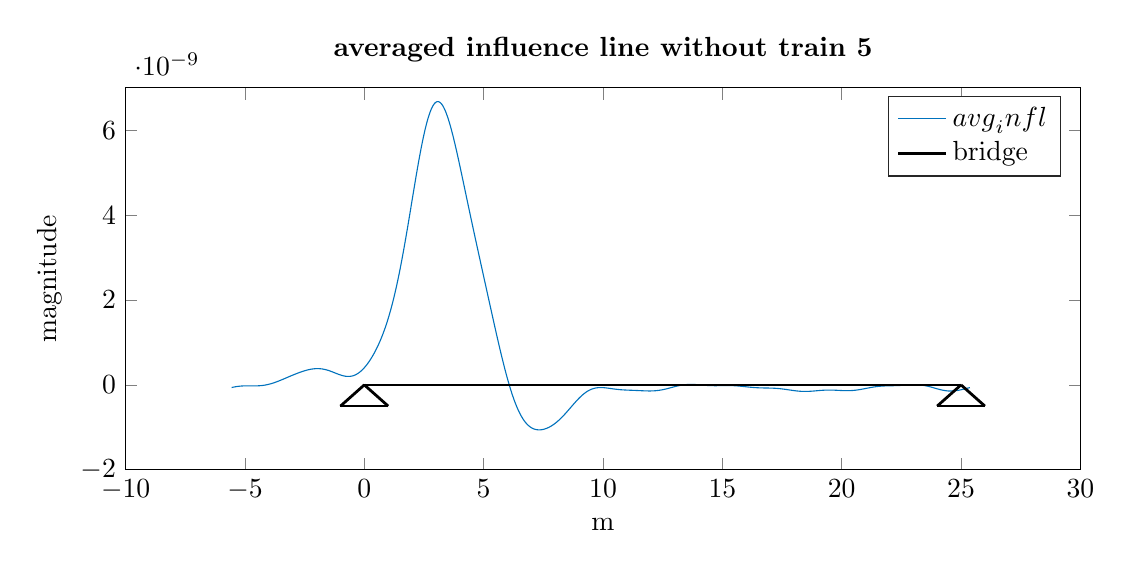
\begin{tikzpicture}

  \begin{axis}[%
    width=\textwidth,
    height=0.4\textwidth,
    at={(0\textwidth,0\textwidth)},
    scale only axis,
    xmin=-10,
    xmax=30,
    xlabel={m},
    ymin=-2e-09,
    ymax=7e-09,
    ylabel={magnitude},
    axis background/.style={fill=white},
    title style={font=\bfseries},
    title={averaged influence line without train 5},
    legend style={legend cell align=left,align=left,draw=white!15!black}
    ]
    \addplot [color=mycolor1,solid]
    table[row sep=crcr]{%
    -5.5590986328125	-6.19473989161643e-11\\
    -5.53894921875	-5.94509245073305e-11\\
    -5.5187998046875	-5.70172231016417e-11\\
    -5.498650390625	-5.4650580181018e-11\\
    -5.4785009765625	-5.23549810350598e-11\\
    -5.4583515625	-5.01340996692129e-11\\
    -5.4382021484375	-4.79912887977374e-11\\
    -5.418052734375	-4.59295709505302e-11\\
    -5.3979033203125	-4.39516307187911e-11\\
    -5.37775390625	-4.20598081603463e-11\\
    -5.3576044921875	-4.02560933812494e-11\\
    -5.337455078125	-3.85421223059915e-11\\
    -5.3173056640625	-3.69191736443782e-11\\
    -5.29715625	-3.53881670588134e-11\\
    -5.2770068359375	-3.39496625314331e-11\\
    -5.256857421875	-3.26038609262377e-11\\
    -5.2367080078125	-3.13506057371311e-11\\
    -5.21655859375	-3.01893860085751e-11\\
    -5.1964091796875	-2.91193404114199e-11\\
    -5.176259765625	-2.81392624524472e-11\\
    -5.1561103515625	-2.7247606792181e-11\\
    -5.1359609375	-2.64424966416974e-11\\
    -5.1158115234375	-2.57217322054461e-11\\
    -5.095662109375	-2.50828001335105e-11\\
    -5.0755126953125	-2.45228839433192e-11\\
    -5.05536328125	-2.40388753675564e-11\\
    -5.0352138671875	-2.36273865819459e-11\\
    -5.015064453125	-2.32847632636743e-11\\
    -4.9949150390625	-2.3007098428541e-11\\
    -4.974765625	-2.27902469924265e-11\\
    -4.9546162109375	-2.26298410003939e-11\\
    -4.934466796875	-2.25213054647167e-11\\
    -4.9143173828125	-2.2459874751278e-11\\
    -4.89416796875	-2.24406094522418e-11\\
    -4.8740185546875	-2.24584136815502e-11\\
    -4.853869140625	-2.25080527287153e-11\\
    -4.8337197265625	-2.25841710055371e-11\\
    -4.8135703125	-2.26813102198143e-11\\
    -4.7934208984375	-2.27939277097578e-11\\
    -4.773271484375	-2.2916414872774e-11\\
    -4.7531220703125	-2.30431156224444e-11\\
    -4.73297265625	-2.31683448079632e-11\\
    -4.7128232421875	-2.32864065309968e-11\\
    -4.692673828125	-2.33916122958127e-11\\
    -4.6725244140625	-2.34782989297504e-11\\
    -4.652375	-2.35408462124531e-11\\
    -4.6322255859375	-2.35736941539622e-11\\
    -4.612076171875	-2.35713598635899e-11\\
    -4.5919267578125	-2.35284539535865e-11\\
    -4.57177734375	-2.34396964238667e-11\\
    -4.5516279296875	-2.32999319765318e-11\\
    -4.531478515625	-2.31041447116023e-11\\
    -4.5113291015625	-2.28474721581459e-11\\
    -4.4911796875	-2.25252185980279e-11\\
    -4.4710302734375	-2.21328676426122e-11\\
    -4.450880859375	-2.16660940260077e-11\\
    -4.4307314453125	-2.11207745818744e-11\\
    -4.41058203125	-2.04929983742594e-11\\
    -4.3904326171875	-1.97790759565768e-11\\
    -4.370283203125	-1.89755477364652e-11\\
    -4.3501337890625	-1.80791914280249e-11\\
    -4.329984375	-1.70870285767093e-11\\
    -4.3098349609375	-1.59963301459527e-11\\
    -4.289685546875	-1.48046211584666e-11\\
    -4.2695361328125	-1.35096843889489e-11\\
    -4.24938671875	-1.21095631087934e-11\\
    -4.2292373046875	-1.06025628871621e-11\\
    -4.209087890625	-8.98725245653645e-12\\
    -4.1889384765625	-7.26246365455498e-12\\
    -4.1687890625	-5.42729045754438e-12\\
    -4.1486396484375	-3.48108712469617e-12\\
    -4.128490234375	-1.42346547523829e-12\\
    -4.1083408203125	7.45708675725067e-13\\
    -4.08819140625	3.02631989385875e-12\\
    -4.0680419921875	5.41800828287093e-12\\
    -4.047892578125	7.92017538764568e-12\\
    -4.0277431640625	1.05319908057751e-11\\
    -4.00759375	1.3252399467493e-11\\
    -3.9874443359375	1.60801295416503e-11\\
    -3.967294921875	1.90137009232312e-11\\
    -3.9471455078125	2.20514342559431e-11\\
    -3.92699609375	2.51914604416901e-11\\
    -3.9068466796875	2.8431730587188e-11\\
    -3.886697265625	3.1770026336724e-11\\
    -3.8665478515625	3.52039705389362e-11\\
    -3.8463984375	3.87310381946982e-11\\
    -3.8262490234375	4.23485676325505e-11\\
    -3.806099609375	4.60537718577815e-11\\
    -3.7859501953125	4.98437500210992e-11\\
    -3.76580078125	5.37154989529655e-11\\
    -3.7456513671875	5.76659247099859e-11\\
    -3.725501953125	6.1691854080337e-11\\
    -3.7053525390625	6.579004599601e-11\\
    -3.685203125	6.99572028006879e-11\\
    -3.6650537109375	7.41899813233162e-11\\
    -3.644904296875	7.84850037089237e-11\\
    -3.6247548828125	8.28388679598939e-11\\
    -3.60460546875	8.72481581427979e-11\\
    -3.5844560546875	9.17094542179632e-11\\
    -3.564306640625	9.62193414512088e-11\\
    -3.5441572265625	1.00774419369608e-10\\
    -3.5240078125	1.05371310225753e-10\\
    -3.5038583984375	1.10006666937702e-10\\
    -3.483708984375	1.14677180474726e-10\\
    -3.4635595703125	1.19379586661943e-10\\
    -3.44341015625	1.24110672380069e-10\\
    -3.4232607421875	1.28867281139738e-10\\
    -3.403111328125	1.33646318013163e-10\\
    -3.3829619140625	1.38444753909266e-10\\
    -3.3628125	1.43259629181866e-10\\
    -3.3426630859375	1.4808805656398e-10\\
    -3.322513671875	1.52927223424801e-10\\
    -3.3023642578125	1.57774393349411e-10\\
    -3.28221484375	1.62626907044832e-10\\
    -3.2620654296875	1.67482182579468e-10\\
    -3.241916015625	1.7233771496645e-10\\
    -3.2217666015625	1.77191075104817e-10\\
    -3.2016171875	1.8203990809578e-10\\
    -3.1814677734375	1.8688193095454e-10\\
    -3.161318359375	1.9171492974137e-10\\
    -3.1411689453125	1.96536756138595e-10\\
    -3.12101953125	2.01345323503144e-10\\
    -3.1008701171875	2.06138602427045e-10\\
    -3.080720703125	2.10914615840921e-10\\
    -3.0605712890625	2.15671433697971e-10\\
    -3.040421875	2.20407167278281e-10\\
    -3.0202724609375	2.25119963155358e-10\\
    -3.000123046875	2.29807996868752e-10\\
    -2.9799736328125	2.34469466348325e-10\\
    -2.95982421875	2.39102585137242e-10\\
    -2.9396748046875	2.43705575462047e-10\\
    -2.919525390625	2.48276661199255e-10\\
    -2.8993759765625	2.52814060788713e-10\\
    -2.8792265625	2.57315980144598e-10\\
    -2.8590771484375	2.61780605615274e-10\\
    -2.838927734375	2.66206097043336e-10\\
    -2.8187783203125	2.7059058097706e-10\\
    -2.79862890625	2.74932144084118e-10\\
    -2.7784794921875	2.79228826817766e-10\\
    -2.758330078125	2.83478617384915e-10\\
    -2.7381806640625	2.87679446064354e-10\\
    -2.71803125	2.9182917992211e-10\\
    -2.6978818359375	2.95925617969321e-10\\
    -2.677732421875	2.99966486806281e-10\\
    -2.6575830078125	3.03949436794246e-10\\
    -2.63743359375	3.07872038794426e-10\\
    -2.6172841796875	3.11731781511145e-10\\
    -2.597134765625	3.15526069473574e-10\\
    -2.5769853515625	3.1925222168759e-10\\
    -2.5568359375	3.22907470986431e-10\\
    -2.5366865234375	3.26488964105623e-10\\
    -2.516537109375	3.29993762504427e-10\\
    -2.4963876953125	3.33418843952628e-10\\
    -2.47623828125	3.36761104897977e-10\\
    -2.4560888671875	3.40017363625946e-10\\
    -2.435939453125	3.43184364219764e-10\\
    -2.4157900390625	3.46258781324891e-10\\
    -2.395640625	3.49237225718207e-10\\
    -2.3754912109375	3.52116250678359e-10\\
    -2.355341796875	3.54892359149716e-10\\
    -2.3351923828125	3.57562011688501e-10\\
    -2.31504296875	3.60121635175718e-10\\
    -2.2948935546875	3.62567632277601e-10\\
    -2.274744140625	3.64896391630461e-10\\
    -2.2545947265625	3.67104298722982e-10\\
    -2.2344453125	3.69187747445355e-10\\
    -2.2142958984375	3.71143152270914e-10\\
    -2.194146484375	3.72966961032528e-10\\
    -2.1739970703125	3.74655668252513e-10\\
    -2.15384765625	3.76205828981631e-10\\
    -2.1336982421875	3.77614073099626e-10\\
    -2.113548828125	3.78877120026803e-10\\
    -2.0933994140625	3.79991793793461e-10\\
    -2.07325	3.80955038411373e-10\\
    -2.0531005859375	3.81763933489252e-10\\
    -2.032951171875	3.82415710031961e-10\\
    -2.0128017578125	3.82907766361394e-10\\
    -1.99265234375	3.83237684095306e-10\\
    -1.9725029296875	3.83403244118977e-10\\
    -1.952353515625	3.834024424835e-10\\
    -1.9322041015625	3.83233506163618e-10\\
    -1.9120546875	3.82894908607462e-10\\
    -1.8919052734375	3.82385385010254e-10\\
    -1.871755859375	3.81703947244027e-10\\
    -1.8516064453125	3.80849898375673e-10\\
    -1.83145703125	3.79822846706253e-10\\
    -1.8113076171875	3.78622719265268e-10\\
    -1.791158203125	3.77249774694838e-10\\
    -1.7710087890625	3.75704615460078e-10\\
    -1.750859375	3.7398819932375e-10\\
    -1.7307099609375	3.72101850025208e-10\\
    -1.710560546875	3.70047267105981e-10\\
    -1.6904111328125	3.67826534826823e-10\\
    -1.67026171875	3.65442130123911e-10\\
    -1.6501123046875	3.628969295549e-10\\
    -1.629962890625	3.60194215188837e-10\\
    -1.6098134765625	3.57337679397479e-10\\
    -1.5896640625	3.543314285093e-10\\
    -1.5695146484375	3.51179985291417e-10\\
    -1.549365234375	3.47888290228827e-10\\
    -1.5292158203125	3.44461701574659e-10\\
    -1.50906640625	3.40905994149634e-10\\
    -1.4889169921875	3.37227356873548e-10\\
    -1.468767578125	3.33432389016393e-10\\
    -1.4486181640625	3.29528095161522e-10\\
    -1.42846875	3.25521878878329e-10\\
    -1.4083193359375	3.21421535106855e-10\\
    -1.388169921875	3.17235241261892e-10\\
    -1.3680205078125	3.12971547069228e-10\\
    -1.34787109375	3.08639363151869e-10\\
    -1.3277216796875	3.04247948389136e-10\\
    -1.307572265625	2.99806896076703e-10\\
    -1.2874228515625	2.95326118920657e-10\\
    -1.2672734375	2.90815832903661e-10\\
    -1.2471240234375	2.86286540066191e-10\\
    -1.226974609375	2.81749010250623e-10\\
    -1.2068251953125	2.77214261860575e-10\\
    -1.18667578125	2.72693541692441e-10\\
    -1.1665263671875	2.68198303900371e-10\\
    -1.146376953125	2.63740188160121e-10\\
    -1.1262275390625	2.59330997101119e-10\\
    -1.106078125	2.54982673079815e-10\\
    -1.0859287109375	2.50707274370872e-10\\
    -1.065779296875	2.46516950855943e-10\\
    -1.0456298828125	2.42423919292752e-10\\
    -1.02548046875	2.38440438249815e-10\\
    -1.0053310546875	2.34578782794536e-10\\
    -0.985181640624999	2.30851219024386e-10\\
    -0.965032226562499	2.27269978532649e-10\\
    -0.9448828125	2.23847232901538e-10\\
    -0.924733398437499	2.20595068316537e-10\\
    -0.904583984374999	2.175254603965e-10\\
    -0.884434570312499	2.14650249334335e-10\\
    -0.864285156249999	2.11981115443057e-10\\
    -0.8441357421875	2.0952955520158e-10\\
    -0.823986328124999	2.07306857893796e-10\\
    -0.803836914062499	2.05324082933342e-10\\
    -0.783687499999999	2.03592037964928e-10\\
    -0.763538085937499	2.02121257831123e-10\\
    -0.743388671875	2.0092198449131e-10\\
    -0.723239257812499	2.00004147976775e-10\\
    -0.703089843749999	1.99377348462972e-10\\
    -0.682940429687499	1.99050839536602e-10\\
    -0.662791015624999	1.99033512731474e-10\\
    -0.642641601562499	1.99333883403081e-10\\
    -0.622492187499999	1.9996007800747e-10\\
    -0.602342773437499	2.00919822845364e-10\\
    -0.582193359374999	2.02220434327488e-10\\
    -0.562043945312499	2.03868810811914e-10\\
    -0.541894531249999	2.05871426058659e-10\\
    -0.521745117187499	2.08234324341134e-10\\
    -0.501595703124999	2.10963117248029e-10\\
    -0.481446289062499	2.14062982203108e-10\\
    -0.461296875	2.17538662724014e-10\\
    -0.441147460937499	2.21394470434723e-10\\
    -0.420998046874999	2.25634288839631e-10\\
    -0.400848632812499	2.302615788605e-10\\
    -0.380699218749999	2.35279386130673e-10\\
    -0.3605498046875	2.40690350034038e-10\\
    -0.340400390624999	2.46496714469271e-10\\
    -0.320250976562499	2.52700340312944e-10\\
    -0.300101562499999	2.59302719548099e-10\\
    -0.279952148437499	2.66304991018e-10\\
    -0.259802734375	2.73707957757889e-10\\
    -0.239653320312499	2.8151210585083e-10\\
    -0.219503906249999	2.89717624747054e-10\\
    -0.199354492187499	2.983244289797e-10\\
    -0.179205078124999	3.07332181203532e-10\\
    -0.1590556640625	3.16740316477014e-10\\
    -0.138906249999999	3.26548067702223e-10\\
    -0.118756835937499	3.36754492131359e-10\\
    -0.0986074218749993	3.47358498843191e-10\\
    -0.0784580078124995	3.58358877087636e-10\\
    -0.0583085937499987	3.69754325391826e-10\\
    -0.0381591796874989	3.81543481316514e-10\\
    -0.0180097656249991	3.93724951747536e-10\\
    0.0021396484375007	4.06297343603243e-10\\
    0.0222890625000005	4.19259294835447e-10\\
    0.0424384765625012	4.32609505598434e-10\\
    0.062587890625001	4.46346769458011e-10\\
    0.0827373046875008	4.60470004510477e-10\\
    0.102886718750001	4.74978284279681e-10\\
    0.1230361328125	4.8987086825912e-10\\
    0.143185546875001	5.05147231965316e-10\\
    0.163334960937501	5.20807096368371e-10\\
    0.183484375000001	5.36850456565885e-10\\
    0.203633789062501	5.5327760956706e-10\\
    0.223783203125	5.70089181055027e-10\\
    0.243932617187501	5.87286150997151e-10\\
    0.264082031250001	6.04869877975151e-10\\
    0.284231445312501	6.22842122109677e-10\\
    0.304380859375001	6.41205066456998e-10\\
    0.3245302734375	6.59961336759184e-10\\
    0.344679687500001	6.79114019433252e-10\\
    0.364829101562501	6.98666677689293e-10\\
    0.384978515625001	7.18623365672643e-10\\
    0.405127929687501	7.38988640530625e-10\\
    0.42527734375	7.5976757231029e-10\\
    0.445426757812501	7.80965751599858e-10\\
    0.465576171875001	8.02589294833291e-10\\
    0.485725585937501	8.24644847184475e-10\\
    0.505875000000001	8.47139582984919e-10\\
    0.526024414062501	8.70081203606635e-10\\
    0.546173828125001	8.93477932759917e-10\\
    0.566323242187501	9.17338509164079e-10\\
    0.586472656250001	9.4167217655783e-10\\
    0.6066220703125	9.66488671024768e-10\\
    0.626771484375001	9.91798205618535e-10\\
    0.646920898437501	1.01761145228135e-09\\
    0.667070312500001	1.04393952105902e-09\\
    0.687219726562501	1.07079393662498e-09\\
    0.707369140625	1.09818661213539e-09\\
    0.727518554687501	1.12612982044706e-09\\
    0.747667968750001	1.15463616273939e-09\\
    0.767817382812501	1.18371853459127e-09\\
    0.787966796875001	1.21339008957331e-09\\
    0.8081162109375	1.2436642004253e-09\\
    0.828265625000001	1.27455441789809e-09\\
    0.848415039062501	1.30607442734842e-09\\
    0.868564453125001	1.33823800318391e-09\\
    0.888713867187501	1.3710589612647e-09\\
    0.90886328125	1.40455110937636e-09\\
    0.929012695312501	1.43872819589724e-09\\
    0.949162109375001	1.47360385679125e-09\\
    0.969311523437501	1.50919156106475e-09\\
    0.989460937500001	1.54550455483363e-09\\
    1.0096103515625	1.58255580415327e-09\\
    1.029759765625	1.62035793677068e-09\\
    1.0499091796875	1.65892318296425e-09\\
    1.07005859375	1.6982633156418e-09\\
    1.0902080078125	1.73838958987288e-09\\
    1.110357421875	1.77931268203574e-09\\
    1.1305068359375	1.82104262876329e-09\\
    1.15065625	1.86358876587598e-09\\
    1.1708056640625	1.90695966749229e-09\\
    1.190955078125	1.95116308550971e-09\\
    1.2111044921875	1.99620588965106e-09\\
    1.23125390625	2.04209400827171e-09\\
    1.2514033203125	2.08883237012408e-09\\
    1.271552734375	2.13642484727528e-09\\
    1.2917021484375	2.18487419937331e-09\\
    1.3118515625	2.23418201945536e-09\\
    1.3320009765625	2.28434868149029e-09\\
    1.352150390625	2.33537328984399e-09\\
    1.3722998046875	2.38725363085353e-09\\
    1.39244921875	2.43998612669176e-09\\
    1.4125986328125	2.49356579169951e-09\\
    1.432748046875	2.54798619135753e-09\\
    1.4528974609375	2.60323940406415e-09\\
    1.473046875	2.65931598587876e-09\\
    1.4931962890625	2.71620493838387e-09\\
    1.513345703125	2.77389367981133e-09\\
    1.5334951171875	2.83236801957011e-09\\
    1.55364453125	2.89161213630463e-09\\
    1.5737939453125	2.95160855960362e-09\\
    1.593943359375	3.01233815546995e-09\\
    1.6140927734375	3.07378011565222e-09\\
    1.6342421875	3.13591195092831e-09\\
    1.6543916015625	3.19870948842063e-09\\
    1.674541015625	3.26214687301186e-09\\
    1.6946904296875	3.32619657291839e-09\\
    1.71483984375	3.39082938946738e-09\\
    1.7349892578125	3.45601447111146e-09\\
    1.755138671875	3.52171933170274e-09\\
    1.7752880859375	3.58790987303624e-09\\
    1.7954375	3.65455041165976e-09\\
    1.8155869140625	3.72160370993551e-09\\
    1.835736328125	3.78903101132569e-09\\
    1.8558857421875	3.85679207986226e-09\\
    1.87603515625	3.92484524374821e-09\\
    1.8961845703125	3.99314744302566e-09\\
    1.916333984375	4.06165428123346e-09\\
    1.9364833984375	4.13032008096494e-09\\
    1.9566328125	4.19909794322459e-09\\
    1.9767822265625	4.26793981047044e-09\\
    1.996931640625	4.33679653321771e-09\\
    2.0170810546875	4.40561794006766e-09\\
    2.03723046875	4.47435291101534e-09\\
    2.0573798828125	4.54294945387871e-09\\
    2.077529296875	4.611354783682e-09\\
    2.0976787109375	4.67951540481643e-09\\
    2.117828125	4.74737719579194e-09\\
    2.1379775390625	4.8148854963853e-09\\
    2.158126953125	4.88198519698143e-09\\
    2.1782763671875	4.94862082989738e-09\\
    2.19842578125	5.01473666247133e-09\\
    2.2185751953125	5.08027679169258e-09\\
    2.238724609375	5.14518524014252e-09\\
    2.2588740234375	5.20940605301193e-09\\
    2.2790234375	5.27288339595483e-09\\
    2.2991728515625	5.33556165353591e-09\\
    2.319322265625	5.39738552802522e-09\\
    2.3394716796875	5.45830013829144e-09\\
    2.35962109375	5.51825111854357e-09\\
    2.3797705078125	5.57718471666984e-09\\
    2.399919921875	5.63504789192257e-09\\
    2.4200693359375	5.69178841169825e-09\\
    2.44021875	5.74735494716348e-09\\
    2.4603681640625	5.8016971674795e-09\\
    2.480517578125	5.85476583238075e-09\\
    2.5006669921875	5.90651288286646e-09\\
    2.52081640625	5.95689152976883e-09\\
    2.5409658203125	6.00585633996565e-09\\
    2.561115234375	6.05336332001184e-09\\
    2.5812646484375	6.09936999696972e-09\\
    2.6014140625	6.14383549622577e-09\\
    2.6215634765625	6.18672061608861e-09\\
    2.641712890625	6.22798789897164e-09\\
    2.6618623046875	6.26760169897252e-09\\
    2.68201171875	6.30552824567117e-09\\
    2.7021611328125	6.34173570397788e-09\\
    2.722310546875	6.37619422987391e-09\\
    2.7424599609375	6.40887602189775e-09\\
    2.762609375	6.4397553682416e-09\\
    2.7827587890625	6.46880868933499e-09\\
    2.802908203125	6.49601457580407e-09\\
    2.8230576171875	6.52135382170832e-09\\
    2.84320703125	6.54480945296895e-09\\
    2.8633564453125	6.56636675091668e-09\\
    2.883505859375	6.58601327089986e-09\\
    2.9036552734375	6.60373885590767e-09\\
    2.9238046875	6.61953564517673e-09\\
    2.9439541015625	6.63339807776344e-09\\
    2.964103515625	6.64532289107819e-09\\
    2.9842529296875	6.65530911439152e-09\\
    3.00440234375	6.66335805733652e-09\\
    3.0245517578125	6.66947329344493e-09\\
    3.044701171875	6.67366063876907e-09\\
    3.0648505859375	6.67592812565439e-09\\
    3.085	6.67628597174155e-09\\
    3.1051494140625	6.67474654428972e-09\\
    3.125298828125	6.67132431992563e-09\\
    3.1454482421875	6.66603583993593e-09\\
    3.16559765625	6.65889966123193e-09\\
    3.1857470703125	6.64993630312833e-09\\
    3.205896484375	6.63916819008845e-09\\
    3.2260458984375	6.6266195905996e-09\\
    3.2461953125	6.61231655235274e-09\\
    3.2663447265625	6.59628683391036e-09\\
    3.286494140625	6.57855983305586e-09\\
    3.3066435546875	6.55916651202676e-09\\
    3.32679296875	6.53813931984171e-09\\
    3.3469423828125	6.51551211193939e-09\\
    3.367091796875	6.49132006735376e-09\\
    3.3872412109375	6.46559960365668e-09\\
    3.407390625	6.43838828990406e-09\\
    3.4275400390625	6.40972475782675e-09\\
    3.447689453125	6.37964861151131e-09\\
    3.4678388671875	6.3482003358191e-09\\
    3.48798828125	6.31542120379462e-09\\
    3.5081376953125	6.281353183316e-09\\
    3.528287109375	6.2460388432415e-09\\
    3.5484365234375	6.20952125930591e-09\\
    3.5685859375	6.17184392002079e-09\\
    3.5887353515625	6.13305063283073e-09\\
    3.608884765625	6.09318543077602e-09\\
    3.6290341796875	6.05229247990952e-09\\
    3.64918359375	6.01041598771178e-09\\
    3.6693330078125	5.96760011274436e-09\\
    3.689482421875	5.9238888757766e-09\\
    3.7096318359375	5.87932607261509e-09\\
    3.72978125	5.83395518885924e-09\\
    3.7499306640625	5.7878193167991e-09\\
    3.770080078125	5.74096107466426e-09\\
    3.7902294921875	5.69342252842446e-09\\
    3.81037890625	5.64524511633365e-09\\
    3.8305283203125	5.59646957640037e-09\\
    3.850677734375	5.54713587695699e-09\\
    3.8708271484375	5.49728315049073e-09\\
    3.8909765625	5.44694963088803e-09\\
    3.9111259765625	5.39617259423327e-09\\
    3.931275390625	5.3449883032909e-09\\
    3.9514248046875	5.2934319557886e-09\\
    3.97157421875	5.24153763660657e-09\\
    3.9917236328125	5.18933827396595e-09\\
    4.011873046875	5.13686559969658e-09\\
    4.0320224609375	5.08415011365152e-09\\
    4.052171875	5.03122105232298e-09\\
    4.0723212890625	4.9781063617009e-09\\
    4.092470703125	4.9248326744028e-09\\
    4.1126201171875	4.87142529108991e-09\\
    4.13276953125	4.81790816617199e-09\\
    4.1529189453125	4.76430389778975e-09\\
    4.173068359375	4.71063372205129e-09\\
    4.1932177734375	4.6569175114859e-09\\
    4.2133671875	4.60317377766623e-09\\
    4.2335166015625	4.54941967793726e-09\\
    4.253666015625	4.49567102617874e-09\\
    4.2738154296875	4.44194230751549e-09\\
    4.29396484375	4.38824669687924e-09\\
    4.3141142578125	4.33459608131389e-09\\
    4.334263671875	4.28100108590591e-09\\
    4.3544130859375	4.22747110321123e-09\\
    4.3745625	4.17401432604024e-09\\
    4.3947119140625	4.12063778345332e-09\\
    4.414861328125	4.0673473798105e-09\\
    4.4350107421875	4.01414793671092e-09\\
    4.45516015625	3.96104323764999e-09\\
    4.4753095703125	3.90803607521517e-09\\
    4.495458984375	3.85512830063511e-09\\
    4.5156083984375	3.80232087549102e-09\\
    4.5357578125	3.74961392539401e-09\\
    4.5559072265625	3.69700679542794e-09\\
    4.576056640625	3.6444981071534e-09\\
    4.5962060546875	3.59208581696538e-09\\
    4.61635546875	3.53976727559505e-09\\
    4.6365048828125	3.48753928854403e-09\\
    4.656654296875	3.43539817723891e-09\\
    4.6768037109375	3.38333984069322e-09\\
    4.696953125	3.33135981746467e-09\\
    4.7171025390625	3.27945334769631e-09\\
    4.737251953125	3.22761543503234e-09\\
    4.7574013671875	3.17584090820145e-09\\
    4.77755078125	3.12412448206375e-09\\
    4.7977001953125	3.07246081792125e-09\\
    4.817849609375	3.02084458289589e-09\\
    4.8379990234375	2.96927050818426e-09\\
    4.8581484375	2.91773344600378e-09\\
    4.8782978515625	2.86622842505106e-09\\
    4.898447265625	2.81475070429983e-09\\
    4.9185966796875	2.76329582497308e-09\\
    4.93874609375	2.71185966053178e-09\\
    4.9588955078125	2.66043846453035e-09\\
    4.979044921875	2.60902891619802e-09\\
    4.9991943359375	2.55762816361385e-09\\
    5.01934375	2.50623386435269e-09\\
    5.0394931640625	2.45484422348886e-09\\
    5.059642578125	2.40345802885446e-09\\
    5.0797919921875	2.35207468345926e-09\\
    5.09994140625	2.30069423498967e-09\\
    5.1200908203125	2.24931740231492e-09\\
    5.140240234375	2.19794559893937e-09\\
    5.1603896484375	2.1465809533507e-09\\
    5.1805390625	2.09522632622483e-09\\
    5.2006884765625	2.04388532445948e-09\\
    5.220837890625	1.99256231201908e-09\\
    5.2409873046875	1.94126241758516e-09\\
    5.26113671875	1.88999153901681e-09\\
    5.2812861328125	1.83875634463707e-09\\
    5.301435546875	1.78756427137153e-09\\
    5.3215849609375	1.73642351977598e-09\\
    5.341734375	1.68534304600044e-09\\
    5.3618837890625	1.63433255074666e-09\\
    5.382033203125	1.58340246528623e-09\\
    5.4021826171875	1.53256393461586e-09\\
    5.42233203125	1.48182879783533e-09\\
    5.4424814453125	1.4312095658427e-09\\
    5.462630859375	1.3807193964496e-09\\
    5.4827802734375	1.3303720670272e-09\\
    5.5029296875	1.28018194480136e-09\\
    5.5230791015625	1.23016395492217e-09\\
    5.543228515625	1.18033354643985e-09\\
    5.5633779296875	1.13070665632491e-09\\
    5.58352734375	1.08129967167602e-09\\
    5.6036767578125	1.03212939026422e-09\\
    5.623826171875	9.8321297956618e-10\\
    5.6439755859375	9.34567934443383e-10\\
    5.664125	8.86212033627339e-10\\
    5.6842744140625	8.38163295173549e-10\\
    5.704423828125	7.90439931049191e-10\\
    5.7245732421875	7.43060301020986e-10\\
    5.74472265625	6.96042866010662e-10\\
    5.7648720703125	6.49406141085794e-10\\
    5.785021484375	6.03168648253583e-10\\
    5.8051708984375	5.57348869224325e-10\\
    5.8253203125	5.11965198309932e-10\\
    5.8454697265625	4.67035895620943e-10\\
    5.865619140625	4.22579040722938e-10\\
    5.8857685546875	3.7861248691024e-10\\
    5.90591796875	3.35153816251219e-10\\
    5.9260673828125	2.92220295555418e-10\\
    5.946216796875	2.49828833408169e-10\\
    5.9663662109375	2.07995938413292e-10\\
    5.986515625	1.66737678779006e-10\\
    6.0066650390625	1.26069643376193e-10\\
    6.026814453125	8.60069043919025e-11\\
    6.0469638671875	4.65639816941732e-11\\
    6.06711328125	7.75480901727016e-12\\
    6.0872626953125	-3.04072979310397e-11\\
    6.107412109375	-6.79096713461865e-11\\
    6.1275615234375	-1.0474031910149e-10\\
    6.1477109375	-1.40887950343036e-10\\
    6.1678603515625	-1.76341998835361e-10\\
    6.188009765625	-2.11092643997139e-10\\
    6.2081591796875	-2.45130829574806e-10\\
    6.22830859375	-2.78448279910896e-10\\
    6.2484580078125	-3.11037513772797e-10\\
    6.268607421875	-3.42891855716591e-10\\
    6.2887568359375	-3.74005444969645e-10\\
    6.30890625	-4.04373241824594e-10\\
    6.3290556640625	-4.33991031546263e-10\\
    6.349205078125	-4.62855425801938e-10\\
    6.3693544921875	-4.90963861634129e-10\\
    6.38950390625	-5.18314598003532e-10\\
    6.4096533203125	-5.44906709938372e-10\\
    6.429802734375	-5.70740080334463e-10\\
    6.4499521484375	-5.95815389458379e-10\\
    6.4701015625	-6.20134102213819e-10\\
    6.4902509765625	-6.43698453238731e-10\\
    6.510400390625	-6.66511429907914e-10\\
    6.5305498046875	-6.88576753322618e-10\\
    6.55069921875	-7.09898857375151e-10\\
    6.5708486328125	-7.30482865982596e-10\\
    6.590998046875	-7.50334568589438e-10\\
    6.6111474609375	-7.69460394044219e-10\\
    6.631296875	-7.87867382960177e-10\\
    6.6514462890625	-8.05563158674286e-10\\
    6.671595703125	-8.2255589692308e-10\\
    6.6917451171875	-8.38854294357154e-10\\
    6.71189453125	-8.54467536019269e-10\\
    6.7320439453125	-8.69405261913568e-10\\
    6.752193359375	-8.83677532795455e-10\\
    6.7723427734375	-8.97294795313271e-10\\
    6.7924921875	-9.10267846634014e-10\\
    6.8126416015625	-9.22607798685894e-10\\
    6.832791015625	-9.34326042150652e-10\\
    6.8529404296875	-9.45434210338163e-10\\
    6.87308984375	-9.55944143074963e-10\\
    6.8932392578125	-9.65867850736994e-10\\
    6.913388671875	-9.75217478555031e-10\\
    6.9335380859375	-9.84005271318969e-10\\
    6.9536875	-9.92243538604424e-10\\
    6.9738369140625	-9.99944620641917e-10\\
    6.993986328125	-1.00712085494534e-09\\
    7.0141357421875	-1.0137845438124e-09\\
    7.03428515625	-1.01994792280535e-09\\
    7.0544345703125	-1.02562313031554e-09\\
    7.074583984375	-1.03082217831041e-09\\
    7.0947333984375	-1.03555692435574e-09\\
    7.1148828125	-1.03983904500066e-09\\
    7.1350322265625	-1.04368001060669e-09\\
    7.155181640625	-1.04709106169578e-09\\
    7.1753310546875	-1.05008318688605e-09\\
    7.19548046875	-1.05266710247685e-09\\
    7.2156298828125	-1.05485323373838e-09\\
    7.235779296875	-1.0566516979535e-09\\
    7.2559287109375	-1.05807228925268e-09\\
    7.276078125	-1.05912446527554e-09\\
    7.2962275390625	-1.05981733568501e-09\\
    7.316376953125	-1.06015965255309e-09\\
    7.3365263671875	-1.06015980262941e-09\\
    7.35667578125	-1.05982580149665e-09\\
    7.3768251953125	-1.0591652896095e-09\\
    7.396974609375	-1.05818553020649e-09\\
    7.4171240234375	-1.05689340907688e-09\\
    7.4372734375	-1.05529543615779e-09\\
    7.4574228515625	-1.05339774892968e-09\\
    7.477572265625	-1.05120611757178e-09\\
    7.4977216796875	-1.04872595183215e-09\\
    7.51787109375	-1.04596230956123e-09\\
    7.5380205078125	-1.04291990685112e-09\\
    7.558169921875	-1.03960312971728e-09\\
    7.5783193359375	-1.03601604725379e-09\\
    7.59846875	-1.03216242618801e-09\\
    7.6186181640625	-1.02804574675539e-09\\
    7.638767578125	-1.02366921981093e-09\\
    7.6589169921875	-1.01903580508924e-09\\
    7.67906640625	-1.01414823052134e-09\\
    7.6992158203125	-1.00900901251299e-09\\
    7.719365234375	-1.00362047708593e-09\\
    7.7395146484375	-9.97984781781092e-10\\
    7.7596640625	-9.92103938220074e-10\\
    7.7798134765625	-9.8597983521965e-10\\
    7.799962890625	-9.79614262352401e-10\\
    7.8201123046875	-9.73008933845535e-10\\
    7.84026171875	-9.66165512709347e-10\\
    7.8604111328125	-9.5908563498651e-10\\
    7.880560546875	-9.51770934013624e-10\\
    7.9007099609375	-9.4422306458704e-10\\
    7.920859375	-9.36443726926022e-10\\
    7.9410087890625	-9.28434690327734e-10\\
    7.961158203125	-9.20197816410393e-10\\
    7.9813076171875	-9.11735081843125e-10\\
    8.00145703125	-9.03048600463689e-10\\
    8.0216064453125	-8.94140644688206e-10\\
    8.041755859375	-8.85013666120326e-10\\
    8.0619052734375	-8.75670315270971e-10\\
    8.0820546875	-8.66113460303749e-10\\
    8.1022041015625	-8.5634620472545e-10\\
    8.122353515625	-8.46371903945611e-10\\
    8.1425029296875	-8.36194180634001e-10\\
    8.16265234375	-8.25816938809971e-10\\
    8.1828017578125	-8.15244376602972e-10\\
    8.202951171875	-8.04480997629069e-10\\
    8.2231005859375	-7.93531620934025e-10\\
    8.24325	-7.82401389459425e-10\\
    8.2633994140625	-7.71095776994348e-10\\
    8.283548828125	-7.59620593581236e-10\\
    8.3036982421875	-7.4798198935089e-10\\
    8.32384765625	-7.36186456767798e-10\\
    8.3439970703125	-7.24240831273412e-10\\
    8.364146484375	-7.12152290321323e-10\\
    8.3842958984375	-6.99928350804718e-10\\
    8.4044453125	-6.87576864882791e-10\\
    8.4245947265625	-6.75106014219154e-10\\
    8.444744140625	-6.62524302651452e-10\\
    8.4648935546875	-6.49840547317557e-10\\
    8.48504296875	-6.37063868269687e-10\\
    8.5051923828125	-6.24203676613706e-10\\
    8.525341796875	-6.11269661216483e-10\\
    8.5454912109375	-5.98271774029776e-10\\
    8.565640625	-5.85220214084346e-10\\
    8.5857900390625	-5.72125410213131e-10\\
    8.605939453125	-5.58998002567102e-10\\
    8.6260888671875	-5.4584882299204e-10\\
    8.64623828125	-5.32688874338715e-10\\
    8.6663876953125	-5.19529308783019e-10\\
    8.686537109375	-5.06381405236229e-10\\
    8.7066865234375	-4.93256545929002e-10\\
    8.7268359375	-4.80166192255746e-10\\
    8.7469853515625	-4.67121859968708e-10\\
    8.767134765625	-4.54135093813458e-10\\
    8.7872841796875	-4.41217441699511e-10\\
    8.80743359375	-4.28380428501386e-10\\
    8.8275830078125	-4.15635529586748e-10\\
    8.847732421875	-4.02994144169113e-10\\
    8.8678818359375	-3.90467568583175e-10\\
    8.88803125	-3.78066969580933e-10\\
    8.9081806640625	-3.65803357746599e-10\\
    8.928330078125	-3.53687561127655e-10\\
    8.9484794921875	-3.41730199178506e-10\\
    8.96862890625	-3.29941657111827e-10\\
    8.9887783203125	-3.18332060751054e-10\\
    9.008927734375	-3.06911251975433e-10\\
    9.0290771484375	-2.95688764846717e-10\\
    9.0492265625	-2.84673802503869e-10\\
    9.0693759765625	-2.73875214909174e-10\\
    9.089525390625	-2.63301477525852e-10\\
    9.1096748046875	-2.52960671003639e-10\\
    9.12982421875	-2.42860461944986e-10\\
    9.1499736328125	-2.33008084820345e-10\\
    9.170123046875	-2.23410325096703e-10\\
    9.1902724609375	-2.14073503638856e-10\\
    9.210421875	-2.05003462438176e-10\\
    9.2305712890625	-1.96205551718611e-10\\
    9.250720703125	-1.87684618464465e-10\\
    9.2708701171875	-1.7944499640927e-10\\
    9.29101953125	-1.71490497519552e-10\\
    9.3111689453125	-1.63824405001786e-10\\
    9.331318359375	-1.56449467855217e-10\\
    9.3514677734375	-1.493678969875e-10\\
    9.3716171875	-1.42581362904402e-10\\
    9.3917666015625	-1.36090994979042e-10\\
    9.411916015625	-1.29897382300401e-10\\
    9.4320654296875	-1.24000576095071e-10\\
    9.45221484375	-1.18400093710586e-10\\
    9.4723642578125	-1.13094924142992e-10\\
    9.492513671875	-1.08083535085805e-10\\
    9.5126630859375	-1.03363881472103e-10\\
    9.5328125	-9.89334154761392e-11\\
    9.5529619140625	-9.47890979357636e-11\\
    9.573111328125	-9.09274111519221e-11\\
    9.5932607421875	-8.73443730166943e-11\\
    9.61341015625	-8.40355524167467e-11\\
    9.6335595703125	-8.09960858546589e-11\\
    9.653708984375	-7.82206952264508e-11\\
    9.6738583984375	-7.57037066897156e-11\\
    9.6940078125	-7.34390705531143e-11\\
    9.7141572265625	-7.14203821146277e-11\\
    9.734306640625	-6.96409033728496e-11\\
    9.7544560546875	-6.80935855328294e-11\\
    9.77460546875	-6.67710922254828e-11\\
    9.7947548828125	-6.56658233573969e-11\\
    9.814904296875	-6.47699395060149e-11\\
    9.8350537109375	-6.40753867736538e-11\\
    9.855203125	-6.35739220125973e-11\\
    9.8753525390625	-6.32571383326379e-11\\
    9.895501953125	-6.31164908019243e-11\\
    9.9156513671875	-6.3143322251743e-11\\
    9.93580078125	-6.33288890960245e-11\\
    9.9559501953125	-6.36643870768123e-11\\
    9.976099609375	-6.41409768477338e-11\\
    9.9962490234375	-6.47498093086373e-11\\
    10.0163984375	-6.54820506059979e-11\\
    10.0365478515625	-6.63289067154301e-11\\
    10.056697265625	-6.72816475247277e-11\\
    10.0768466796875	-6.83316303381694e-11\\
    10.09699609375	-6.94703227254902e-11\\
    10.1171455078125	-7.06893246418033e-11\\
    10.137294921875	-7.19803897479426e-11\\
    10.1574443359375	-7.33354458640918e-11\\
    10.17759375	-7.47466144932358e-11\\
    10.1977431640625	-7.62062293548262e-11\\
    10.217892578125	-7.77068538731162e-11\\
    10.2380419921875	-7.92412975688928e-11\\
    10.25819140625	-8.08026313077532e-11\\
    10.2783408203125	-8.23842013626472e-11\\
    10.298490234375	-8.39796422531199e-11\\
    10.3186396484375	-8.55828883285312e-11\\
    10.3387890625	-8.71881840674284e-11\\
    10.3589384765625	-8.87900930702648e-11\\
    10.379087890625	-9.03835057277187e-11\\
    10.3992373046875	-9.19636455519485e-11\\
    10.41938671875	-9.3526074163257e-11\\
    10.4395361328125	-9.50666949297235e-11\\
    10.459685546875	-9.65817552624968e-11\\
    10.4798349609375	-9.80678475744508e-11\\
    10.499984375	-9.95219089149402e-11\\
    10.5201337890625	-1.00941219298285e-10\\
    10.540283203125	-1.02323398748452e-10\\
    10.5604326171875	-1.03666403087093e-10\\
    10.58058203125	-1.04968518496691e-10\\
    10.6007314453125	-1.06228354894986e-10\\
    10.620880859375	-1.07444838161116e-10\\
    10.6410302734375	-1.08617201257993e-10\\
    10.6611796875	-1.09744974299315e-10\\
    10.6813291015625	-1.10827973613317e-10\\
    10.701478515625	-1.11866289858788e-10\\
    10.7216279296875	-1.12860275252132e-10\\
    10.74177734375	-1.13810529967207e-10\\
    10.7619267578125	-1.14717887772425e-10\\
    10.782076171875	-1.15583400972014e-10\\
    10.8022255859375	-1.16408324720571e-10\\
    10.822375	-1.17194100781895e-10\\
    10.8425244140625	-1.17942340804738e-10\\
    10.862673828125	-1.18654809189423e-10\\
    10.8828232421875	-1.19333405620309e-10\\
    10.90297265625	-1.19980147339823e-10\\
    10.9231220703125	-1.20597151240199e-10\\
    10.943271484375	-1.2118661584922e-10\\
    10.9634208984375	-1.21750803286084e-10\\
    10.9835703125	-1.22292021263036e-10\\
    11.0037197265625	-1.22812605207711e-10\\
    11.023869140625	-1.23314900580023e-10\\
    11.0440185546875	-1.23801245456157e-10\\
    11.06416796875	-1.24273953450615e-10\\
    11.0843173828125	-1.24735297045363e-10\\
    11.104466796875	-1.25187491393042e-10\\
    11.1246162109375	-1.25632678658782e-10\\
    11.144765625	-1.2607291296255e-10\\
    11.1649150390625	-1.26510145981125e-10\\
    11.185064453125	-1.26946213265667e-10\\
    11.2052138671875	-1.27382821327654e-10\\
    11.22536328125	-1.278215355424e-10\\
    11.2455126953125	-1.28263768915808e-10\\
    11.265662109375	-1.2871077175614e-10\\
    11.2858115234375	-1.29163622288668e-10\\
    11.3059609375	-1.29623218246992e-10\\
    11.3261103515625	-1.30090269470589e-10\\
    11.346259765625	-1.30565291533888e-10\\
    11.3664091796875	-1.31048600427794e-10\\
    11.38655859375	-1.31540308310123e-10\\
    11.4067080078125	-1.32040320336976e-10\\
    11.426857421875	-1.32548332582547e-10\\
    11.4470068359375	-1.3306383105033e-10\\
    11.46715625	-1.33586091774253e-10\\
    11.4873056640625	-1.34114182003694e-10\\
    11.507455078125	-1.34646962461989e-10\\
    11.5276044921875	-1.35183090663611e-10\\
    11.54775390625	-1.35721025270925e-10\\
    11.5679033203125	-1.36259031467234e-10\\
    11.588052734375	-1.36795187318709e-10\\
    11.6082021484375	-1.37327391093879e-10\\
    11.6283515625	-1.37853369505488e-10\\
    11.6485009765625	-1.38370686835896e-10\\
    11.668650390625	-1.38876754903683e-10\\
    11.6887998046875	-1.39368843825813e-10\\
    11.70894921875	-1.39844093526598e-10\\
    11.7290986328125	-1.40299525941779e-10\\
    11.749248046875	-1.40732057863354e-10\\
    11.7693974609375	-1.41138514368328e-10\\
    11.789546875	-1.41515642772306e-10\\
    11.8096962890625	-1.4186012704688e-10\\
    11.829845703125	-1.42168602638024e-10\\
    11.8499951171875	-1.42437671621233e-10\\
    11.87014453125	-1.42663918127902e-10\\
    11.8902939453125	-1.42843923976553e-10\\
    11.910443359375	-1.42974284441742e-10\\
    11.9305927734375	-1.43051624093167e-10\\
    11.9507421875	-1.43072612637275e-10\\
    11.9708916015625	-1.43033980693854e-10\\
    11.991041015625	-1.42932535440465e-10\\
    12.0111904296875	-1.42765176058241e-10\\
    12.03133984375	-1.42528908913527e-10\\
    12.0514892578125	-1.42220862411006e-10\\
    12.071638671875	-1.41838301455404e-10\\
    12.0917880859375	-1.41378641460576e-10\\
    12.1119375	-1.40839461846669e-10\\
    12.1320869140625	-1.40218518968262e-10\\
    12.152236328125	-1.39513758418733e-10\\
    12.1723857421875	-1.38723326658724e-10\\
    12.19253515625	-1.37845581919349e-10\\
    12.2126845703125	-1.3687910433381e-10\\
    12.232833984375	-1.35822705254209e-10\\
    12.2529833984375	-1.34675435713716e-10\\
    12.2731328125	-1.33436593997696e-10\\
    12.2932822265625	-1.32105732291052e-10\\
    12.313431640625	-1.30682662372741e-10\\
    12.3335810546875	-1.29167460332298e-10\\
    12.35373046875	-1.27560470287133e-10\\
    12.3738798828125	-1.25862307083355e-10\\
    12.394029296875	-1.24073857967007e-10\\
    12.4141787109375	-1.22196283216647e-10\\
    12.434328125	-1.20231015732403e-10\\
    12.4544775390625	-1.18179759580779e-10\\
    12.474626953125	-1.16044487498615e-10\\
    12.4947763671875	-1.13827437363768e-10\\
    12.51492578125	-1.11531107644146e-10\\
    12.5350751953125	-1.09158251840781e-10\\
    12.555224609375	-1.067118719446e-10\\
    12.5753740234375	-1.04195210930409e-10\\
    12.5955234375	-1.01611744315431e-10\\
    12.6156728515625	-9.89651708133751e-11\\
    12.635822265625	-9.6259402118564e-11\\
    12.6559716796875	-9.34985518580676e-11\\
    12.67612109375	-9.06869237529929e-11\\
    12.6962705078125	-8.78289990332044e-11\\
    12.716419921875	-8.49294231526011e-11\\
    12.7365693359375	-8.19929918548211e-11\\
    12.75671875	-7.90246366417283e-11\\
    12.7768681640625	-7.60294096993425e-11\\
    12.797017578125	-7.30124683379439e-11\\
    12.8171669921875	-6.99790590049639e-11\\
    12.83731640625	-6.69345009308419e-11\\
    12.8574658203125	-6.38841694694769e-11\\
    12.877615234375	-6.08334791959783e-11\\
    12.8977646484375	-5.77878668253645e-11\\
    12.9179140625	-5.47527740164584e-11\\
    12.9380634765625	-5.17336301256512e-11\\
    12.958212890625	-4.87358349753211e-11\\
    12.9783623046875	-4.57647417015837e-11\\
    12.99851171875	-4.28256397456924e-11\\
    13.0186611328125	-3.99237380527757e-11\\
    13.038810546875	-3.70641485407358e-11\\
    13.0589599609375	-3.4251869901041e-11\\
    13.079109375	-3.14917717917712e-11\\
    13.0992587890625	-2.87885794817217e-11\\
    13.119408203125	-2.6146859002555e-11\\
    13.1395576171875	-2.35710028639713e-11\\
    13.15970703125	-2.10652163846324e-11\\
    13.1798564453125	-1.86335046891508e-11\\
    13.200005859375	-1.62796604188191e-11\\
    13.2201552734375	-1.40072522009674e-11\\
    13.2403046875	-1.18196139188536e-11\\
    13.2604541015625	-9.71983482086573e-12\\
    13.280603515625	-7.71075050454178e-12\\
    13.3007529296875	-5.79493480752272e-12\\
    13.32090234375	-3.97469263400971e-12\\
    13.3410517578125	-2.25205374168936e-12\\
    13.361201171875	-6.2876751037674e-13\\
    13.3813505859375	8.93701290168137e-13\\
    13.4015	2.31417571964195e-12\\
    13.4216494140625	3.63176886409243e-12\\
    13.441798828125	4.8458850045089e-12\\
    13.4619482421875	5.95621975524942e-12\\
    13.48209765625	6.96275917436032e-12\\
    13.5022470703125	7.86577785178601e-12\\
    13.522396484375	8.66583598533302e-12\\
    13.5425458984375	9.36377545807586e-12\\
    13.5626953125	9.96071493471734e-12\\
    13.5828447265625	1.0458043998041e-11\\
    13.602994140625	1.08574163502722e-11\\
    13.6231435546875	1.11607421076053e-11\\
    13.64329296875	1.13701792195909e-11\\
    13.6634423828125	1.14881240482882e-11\\
    13.683591796875	1.15172011452228e-11\\
    13.7037412109375	1.1460252267135e-11\\
    13.723890625	1.13203246742961e-11\\
    13.7440400390625	1.11006587577779e-11\\
    13.764189453125	1.08046750444905e-11\\
    13.7843388671875	1.04359606310202e-11\\
    13.80448828125	9.99825509935637e-12\\
    13.8246376953125	9.49543596936533e-12\\
    13.844787109375	8.93150374451098e-12\\
    13.8649365234375	8.31056660866337e-12\\
    13.8850859375	7.63682483300444e-12\\
    13.9052353515625	6.91455495293351e-12\\
    13.925384765625	6.14809377557591e-12\\
    13.9455341796875	5.34182227891708e-12\\
    13.96568359375	4.5001494638087e-12\\
    13.9858330078125	3.62749622003889e-12\\
    14.005982421875	2.72827926740471e-12\\
    14.0261318359375	1.8068952321956e-12\\
    14.04628125	8.67704918778616e-13\\
    14.0664306640625	-8.49821650229193e-14\\
    14.086580078125	-1.04692297123522e-12\\
    14.1067294921875	-2.01395570764896e-12\\
    14.12687890625	-2.98201421187366e-12\\
    14.1470283203125	-3.94714185091542e-12\\
    14.167177734375	-4.90550489570428e-12\\
    14.1873271484375	-5.85340532221277e-12\\
    14.2074765625	-6.78729299323191e-12\\
    14.2276259765625	-7.70377717744408e-12\\
    14.247775390625	-8.59963736518538e-12\\
    14.2679248046875	-9.47183334318182e-12\\
    14.28807421875	-1.03175144935723e-11\\
    14.3082236328125	-1.11340282856896e-11\\
    14.328373046875	-1.19189279323596e-11\\
    14.3485224609375	-1.26699791858253e-11\\
    14.368671875	-1.33851662518825e-11\\
    14.3888212890625	-1.40626968043361e-11\\
    14.408970703125	-1.47010060854808e-11\\
    14.4291201171875	-1.52987600819415e-11\\
    14.44926953125	-1.5854857768885e-11\\
    14.4694189453125	-1.63684324192761e-11\\
    14.489568359375	-1.68388519785542e-11\\
    14.5097177734375	-1.72657185087742e-11\\
    14.5298671875	-1.76488667098717e-11\\
    14.5500166015625	-1.79883615293489e-11\\
    14.570166015625	-1.8284494875196e-11\\
    14.5903154296875	-1.85377814503386e-11\\
    14.61046484375	-1.87489537303109e-11\\
    14.6306142578125	-1.89189561091119e-11\\
    14.650763671875	-1.90489382414337e-11\\
    14.6709130859375	-1.91402476124637e-11\\
    14.6910625	-1.91944213694353e-11\\
    14.7112119140625	-1.92131774518539e-11\\
    14.731361328125	-1.91984050599707e-11\\
    14.7515107421875	-1.91521545035479e-11\\
    14.77166015625	-1.90766264752203e-11\\
    14.7918095703125	-1.89741607949009e-11\\
    14.811958984375	-1.88472246735627e-11\\
    14.8321083984375	-1.86984005464669e-11\\
    14.8522578125	-1.85303735274126e-11\\
    14.8724072265625	-1.83459185368765e-11\\
    14.892556640625	-1.8147887158029e-11\\
    14.9127060546875	-1.79391942754389e-11\\
    14.93285546875	-1.77228045519763e-11\\
    14.9530048828125	-1.75017187998035e-11\\
    14.973154296875	-1.72789603015798e-11\\
    14.9933037109375	-1.70575611379653e-11\\
    15.013453125	-1.68405485772578e-11\\
    15.0336025390625	-1.66309315825425e-11\\
    15.053751953125	-1.64316874910246e-11\\
    15.0739013671875	-1.62457489193227e-11\\
    15.09405078125	-1.60759909473758e-11\\
    15.1142001953125	-1.59252186322792e-11\\
    15.134349609375	-1.57961549018561e-11\\
    15.1544990234375	-1.5691428876024e-11\\
    15.1746484375	-1.56135646621122e-11\\
    15.1947978515625	-1.55649706681931e-11\\
    15.214947265625	-1.55479294762252e-11\\
    15.2350966796875	-1.55645883143719e-11\\
    15.25524609375	-1.56169501652889e-11\\
    15.2753955078125	-1.57068655444519e-11\\
    15.295544921875	-1.58360249797401e-11\\
    15.3156943359375	-1.6005952220526e-11\\
    15.33584375	-1.62179982014548e-11\\
    15.3559931640625	-1.64733357829107e-11\\
    15.376142578125	-1.67729552869324e-11\\
    15.3962919921875	-1.71176608440205e-11\\
    15.41644140625	-1.75080675628941e-11\\
    15.4365908203125	-1.79445995318637e-11\\
    15.456740234375	-1.84274886570334e-11\\
    15.4768896484375	-1.89567743390865e-11\\
    15.4970390625	-1.95323039869798e-11\\
    15.5171884765625	-2.01537343634098e-11\\
    15.537337890625	-2.08205337535237e-11\\
    15.5574873046875	-2.15319849449606e-11\\
    15.57763671875	-2.22871890040307e-11\\
    15.5977861328125	-2.30850698295461e-11\\
    15.617935546875	-2.39243794627171e-11\\
    15.6380849609375	-2.48037041284033e-11\\
    15.658234375	-2.57214709800813e-11\\
    15.6783837890625	-2.66759555180445e-11\\
    15.698533203125	-2.76652896476185e-11\\
    15.7186826171875	-2.86874703416233e-11\\
    15.73883203125	-2.97403688688824e-11\\
    15.7589814453125	-3.08217405482909e-11\\
    15.779130859375	-3.19292349859169e-11\\
    15.7992802734375	-3.30604067506118e-11\\
    15.8194296875	-3.42127264419479e-11\\
    15.8395791015625	-3.53835921026975e-11\\
    15.859728515625	-3.65703409267624e-11\\
    15.8798779296875	-3.77702612122859e-11\\
    15.90002734375	-3.89806045087635e-11\\
    15.9201767578125	-4.01985979062258e-11\\
    15.940326171875	-4.14214564140599e-11\\
    15.9604755859375	-4.26463953767221e-11\\
    15.980625	-4.38706428735232e-11\\
    16.0007744140625	-4.50914520497855e-11\\
    16.020923828125	-4.63061133270198e-11\\
    16.0410732421875	-4.75119664403134e-11\\
    16.06122265625	-4.87064122519368e-11\\
    16.0813720703125	-4.98869242910622e-11\\
    16.101521484375	-5.10510599707744e-11\\
    16.1216708984375	-5.21964714348376e-11\\
    16.1418203125	-5.33209159883146e-11\\
    16.1619697265625	-5.44222660678547e-11\\
    16.182119140625	-5.54985187094224e-11\\
    16.2022685546875	-5.65478044733353e-11\\
    16.22241796875	-5.75683957887495e-11\\
    16.2425673828125	-5.85587146821615e-11\\
    16.262716796875	-5.95173398570401e-11\\
    16.2828662109375	-6.04430130944254e-11\\
    16.303015625	-6.13346449471443e-11\\
    16.3231650390625	-6.21913197032007e-11\\
    16.343314453125	-6.30122995969665e-11\\
    16.3634638671875	-6.37970282498851e-11\\
    16.38361328125	-6.45451333256012e-11\\
    16.4037626953125	-6.52564283876816e-11\\
    16.423912109375	-6.59309139513902e-11\\
    16.4440615234375	-6.65687777243054e-11\\
    16.4642109375	-6.71703940339346e-11\\
    16.4843603515625	-6.77363224438377e-11\\
    16.504509765625	-6.82673055631218e-11\\
    16.5246591796875	-6.87642660575075e-11\\
    16.54480859375	-6.92283028734903e-11\\
    16.5649580078125	-6.96606866903379e-11\\
    16.585107421875	-7.00628546178912e-11\\
    16.6052568359375	-7.04364041612805e-11\\
    16.62540625	-7.07830864766363e-11\\
    16.6455556640625	-7.11047989449177e-11\\
    16.665705078125	-7.14035770937306e-11\\
    16.6858544921875	-7.16815858997679e-11\\
    16.70600390625	-7.19411105070737e-11\\
    16.7261533203125	-7.21845463987872e-11\\
    16.746302734375	-7.24143890622837e-11\\
    16.7664521484375	-7.26332231897979e-11\\
    16.7866015625	-7.28437114585375e-11\\
    16.8067509765625	-7.30485829361073e-11\\
    16.826900390625	-7.32506211586481e-11\\
    16.8470498046875	-7.34526519304958e-11\\
    16.86719921875	-7.36575308954e-11\\
    16.8873486328125	-7.38681309303229e-11\\
    16.907498046875	-7.40873294136556e-11\\
    16.9276474609375	-7.43179954202969e-11\\
    16.947796875	-7.45629768963881e-11\\
    16.9679462890625	-7.48250878667053e-11\\
    16.988095703125	-7.51070957276348e-11\\
    17.0082451171875	-7.54117086784151e-11\\
    17.02839453125	-7.57415633428652e-11\\
    17.0485439453125	-7.60992126331019e-11\\
    17.068693359375	-7.64871139059086e-11\\
    17.0888427734375	-7.69076174612715e-11\\
    17.1089921875	-7.73629554313328e-11\\
    17.1291416015625	-7.78552311065188e-11\\
    17.149291015625	-7.83864087438791e-11\\
    17.1694404296875	-7.89583039008698e-11\\
    17.18958984375	-7.95725743356982e-11\\
    17.2097392578125	-8.02307115132048e-11\\
    17.229888671875	-8.09340327528331e-11\\
    17.2500380859375	-8.1683674052742e-11\\
    17.2701875	-8.24805836214574e-11\\
    17.2903369140625	-8.33255161456699e-11\\
    17.310486328125	-8.42190278198383e-11\\
    17.3306357421875	-8.51614721603167e-11\\
    17.35078515625	-8.61529966235294e-11\\
    17.3709345703125	-8.71935400445986e-11\\
    17.391083984375	-8.8282830909487e-11\\
    17.4112333984375	-8.94203864704751e-11\\
    17.4313828125	-9.06055127113761e-11\\
    17.4515322265625	-9.18373051654937e-11\\
    17.471681640625	-9.31146505859543e-11\\
    17.4918310546875	-9.44362294645696e-11\\
    17.51198046875	-9.58005193920446e-11\\
    17.5321298828125	-9.72057992488899e-11\\
    17.552279296875	-9.86501542131115e-11\\
    17.5724287109375	-1.00131481567406e-10\\
    17.592578125	-1.016474972854e-10\\
    17.6127275390625	-1.03195743373269e-10\\
    17.632876953125	-1.04773595940028e-10\\
    17.6530263671875	-1.06378273966827e-10\\
    17.67317578125	-1.08006848742701e-10\\
    17.6933251953125	-1.09656253931521e-10\\
    17.713474609375	-1.11323296232267e-10\\
    17.7336240234375	-1.13004666592345e-10\\
    17.7537734375	-1.14696951931312e-10\\
    17.7739228515625	-1.16396647330301e-10\\
    17.794072265625	-1.18100168640462e-10\\
    17.8142216796875	-1.19803865461929e-10\\
    17.83437109375	-1.21504034443322e-10\\
    17.8545205078125	-1.23196932850305e-10\\
    17.874669921875	-1.24878792350615e-10\\
    17.8948193359375	-1.26545832961935e-10\\
    17.91496875	-1.28194277108264e-10\\
    17.9351181640625	-1.29820363729827e-10\\
    17.955267578125	-1.31420362391282e-10\\
    17.9754169921875	-1.32990587332792e-10\\
    17.99556640625	-1.34527411408689e-10\\
    18.0157158203125	-1.36027279858717e-10\\
    18.035865234375	-1.37486723857402e-10\\
    18.0560146484375	-1.38902373787815e-10\\
    18.0761640625	-1.40270972186993e-10\\
    18.0963134765625	-1.4158938631139e-10\\
    18.116462890625	-1.42854620272155e-10\\
    18.1366123046875	-1.44063826691586e-10\\
    18.15676171875	-1.4521431783386e-10\\
    18.1769111328125	-1.46303576165113e-10\\
    18.197060546875	-1.47329264300072e-10\\
    18.2172099609375	-1.48289234294733e-10\\
    18.237359375	-1.49181536247057e-10\\
    18.2575087890625	-1.50004426170291e-10\\
    18.277658203125	-1.50756373106233e-10\\
    18.2978076171875	-1.51436065448736e-10\\
    18.31795703125	-1.52042416450677e-10\\
    18.3381064453125	-1.52574568890836e-10\\
    18.358255859375	-1.53031898880249e-10\\
    18.3784052734375	-1.53414018791035e-10\\
    18.3985546875	-1.5372077929395e-10\\
    18.4187041015625	-1.53952270494486e-10\\
    18.438853515625	-1.5410882216072e-10\\
    18.4590029296875	-1.54191003039688e-10\\
    18.47915234375	-1.5419961926263e-10\\
    18.4993017578125	-1.54135711842892e-10\\
    18.519451171875	-1.5400055327393e-10\\
    18.5396005859375	-1.53795643238274e-10\\
    18.55975	-1.53522703441842e-10\\
    18.5798994140625	-1.53183671591395e-10\\
    18.600048828125	-1.52780694536276e-10\\
    18.6201982421875	-1.52316120598909e-10\\
    18.64034765625	-1.51792491121631e-10\\
    18.6604970703125	-1.51212531260648e-10\\
    18.680646484375	-1.50579140060757e-10\\
    18.7007958984375	-1.49895379847414e-10\\
    18.7209453125	-1.49164464975406e-10\\
    18.7410947265625	-1.48389749975943e-10\\
    18.761244140625	-1.47574717146403e-10\\
    18.7813935546875	-1.46722963629193e-10\\
    18.80154296875	-1.4583818802826e-10\\
    18.8216923828125	-1.44924176613634e-10\\
    18.841841796875	-1.43984789166103e-10\\
    18.8619912109375	-1.43023944515554e-10\\
    18.882140625	-1.42045605827853e-10\\
    18.9022900390625	-1.41053765696123e-10\\
    18.922439453125	-1.40052431093207e-10\\
    18.9425888671875	-1.39045608242661e-10\\
    18.96273828125	-1.38037287466108e-10\\
    18.9828876953125	-1.37031428064882e-10\\
    19.003037109375	-1.3603194329393e-10\\
    19.0231865234375	-1.35042685485626e-10\\
    19.0433359375	-1.3406743138069e-10\\
    19.0634853515625	-1.33109867722675e-10\\
    19.083634765625	-1.32173577171577e-10\\
    19.1037841796875	-1.31262024590955e-10\\
    19.12393359375	-1.30378543761617e-10\\
    19.1440830078125	-1.29526324573331e-10\\
    19.164232421875	-1.28708400744279e-10\\
    19.1843818359375	-1.27927638116001e-10\\
    19.20453125	-1.27186723569438e-10\\
    19.2246806640625	-1.26488154605326e-10\\
    19.244830078125	-1.25834229629751e-10\\
    19.2649794921875	-1.25227038982949e-10\\
    19.28512890625	-1.24668456746689e-10\\
    19.3052783203125	-1.24160133362585e-10\\
    19.325427734375	-1.23703489090638e-10\\
    19.3455771484375	-1.23299708334079e-10\\
    19.3657265625	-1.22949734853332e-10\\
    19.3858759765625	-1.22654267888481e-10\\
    19.406025390625	-1.22413759206195e-10\\
    19.4261748046875	-1.222284110835e-10\\
    19.44632421875	-1.22098175237218e-10\\
    19.4664736328125	-1.22022752704286e-10\\
    19.486623046875	-1.22001594674468e-10\\
    19.5067724609375	-1.22033904273376e-10\\
    19.526921875	-1.22118639290039e-10\\
    19.5470712890625	-1.22254515839602e-10\\
    19.567220703125	-1.22440012948185e-10\\
    19.5873701171875	-1.22673378043325e-10\\
    19.60751953125	-1.22952633329983e-10\\
    19.6276689453125	-1.2327558302863e-10\\
    19.647818359375	-1.23639821448622e-10\\
    19.6679677734375	-1.24042741866844e-10\\
    19.6881171875	-1.24481546178456e-10\\
    19.7082666015625	-1.2495325528363e-10\\
    19.728416015625	-1.25454720171248e-10\\
    19.7485654296875	-1.25982633657889e-10\\
    19.76871484375	-1.26533542737821e-10\\
    19.7888642578125	-1.27103861497388e-10\\
    19.809013671875	-1.27689884544937e-10\\
    19.8291630859375	-1.2828780090545e-10\\
    19.8493125	-1.28893708327191e-10\\
    19.8694619140625	-1.29503627946093e-10\\
    19.889611328125	-1.30113519252171e-10\\
    19.9097607421875	-1.30719295301087e-10\\
    19.92991015625	-1.31316838112955e-10\\
    19.9500595703125	-1.31902014199818e-10\\
    19.970208984375	-1.3247069016259e-10\\
    19.9903583984375	-1.33018748298037e-10\\
    20.0105078125	-1.33542102156288e-10\\
    20.0306572265625	-1.34036711989486e-10\\
    20.050806640625	-1.34498600032635e-10\\
    20.0709560546875	-1.34923865558288e-10\\
    20.09110546875	-1.35308699647557e-10\\
    20.1112548828125	-1.35649399621038e-10\\
    20.131404296875	-1.35942383074475e-10\\
    20.1515537109375	-1.36184201465532e-10\\
    20.171703125	-1.36371553199735e-10\\
    20.1918525390625	-1.36501296165569e-10\\
    20.212001953125	-1.3657045967079e-10\\
    20.2321513671875	-1.36576255734372e-10\\
    20.25230078125	-1.36516089690908e-10\\
    20.2724501953125	-1.36387570066976e-10\\
    20.292599609375	-1.36188517691769e-10\\
    20.3127490234375	-1.35916974007216e-10\\
    20.3328984375	-1.35571208545943e-10\\
    20.3530478515625	-1.35149725548603e-10\\
    20.373197265625	-1.34651269695423e-10\\
    20.3933466796875	-1.34074830930272e-10\\
    20.41349609375	-1.33419648359013e-10\\
    20.4336455078125	-1.3268521320754e-10\\
    20.453794921875	-1.31871270828465e-10\\
    20.4739443359375	-1.30977821749185e-10\\
    20.49409375	-1.30005121757714e-10\\
    20.5142431640625	-1.28953681026423e-10\\
    20.534392578125	-1.27824262277552e-10\\
    20.5545419921875	-1.26617877998084e-10\\
    20.57469140625	-1.25335786715266e-10\\
    20.5948408203125	-1.23979488347697e-10\\
    20.614990234375	-1.22550718650503e-10\\
    20.6351396484375	-1.21051442776671e-10\\
    20.6552890625	-1.19483847979987e-10\\
    20.6754384765625	-1.17850335488461e-10\\
    20.695587890625	-1.1615351158025e-10\\
    20.7157373046875	-1.14396177897288e-10\\
    20.73588671875	-1.12581321034761e-10\\
    20.7560361328125	-1.10712101447388e-10\\
    20.776185546875	-1.08791841716175e-10\\
    20.7963349609375	-1.06824014221764e-10\\
    20.816484375	-1.04812228272864e-10\\
    20.8366337890625	-1.02760216740347e-10\\
    20.856783203125	-1.00671822249572e-10\\
    20.8769326171875	-9.85509829851877e-11\\
    20.89708203125	-9.64017181642253e-11\\
    20.9172314453125	-9.42281132345881e-11\\
    20.937380859375	-9.20343048571209e-11\\
    20.9575302734375	-8.98244657303072e-11\\
    20.9776796875	-8.76027893172702e-11\\
    20.9978291015625	-8.53734745351435e-11\\
    21.017978515625	-8.31407104670418e-11\\
    21.0381279296875	-8.09086611567769e-11\\
    21.05827734375	-7.86814505461623e-11\\
    21.0784267578125	-7.64631476142008e-11\\
    21.098576171875	-7.42577517766632e-11\\
    21.1187255859375	-7.20691786035656e-11\\
    21.138875	-6.9901245910808e-11\\
    21.1590244140625	-6.77576602807986e-11\\
    21.179173828125	-6.56420040651818e-11\\
    21.1993232421875	-6.35577229209442e-11\\
    21.21947265625	-6.15081139290453e-11\\
    21.2396220703125	-5.94963143424783e-11\\
    21.259771484375	-5.75252910081658e-11\\
    21.2799208984375	-5.55978305044674e-11\\
    21.3000703125	-5.3716530033262e-11\\
    21.3202197265625	-5.18837891025957e-11\\
    21.340369140625	-5.01018020327822e-11\\
    21.3605185546875	-4.83725513155862e-11\\
    21.38066796875	-4.66978018527615e-11\\
    21.4008173828125	-4.50790960967504e-11\\
    21.420966796875	-4.35177501127628e-11\\
    21.4411162109375	-4.20148505778356e-11\\
    21.461265625	-4.05712527287336e-11\\
    21.4814150390625	-3.91875792668067e-11\\
    21.501564453125	-3.78642202241137e-11\\
    21.5217138671875	-3.66013337912985e-11\\
    21.54186328125	-3.53988481038642e-11\\
    21.5620126953125	-3.42564639796931e-11\\
    21.582162109375	-3.31736585968369e-11\\
    21.6023115234375	-3.21496900968475e-11\\
    21.6224609375	-3.11836030952109e-11\\
    21.6426103515625	-3.02742350768034e-11\\
    21.662759765625	-2.94202236507187e-11\\
    21.6829091796875	-2.86200146353617e-11\\
    21.70305859375	-2.78718709413275e-11\\
    21.7232080078125	-2.71738822163701e-11\\
    21.743357421875	-2.6523975213639e-11\\
    21.7635068359375	-2.59199248414376e-11\\
    21.78365625	-2.53593658499231e-11\\
    21.8038056640625	-2.4839805107586e-11\\
    21.823955078125	-2.43586344178683e-11\\
    21.8441044921875	-2.39131438240429e-11\\
    21.86425390625	-2.35005353484153e-11\\
    21.8844033203125	-2.31179371100739e-11\\
    21.904552734375	-2.27624177637616e-11\\
    21.9247021484375	-2.24310012010655e-11\\
    21.9448515625	-2.21206814539076e-11\\
    21.9650009765625	-2.18284377393956e-11\\
    21.985150390625	-2.15512495843793e-11\\
    22.0052998046875	-2.12861119675861e-11\\
    22.02544921875	-2.1030050416972e-11\\
    22.0455986328125	-2.07801359999717e-11\\
    22.065748046875	-2.05335001445691e-11\\
    22.0858974609375	-2.02873492296249e-11\\
    22.106046875	-2.00389788836466e-11\\
    22.1261962890625	-1.9785787932188e-11\\
    22.146345703125	-1.95252919352671e-11\\
    22.1664951171875	-1.92551362576873e-11\\
    22.18664453125	-1.89731086167886e-11\\
    22.2067939453125	-1.86771510541099e-11\\
    22.226943359375	-1.83653712795419e-11\\
    22.2470927734375	-1.80360533388761e-11\\
    22.2672421875	-1.76876675581964e-11\\
    22.2873916015625	-1.73188797212786e-11\\
    22.307541015625	-1.69285594390456e-11\\
    22.3276904296875	-1.65157876731955e-11\\
    22.34783984375	-1.60798633793472e-11\\
    22.3679892578125	-1.56203092384015e-11\\
    22.388138671875	-1.51368764483154e-11\\
    22.4082880859375	-1.4629548552111e-11\\
    22.4284375	-1.40985442816384e-11\\
    22.4485869140625	-1.35443194004403e-11\\
    22.468736328125	-1.29675675329534e-11\\
    22.4888857421875	-1.23692199712067e-11\\
    22.50903515625	-1.17504444541942e-11\\
    22.5291845703125	-1.1112642919111e-11\\
    22.549333984375	-1.04574482276876e-11\\
    22.5694833984375	-9.78671987489068e-12\\
    22.5896328125	-9.10253869128334e-12\\
    22.6097822265625	-8.40720055434434e-12\\
    22.629931640625	-7.70320912796536e-12\\
    22.6500810546875	-6.99326765326298e-12\\
    22.67023046875	-6.28026981762194e-12\\
    22.6903798828125	-5.56728973261063e-12\\
    22.710529296875	-4.85757105503505e-12\\
    22.7306787109375	-4.15451528886338e-12\\
    22.750828125	-3.46166930911683e-12\\
    22.7709775390625	-2.78271215204493e-12\\
    22.791126953125	-2.12144111893086e-12\\
    22.8112763671875	-1.48175724375899e-12\\
    22.83142578125	-8.67650177668635e-13\\
    22.8515751953125	-2.8318254562475e-13\\
    22.871724609375	2.67526166992485e-13\\
    22.8918740234375	7.80316138059966e-13\\
    22.9120234375	1.25100408100127e-12\\
    22.9321728515625	1.6754004024084e-12\\
    22.952322265625	2.04932658029251e-12\\
    22.9724716796875	2.36863269715263e-12\\
    22.99262109375	2.62921506111659e-12\\
    23.0127705078125	2.8270338477623e-12\\
    23.032919921875	2.9581306948321e-12\\
    23.0530693359375	3.01864618191245e-12\\
    23.07321875	3.00483712726585e-12\\
    23.0933681640625	2.91309363437142e-12\\
    23.113517578125	2.73995582137112e-12\\
    23.1336669921875	2.48213016749289e-12\\
    23.15381640625	2.13650541167314e-12\\
    23.1739658203125	1.70016793998903e-12\\
    23.194115234375	1.17041660012647e-12\\
    23.2142646484375	5.44776883001066e-13\\
    23.2344140625	-1.78985586249805e-13\\
    23.2545634765625	-1.00285230337373e-12\\
    23.274712890625	-1.92853993911384e-12\\
    23.2948623046875	-2.95748924248758e-12\\
    23.31501171875	-4.09085484044205e-12\\
    23.3351611328125	-5.32949597796379e-12\\
    23.355310546875	-6.67396823940119e-12\\
    23.3754599609375	-8.12451628828606e-12\\
    23.395609375	-9.68106765931977e-12\\
    23.4157587890625	-1.13432276324011e-11\\
    23.435908203125	-1.31102752147261e-11\\
    23.4560576171875	-1.49811602529587e-11\\
    23.47620703125	-1.69545016933809e-11\\
    23.4963564453125	-1.90285870037926e-11\\
    23.516505859375	-2.12013727666583e-11\\
    23.5366552734375	-2.3470486448738e-11\\
    23.5568046875	-2.58332293481137e-11\\
    23.5769541015625	-2.82865807152027e-11\\
    23.597103515625	-3.08272030400065e-11\\
    23.6172529296875	-3.34514484935395e-11\\
    23.63740234375	-3.61553665070921e-11\\
    23.6575517578125	-3.89347124687498e-11\\
    23.677701171875	-4.17849575124333e-11\\
    23.6978505859375	-4.47012993706206e-11\\
    23.718	-4.76786742579199e-11\\
    23.7381494140625	-5.07117697487917e-11\\
    23.758298828125	-5.37950386089562e-11\\
    23.7784482421875	-5.6922713536398e-11\\
    23.79859765625	-6.00888227644164e-11\\
    23.8187470703125	-6.32872064758919e-11\\
    23.838896484375	-6.65115339747896e-11\\
    23.8590458984375	-6.97553215580157e-11\\
    23.8791953125	-7.30119510280186e-11\\
    23.8993447265625	-7.6274688783986e-11\\
    23.919494140625	-7.95367054272427e-11\\
    23.9396435546875	-8.27910958143522e-11\\
    23.95979296875	-8.60308994896373e-11\\
    23.9799423828125	-8.92491214272341e-11\\
    24.000091796875	-9.24387530115021e-11\\
    24.0202412109375	-9.55927931835259e-11\\
    24.040390625	-9.87042696806452e-11\\
    24.0605400390625	-1.01766260295434e-10\\
    24.080689453125	-1.04771914080252e-10\\
    24.1008388671875	-1.07714472423524e-10\\
    24.12098828125	-1.10587289924138e-10\\
    24.1411376953125	-1.13383854990923e-10\\
    24.161287109375	-1.16097810094963e-10\\
    24.1814365234375	-1.1872297160356e-10\\
    24.2015859375	-1.21253349126008e-10\\
    24.2217353515625	-1.23683164302928e-10\\
    24.241884765625	-1.2600686897273e-10\\
    24.2620341796875	-1.28219162650875e-10\\
    24.28218359375	-1.3031500925991e-10\\
    24.3023330078125	-1.32289653050804e-10\\
    24.322482421875	-1.34138633658876e-10\\
    24.3426318359375	-1.35857800240563e-10\\
    24.36278125	-1.37443324640505e-10\\
    24.3829306640625	-1.38891713541665e-10\\
    24.403080078125	-1.40199819554901e-10\\
    24.4232294921875	-1.41364851207923e-10\\
    24.44337890625	-1.4238438179755e-10\\
    24.4635283203125	-1.43256357073071e-10\\
    24.483677734375	-1.43979101722657e-10\\
    24.5038271484375	-1.44551324638925e-10\\
    24.5239765625	-1.44972122944095e-10\\
    24.5441259765625	-1.45240984759479e-10\\
    24.564275390625	-1.45357790708513e-10\\
    24.5844248046875	-1.45322814146965e-10\\
    24.60457421875	-1.45136720118437e-10\\
    24.6247236328125	-1.4480056303779e-10\\
    24.644873046875	-1.44315783109556e-10\\
    24.6650224609375	-1.43684201492921e-10\\
    24.685171875	-1.42908014229196e-10\\
    24.7053212890625	-1.41989784952114e-10\\
    24.725470703125	-1.4093243640555e-10\\
    24.7456201171875	-1.39739240797416e-10\\
    24.76576953125	-1.38413809022638e-10\\
    24.7859189453125	-1.36960078792026e-10\\
    24.806068359375	-1.35382301707706e-10\\
    24.8262177734375	-1.33685029329465e-10\\
    24.8463671875	-1.31873098279871e-10\\
    24.8665166015625	-1.29951614439385e-10\\
    24.886666015625	-1.27925936285815e-10\\
    24.9068154296875	-1.25801657435473e-10\\
    24.92696484375	-1.2358458844607e-10\\
    24.9471142578125	-1.21280737943978e-10\\
    24.967263671875	-1.18896293140758e-10\\
    24.9874130859375	-1.16437599805924e-10\\
    25.0075625	-1.1391114176472e-10\\
    25.0277119140625	-1.11323519991275e-10\\
    25.047861328125	-1.08681431368809e-10\\
    25.0680107421875	-1.05991647189587e-10\\
    25.08816015625	-1.03260991468146e-10\\
    25.1083095703125	-1.00496319141812e-10\\
    25.128458984375	-9.77044942327807e-11\\
    25.1486083984375	-9.48923680460163e-11\\
    25.1687578125	-9.20667574769452e-11\\
    25.1889072265625	-8.92344235023515e-11\\
    25.209056640625	-8.64020499270734e-11\\
    25.2292060546875	-8.3576222458012e-11\\
    25.24935546875	-8.07634081756365e-11\\
    25.2695048828125	-7.79699354715584e-11\\
    25.289654296875	-7.52019745189472e-11\\
    25.3098037109375	-7.24655183404478e-11\\
    25.329953125	-6.97663645359885e-11\\
    25.3501025390625	-6.71100977303327e-11\\
    25.370251953125	-6.45020727974881e-11\\
    };
    \addlegendentry{$\text{avg}_\text{i}\text{nfl}$};

    \addplot [color=black,solid,line width=1.0pt]
    table[row sep=crcr]{%
    0	0\\
    1	-5e-10\\
    };
    \addlegendentry{bridge};

    \addplot [color=black,solid,line width=1.0pt,forget plot]
    table[row sep=crcr]{%
    0	0\\
    -1	-5e-10\\
    };
    \addplot [color=black,solid,line width=1.0pt,forget plot]
    table[row sep=crcr]{%
    -1	-5e-10\\
    1	-5e-10\\
    };
    \addplot [color=black,solid,line width=1.0pt,forget plot]
    table[row sep=crcr]{%
    25	0\\
    26	-5e-10\\
    };
    \addplot [color=black,solid,line width=1.0pt,forget plot]
    table[row sep=crcr]{%
    25	0\\
    24	-5e-10\\
    };
    \addplot [color=black,solid,line width=1.0pt,forget plot]
    table[row sep=crcr]{%
    24	-5e-10\\
    26	-5e-10\\
    };
    \addplot [color=black,solid,line width=1.0pt,forget plot]
    table[row sep=crcr]{%
    0	0\\
    25	0\\
    };
  \end{axis}
  \end{tikzpicture}%

		\caption{sensor 1}
		\label{fig:sensor1}
	\end{subfigure}
	\caption{averaged filtered influence lines used to calculate axle weights}
	\label{averaged_filtered_infl_lines}
\end{figure}


\begin{table}[h]
	\centering
	\begin{tabularx}{\textwidth}{ |X|X|X|X|X|X|X|X|X| }
		\hline
		Axle & 1 & 2 & 3 & 4 & 5 & 6 & 7 & 8 \\
		\hline
		Axle weight [\SI{}{\kg}] & 9500 &	9500 & 9500 &	9500 & 14575 & 14575 & 14575 & 14575 \\
		\hline
	\end{tabularx}
	\caption{Table of axle weights used to perform BWIM}
	\label{table:axle_weights}
\end{table}

\begin{table}[h]
	\centering
	\begin{tabularx}{\textwidth}{@{\extracolsep{\fill} } |X|X|X|X|X|X|X|X|X| }
		\hline
		Axle & 1 & 2 & 3 & 4 & 5 & 6 & 7 & 8 \\
		\hline
		Train 3: axle weight [\SI{}{\kg}] & 12961 &	2650 & 12627 &	3185 & 19950 & 4529 & 18450 & 4474 \\
		\hline
		Train 4: axle weight [\SI{}{\kg}] & 11772 &	8569 & 1112 &	8404 & 16646 & 13129 & 15673 & 11894 \\
		\hline
		Train 6: axle weight [\SI{}{\kg}] & 12861 &	7306 & 12663 &	7717 & 18694 & 11667 & 17822 & 9619 \\
		\hline
		Train 8: axle weight [\SI{}{\kg}] &  12172 &	8042 & 11774 &	8271 & 17076 & 13411 & 16356 & 11823 \\
		\hline
	\end{tabularx}
\end{table}

\begin{table}[h]
	\centering
	\begin{tabularx}{\textwidth}{@{\extracolsep{\fill} } |X|X|X|X|X|X|X|X|X|X|X|X|X| }
		\hline
		 & \multicolumn{3}{ |c| }{Train 3} & \multicolumn{3}{ |c| }{Train 4} & \multicolumn{3}{ |c| }{Train 6} & \multicolumn{3}{ |c| }{Train 8}\\
		\hline
		Axle\textbackslash sensor & 1 & 2 & 3 & 1 & 2 & 3 & 1 & 2 & 3 &  1 & 2 & 3 \\
		\hline
		1 [\SI{}{\kg}] & 8295 & 5875 & 6654 & 10543 & 7839 & 7212 & 10783 & 8004 &  6933 & 10336 & 7831 & 6869 \\
		\hline
		2 [\SI{}{\kg}] & 9243 & 6849 & 5614 & 10132 & 7413 & 5727 & 10206 & 7095 & 6691 & 10276 & 7323 & 6128 \\
		\hline
		3 [\SI{}{\kg}] & 8492 & 6579 & 6947 & 9897 & 8076 & 6810 & 10849 & 8631 & 6731 & 9808 & 8122 & 6452 \\
		\hline
		4 [\SI{}{\kg}] & 8715 & 6543 & 4546 & 9714 & 6740 & 4984 & 10432 & 7100 & 6136 & 10300 & 7182 & 5729 \\
		\hline
		car sum [\SI{}{\kg}] & 34745 & 25846 & 23761 & 40286 & 30068 & 24733 & 42270 & 30830 & 26491 & 40720 & 30458 & 25178 \\
		\hline
		5 [\SI{}{\kg}] & 13072 & 10066 & 10160 & 14897 & 12600 & 10002 & 15304 & 12323 & 9913 & 14015 & 11726 & 9192 \\
		\hline
		6 [\SI{}{\kg}] & 14405 & 11204 & 9846 & 15188 & 11800 & 9948 & 15921 & 11582 & 11275 & 16679 & 12526 & 11617 \\
		\hline
		7 [\SI{}{\kg}] & 10936 & 8733 & 9729 & 13860 & 11751 & 10319 & 15118 & 12554 &10376 & 13356 & 11569 & 9490 \\
		\hline
		8 [\SI{}{\kg}] & 14073 & 10897 & 8877 & 13801 & 10476 & 8624 & 13608 & 9730 & 9401 & 14910 & 11179 & 9878 \\
		\hline
		Loc sum [\SI{}{\kg}] & 52486  & 40900 & 38612 & 57746 & 46627 & 38893 & 59951 & 46189 & 40965 & 58960 & 47000 & 40177 \\
		\hline
		tot sum [\SI{}{\kg}] & 87231 & 66746 & 62374 & 98031 & 76695 & 63625 & 102221 & 77019 & 67457 & 99680 & 77457 & 65355 \\
		\hline
	\end{tabularx}
\end{table}

As table \ref{table:axleWeights_elongated} shows, there clearly is some error in the calculated axle weights. Especially sensor 2 and 3 which generally gives very low estimates. This trend hold for minimal and extended influence lines as well which means that the sensors have not been calibrated. By looking at the same measurement for a specific axle for one sensor and comparing with the same calculated axle weight for another sensor it is possible to calculate the ratio between them. If this ratio also holds for the other axles, the relationship between sensor 1 and 2 is almost constant which in the authors opinion shows the uncalibrated nature of the sensors.
If at least one trains axle weights were known, it would be possible to scale the sensor readings to the show the correct values. This would in theory make the table above show the correct results.
